% Options for packages loaded elsewhere
\PassOptionsToPackage{unicode}{hyperref}
\PassOptionsToPackage{hyphens}{url}
%
\documentclass[
]{article}
\usepackage{amsmath,amssymb}
\usepackage{lmodern}
\usepackage{iftex}
\ifPDFTeX
  \usepackage[T1]{fontenc}
  \usepackage[utf8]{inputenc}
  \usepackage{textcomp} % provide euro and other symbols
\else % if luatex or xetex
  \usepackage{unicode-math}
  \defaultfontfeatures{Scale=MatchLowercase}
  \defaultfontfeatures[\rmfamily]{Ligatures=TeX,Scale=1}
\fi
% Use upquote if available, for straight quotes in verbatim environments
\IfFileExists{upquote.sty}{\usepackage{upquote}}{}
\IfFileExists{microtype.sty}{% use microtype if available
  \usepackage[]{microtype}
  \UseMicrotypeSet[protrusion]{basicmath} % disable protrusion for tt fonts
}{}
\makeatletter
\@ifundefined{KOMAClassName}{% if non-KOMA class
  \IfFileExists{parskip.sty}{%
    \usepackage{parskip}
  }{% else
    \setlength{\parindent}{0pt}
    \setlength{\parskip}{6pt plus 2pt minus 1pt}}
}{% if KOMA class
  \KOMAoptions{parskip=half}}
\makeatother
\usepackage{xcolor}
\usepackage[margin=1in]{geometry}
\usepackage{color}
\usepackage{fancyvrb}
\newcommand{\VerbBar}{|}
\newcommand{\VERB}{\Verb[commandchars=\\\{\}]}
\DefineVerbatimEnvironment{Highlighting}{Verbatim}{commandchars=\\\{\}}
% Add ',fontsize=\small' for more characters per line
\usepackage{framed}
\definecolor{shadecolor}{RGB}{248,248,248}
\newenvironment{Shaded}{\begin{snugshade}}{\end{snugshade}}
\newcommand{\AlertTok}[1]{\textcolor[rgb]{0.94,0.16,0.16}{#1}}
\newcommand{\AnnotationTok}[1]{\textcolor[rgb]{0.56,0.35,0.01}{\textbf{\textit{#1}}}}
\newcommand{\AttributeTok}[1]{\textcolor[rgb]{0.77,0.63,0.00}{#1}}
\newcommand{\BaseNTok}[1]{\textcolor[rgb]{0.00,0.00,0.81}{#1}}
\newcommand{\BuiltInTok}[1]{#1}
\newcommand{\CharTok}[1]{\textcolor[rgb]{0.31,0.60,0.02}{#1}}
\newcommand{\CommentTok}[1]{\textcolor[rgb]{0.56,0.35,0.01}{\textit{#1}}}
\newcommand{\CommentVarTok}[1]{\textcolor[rgb]{0.56,0.35,0.01}{\textbf{\textit{#1}}}}
\newcommand{\ConstantTok}[1]{\textcolor[rgb]{0.00,0.00,0.00}{#1}}
\newcommand{\ControlFlowTok}[1]{\textcolor[rgb]{0.13,0.29,0.53}{\textbf{#1}}}
\newcommand{\DataTypeTok}[1]{\textcolor[rgb]{0.13,0.29,0.53}{#1}}
\newcommand{\DecValTok}[1]{\textcolor[rgb]{0.00,0.00,0.81}{#1}}
\newcommand{\DocumentationTok}[1]{\textcolor[rgb]{0.56,0.35,0.01}{\textbf{\textit{#1}}}}
\newcommand{\ErrorTok}[1]{\textcolor[rgb]{0.64,0.00,0.00}{\textbf{#1}}}
\newcommand{\ExtensionTok}[1]{#1}
\newcommand{\FloatTok}[1]{\textcolor[rgb]{0.00,0.00,0.81}{#1}}
\newcommand{\FunctionTok}[1]{\textcolor[rgb]{0.00,0.00,0.00}{#1}}
\newcommand{\ImportTok}[1]{#1}
\newcommand{\InformationTok}[1]{\textcolor[rgb]{0.56,0.35,0.01}{\textbf{\textit{#1}}}}
\newcommand{\KeywordTok}[1]{\textcolor[rgb]{0.13,0.29,0.53}{\textbf{#1}}}
\newcommand{\NormalTok}[1]{#1}
\newcommand{\OperatorTok}[1]{\textcolor[rgb]{0.81,0.36,0.00}{\textbf{#1}}}
\newcommand{\OtherTok}[1]{\textcolor[rgb]{0.56,0.35,0.01}{#1}}
\newcommand{\PreprocessorTok}[1]{\textcolor[rgb]{0.56,0.35,0.01}{\textit{#1}}}
\newcommand{\RegionMarkerTok}[1]{#1}
\newcommand{\SpecialCharTok}[1]{\textcolor[rgb]{0.00,0.00,0.00}{#1}}
\newcommand{\SpecialStringTok}[1]{\textcolor[rgb]{0.31,0.60,0.02}{#1}}
\newcommand{\StringTok}[1]{\textcolor[rgb]{0.31,0.60,0.02}{#1}}
\newcommand{\VariableTok}[1]{\textcolor[rgb]{0.00,0.00,0.00}{#1}}
\newcommand{\VerbatimStringTok}[1]{\textcolor[rgb]{0.31,0.60,0.02}{#1}}
\newcommand{\WarningTok}[1]{\textcolor[rgb]{0.56,0.35,0.01}{\textbf{\textit{#1}}}}
\usepackage{graphicx}
\makeatletter
\def\maxwidth{\ifdim\Gin@nat@width>\linewidth\linewidth\else\Gin@nat@width\fi}
\def\maxheight{\ifdim\Gin@nat@height>\textheight\textheight\else\Gin@nat@height\fi}
\makeatother
% Scale images if necessary, so that they will not overflow the page
% margins by default, and it is still possible to overwrite the defaults
% using explicit options in \includegraphics[width, height, ...]{}
\setkeys{Gin}{width=\maxwidth,height=\maxheight,keepaspectratio}
% Set default figure placement to htbp
\makeatletter
\def\fps@figure{htbp}
\makeatother
\setlength{\emergencystretch}{3em} % prevent overfull lines
\providecommand{\tightlist}{%
  \setlength{\itemsep}{0pt}\setlength{\parskip}{0pt}}
\setcounter{secnumdepth}{-\maxdimen} % remove section numbering
\ifLuaTeX
  \usepackage{selnolig}  % disable illegal ligatures
\fi
\IfFileExists{bookmark.sty}{\usepackage{bookmark}}{\usepackage{hyperref}}
\IfFileExists{xurl.sty}{\usepackage{xurl}}{} % add URL line breaks if available
\urlstyle{same} % disable monospaced font for URLs
\hypersetup{
  pdftitle={Stats 15 Project},
  pdfauthor={Team 13: Wanyue Dong, Michelle Pang, Liaohan Wang},
  hidelinks,
  pdfcreator={LaTeX via pandoc}}

\title{Stats 15 Project}
\author{Team 13: Wanyue Dong, Michelle Pang, Liaohan Wang}
\date{10/31/2022}

\begin{document}
\maketitle

\hypertarget{section-1---introduction}{%
\section{\texorpdfstring{\textbf{Section 1 -
Introduction}}{Section 1 - Introduction}}\label{section-1---introduction}}

\hypertarget{motivating-questions-and-scope-of-analysis}{%
\subsection{\texorpdfstring{\textbf{1.1 - Motivating Questions and Scope
of
Analysis}}{1.1 - Motivating Questions and Scope of Analysis}}\label{motivating-questions-and-scope-of-analysis}}

As one of the biggest cities in China, Beijing currently houses a
population of 21.33 million residents. With the rapid rate of
globalization, the movement of people selling and buying their property
has risen as well. However, with the help of Lianjia, buyers and sellers
are able to view and list properties with ease. In this project, we seek
to answer the following motivating question: \textbf{what affects the
price per square foot of a property?}

\hypertarget{background-on-lianjia}{%
\subsection{\texorpdfstring{\textbf{1.2 - Background on
Lianjia}}{1.2 - Background on Lianjia}}\label{background-on-lianjia}}

\textbf{\emph{Basic Structure:}} Lianjia is a Chinese real-estate
company that allows buyers and sellers to view and list properties all
over China on the Lianjia website. In our data set, we narrowed down our
listings to those that were traded in 2017 in the city of Beijing. This
means that any property that was listed or sold in 2017 will be included
and the others will be excluded. We found our data set on a website
called Kaggle which is a data science company which provides a variety
of public data sets. Before cleaning the data, our data set had 318,815
listings and 26 variables.

\textbf{\emph{How a Seller can Post a Listing:}} To post a listing on
Lianjia, the owner or the real estate agent of the property will have to
follow the guidelines and steps provided by filling out the necessary
information regarding the property such as price of listing, number of
bathrooms, square footage of the entire property and more listed below
in the explanatory variables. They will also need to provide
accompanying photographs of the property.

\textbf{\emph{How a Buyer can Purchase a Listing:}} To purchase a
listing on Lianjia, the buyer can simply just reach out to the contact
number or email of the real estate angent provided to arrange a viewing.
After viewing the property and possible negotiations, both parties will
agree on a price for the transaction and legal paperwork will be
organized by the real estate agency to facilitate the payment process
and finally legalize the change of ownership of the property.

\textbf{\emph{Beijing Districts:}} There are a total of 13 districts
within Beijing that we will be focusing on. These 13 districts include
DongCheng, FengTai, YiZhuang, DaXing, FangShan, ChangPing, ChaoYang,
HaiDian, ShiJingShan, XiCheng, TongZhou, MenTouGou and ShunYi. Each
listing in our data set lies in one of these 13 districts.

There are a total of 16 districts in Beijing, but we mainly focuses on
the listed 13 districts which are shown on the map as yellow, red, and
purple. Yellow and red parts are considered the core districts. In other
words, ``the city''. They contains the main functions of Beijing in
political, cultural and economic ways. The yellow parts, DongCheng and
XiCheng contain the most history of the city. They have a relative small
area but most ancient buildings preserved. Thus, there are actually not
that much area could be used for residency nor new structures. Among
these red parts, ChaoYang and HaiDian are a bit special. ChaoYang is the
largest among the core districts. It has the majority of foreign
embassies and it is also the business center. HaiDian is famous for
education. It contains the most education institutions. Purple parts are
considered suburb areas where airports are located. Green parts are
excluded from our data because these are relative rural that are mostly
made up of mountains, Great Walls, manors for travelers, etc.

\hypertarget{variable-explanation}{%
\subsection{\texorpdfstring{\textbf{1.3 - Variable
Explanation}}{1.3 - Variable Explanation}}\label{variable-explanation}}

\hypertarget{explanatory-variables}{%
\subsubsection{\texorpdfstring{\textbf{Explanatory
Variables}}{Explanatory Variables}}\label{explanatory-variables}}

\begin{enumerate}
\def\labelenumi{\arabic{enumi}.}
\tightlist
\item
  \textbf{\emph{DOM}}: (\emph{numerical}) The active days on market. The
  number of days since the property is posted until it is sold and
  removed from the website.
\item
  \textbf{\emph{followers}}: (\emph{numerical}) The number of people who
  follow the transaction by bookmarking the property to revisit later
  on. This indicates the popularity of a property compared to the other
  listings.
\item
  \textbf{\emph{livingRoom}}: (\emph{numerical}) The number of bedrooms.
\item
  \textbf{\emph{drawingRoom}}: (\emph{numerical}) The number of living
  rooms.
\item
  \textbf{\emph{kitchen}}: (\emph{numerical}) The number of kitchens.
\item
  \textbf{\emph{bathRoom}}: (\emph{numerical}) The number of bathrooms.
\item
  \textbf{\emph{floor}}: (\emph{numerical}) The total number of floors
  the building has. This usually also refers to the height of the
  building.
\item
  \textbf{\emph{constructionTime}}: (\emph{categorical}) The year the
  building was constructed.
\item
  \textbf{\emph{renovationCondition}}: (\emph{categorical}) The quality
  of the renovation with 4 being the best and 1 being the worst.
\item
  \textbf{\emph{buildingStructure}}: (\emph{categorical}) The material
  that is used the most to construct the building. More specifically,
  the main material used to build the exterior of the building. In this
  case, 1 refers to the material being unknown, 2 refers to the material
  being a mix of more than 3 distinguishable materials, 3 refers to
  brick and wood, 4 refers to brick and concrete, 5 refers to steel and
  6 refers to steel-concrete composite.
\item
  \textbf{\emph{ladderRatio}}: (\emph{categorical}) The proportion
  between number of residents who live on the same floor to the number
  of elevators or ladders that particular floor has. It relates to the
  frequency of usage of the elevator per floor. In this case, 1.00
  refers to the highest frequency of usage and 0.00 refers to lowest
  frequency of usage.
\item
  \textbf{\emph{elevator}}: (\emph{categorical}) The presence of an
  elevator or not. In this case, 1 refers to the presence of an elevator
  in the building and 0 refers to the absence of an elevator in the
  building.
\item
  \textbf{\emph{fiveYearsProperty}}: (\emph{categorical}) Refers to
  whether or not the previous owner has owned the property for less than
  five years. In this case, 1 refers to the property being owned by the
  previous owner for less than five years and 0 refers to the property
  being owned by the previous owner for more than five years.
\item
  \textbf{\emph{subway}}: (\emph{categorical}) Based on the knowledge of
  the seller posting the listing, this variable shows if a subway is
  located near the property. In this case, 1 refers to the presence of a
  subway nearby and 0 refers to the absence of a subway nearby.
\end{enumerate}

\begin{figure}
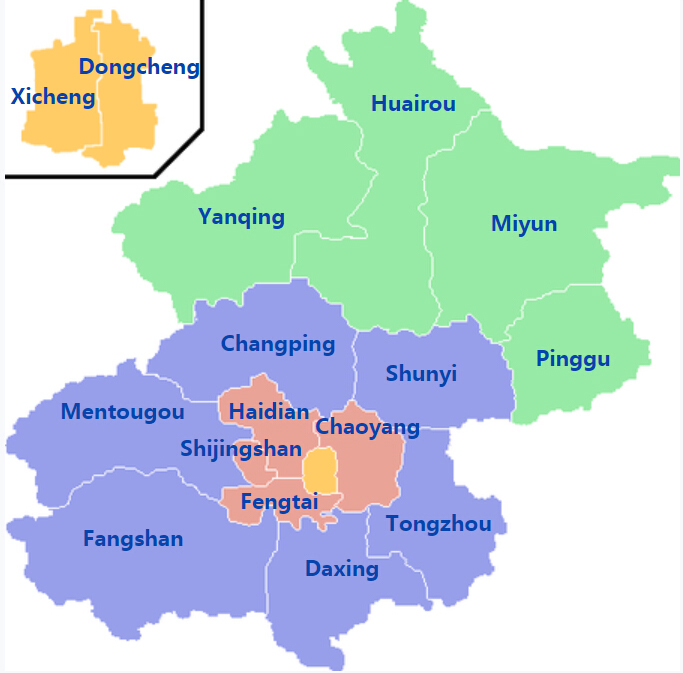
\includegraphics[width=0.5\linewidth]{beijing_map} \caption{Beijing District Map}\label{fig:pressure}
\end{figure}

\begin{enumerate}
\def\labelenumi{\arabic{enumi}.}
\setcounter{enumi}{14}
\tightlist
\item
  \textbf{\emph{district}}: (\emph{categorical}) There are 13 main
  districts in Beijing and each number from 1 to 13 refers to a
  different district in which the property lies in. In this case, 1
  refers to DongCheng, 2 refers to FengTai, 3 refers to YiZhuang, 4
  refers to DaXing, 5 refers to FangShan, 6 refers to ChangPing, 7
  refers to ChaoYang, 8 refers to HaiDian, 9 refers to ShiJingShan, 10
  refers to XiCheng, 11 refers to TongZhou, 12 refers to MenTouGou and
  13 refers to ShunYi.
\end{enumerate}

\hypertarget{response-variable}{%
\subsubsection{\texorpdfstring{\textbf{Response
Variable}}{Response Variable}}\label{response-variable}}

\begin{enumerate}
\def\labelenumi{\arabic{enumi}.}
\tightlist
\item
  \textbf{\emph{price}}: (\emph{integer}) The price per square foot of
  the property (price = totalPrice / square). To ensure that the price
  is a fair comparison across all the properties listed, we decided to
  compare the price per square foot of all properties instead of
  totalPrice. Since some properties may be bigger than others, comparing
  price per square foot provides us with a better understanding of how
  valuable a property is.
\end{enumerate}

Districts: 1-DongCheng 2-FengTai 3-YiZhuang 4-DaXing 5-FangShan
6-ChangPing 7-ChaoYang 8-HaiDian 9-ShiJingShan 10-XiCheng 11-TongZhou
12-MenTouGou 13-ShunYi

\hypertarget{section-2-data-cleaning}{%
\section{Section 2: Data Cleaning}\label{section-2-data-cleaning}}

\begin{Shaded}
\begin{Highlighting}[]
\CommentTok{\# loading libraries}
\FunctionTok{library}\NormalTok{(lubridate)}
\FunctionTok{library}\NormalTok{(dplyr)}
\FunctionTok{library}\NormalTok{(VIM)}
\FunctionTok{library}\NormalTok{(stringr)}
\FunctionTok{library}\NormalTok{(ggplot2)}
\FunctionTok{library}\NormalTok{(naniar)}
\end{Highlighting}
\end{Shaded}

\begin{Shaded}
\begin{Highlighting}[]
\CommentTok{\# the following code is used to import dataset that includes Chinese character}
\NormalTok{data }\OtherTok{\textless{}{-}} \FunctionTok{read.csv}\NormalTok{(}\StringTok{"new.csv"}\NormalTok{, }\AttributeTok{fileEncoding =} \StringTok{"GBK"}\NormalTok{, }\AttributeTok{encoding =} \StringTok{"GBK"}\NormalTok{)}
\end{Highlighting}
\end{Shaded}

\hypertarget{cleaning-trade-time-variable}{%
\subsection{2.1 Cleaning Trade Time
Variable}\label{cleaning-trade-time-variable}}

The \texttt{tradeTime} variable is in the format of y-m-d, we wanted to
look at year, month, and day separately. Therefore, we created new
variables \texttt{year}, \texttt{month}, \texttt{day} based on
\texttt{tradeTime}. \newline Since the current data has 318851 rows, we
decided to use part of the data where the trade time was in 2017.

\begin{Shaded}
\begin{Highlighting}[]
\NormalTok{data2017 }\OtherTok{\textless{}{-}}\NormalTok{ data }\SpecialCharTok{\%\textgreater{}\%} 
  \FunctionTok{mutate}\NormalTok{(}\AttributeTok{year =} \FunctionTok{year}\NormalTok{(tradeTime), }\AttributeTok{month =}\NormalTok{ month.name[}\FunctionTok{month}\NormalTok{(tradeTime)], }\AttributeTok{day =} \FunctionTok{day}\NormalTok{(tradeTime)) }\SpecialCharTok{\%\textgreater{}\%}
  \FunctionTok{filter}\NormalTok{(year }\SpecialCharTok{==} \DecValTok{2017}\NormalTok{)}
\end{Highlighting}
\end{Shaded}

\hypertarget{cleaning-floor-variable}{%
\subsection{2.2 Cleaning Floor Variable}\label{cleaning-floor-variable}}

The \texttt{floor} variable two piece of information. The first part,
which is in Chinese character, informs the floor range of the
apartment/house. The second part, which is a number, tells us the total
number of floors the building has. Therefore, we need to separate these
two information into two new variables (\texttt{totalFloor} and
\texttt{floorRange}) to better analyze them. At the same time, we
converted Chinese characters into English.

\hypertarget{cleaning-variable-format}{%
\subsection{2.3 Cleaning variable
format}\label{cleaning-variable-format}}

Some variables such as living room and bedroom should be numerical
variable, while other variables such as subway and elevator should be
categorical variables. We also recoded the district variable into
district names, which will be easier to see for later analysis. Finally,
the living room in this dataset should be bedroom and drawing room in
this dataset should be living room.

\begin{Shaded}
\begin{Highlighting}[]
\NormalTok{data2017 }\OtherTok{\textless{}{-}}\NormalTok{ data2017 }\SpecialCharTok{\%\textgreater{}\%} 
  \FunctionTok{rename}\NormalTok{(}\AttributeTok{livingRoom =}\NormalTok{ drawingRoom, }\AttributeTok{bedRoom =}\NormalTok{ livingRoom) }\SpecialCharTok{\%\textgreater{}\%}
  \FunctionTok{mutate}\NormalTok{(}\AttributeTok{constructionTime =} \FunctionTok{as.numeric}\NormalTok{(constructionTime), }
         \AttributeTok{livingRoom =} \FunctionTok{as.numeric}\NormalTok{(livingRoom),}
         \AttributeTok{bedRoom =} \FunctionTok{as.numeric}\NormalTok{(bedRoom),}
         \AttributeTok{bathRoom =} \FunctionTok{as.numeric}\NormalTok{(bathRoom),}
         \AttributeTok{kitchen =} \FunctionTok{as.numeric}\NormalTok{(kitchen),}
         \AttributeTok{subway =} \FunctionTok{as.factor}\NormalTok{(subway),}
         \AttributeTok{elevator =} \FunctionTok{as.factor}\NormalTok{(elevator),}
         \AttributeTok{fiveYearsProperty =} \FunctionTok{as.factor}\NormalTok{(fiveYearsProperty),}
         \AttributeTok{district =} \FunctionTok{recode}\NormalTok{(district, }\StringTok{"1"} \OtherTok{=} \StringTok{"DongCheng"}\NormalTok{,}
                           \StringTok{"2"} \OtherTok{=} \StringTok{"FengTai"}\NormalTok{, }\StringTok{"3"} \OtherTok{=} \StringTok{"YiZhuang"}\NormalTok{, }\StringTok{"4"} \OtherTok{=} \StringTok{"DaXing"}\NormalTok{, }
                           \StringTok{"5"} \OtherTok{=} \StringTok{"FangShan"}\NormalTok{, }\StringTok{"6"} \OtherTok{=} \StringTok{"ChangPing"}\NormalTok{, }\StringTok{"7"} \OtherTok{=} \StringTok{"ChaoYang"}\NormalTok{,}
                           \StringTok{"8"} \OtherTok{=} \StringTok{"HaiDian"}\NormalTok{, }\StringTok{"9"} \OtherTok{=} \StringTok{"ShiJingShan"}\NormalTok{, }\StringTok{"10"} \OtherTok{=} \StringTok{"XiCheng"}\NormalTok{, }
                           \StringTok{"11"} \OtherTok{=} \StringTok{"TongZhou"}\NormalTok{, }\StringTok{"12"} \OtherTok{=} \StringTok{"MenTouGou"}\NormalTok{, }\StringTok{"13"} \OtherTok{=} \StringTok{"ShunYi"}\NormalTok{))}
\end{Highlighting}
\end{Shaded}

\hypertarget{missing-values}{%
\subsection{2.4 Missing Values}\label{missing-values}}

\begin{Shaded}
\begin{Highlighting}[]
\FunctionTok{table}\NormalTok{(}\FunctionTok{is.na}\NormalTok{(data2017))}
\end{Highlighting}
\end{Shaded}

\begin{verbatim}
## 
##   FALSE    TRUE 
## 1338424    1303
\end{verbatim}

\begin{Shaded}
\begin{Highlighting}[]
\NormalTok{na\_plot }\OtherTok{\textless{}{-}} \FunctionTok{aggr}\NormalTok{(data2017, }\AttributeTok{col=}\FunctionTok{c}\NormalTok{(}\StringTok{\textquotesingle{}skyblue\textquotesingle{}}\NormalTok{,}\StringTok{\textquotesingle{}red\textquotesingle{}}\NormalTok{), }\AttributeTok{numbers=}\ConstantTok{TRUE}\NormalTok{, }\AttributeTok{sortVars=}\ConstantTok{TRUE}\NormalTok{, }
                \AttributeTok{labels=}\FunctionTok{names}\NormalTok{(data2017), }\AttributeTok{cex.axis=}\NormalTok{.}\DecValTok{4}\NormalTok{, }\AttributeTok{gap=}\DecValTok{3}\NormalTok{, }\AttributeTok{ylab=}\FunctionTok{c}\NormalTok{(}\StringTok{"Missing data"}\NormalTok{,}\StringTok{"Pattern"}\NormalTok{))}
\end{Highlighting}
\end{Shaded}

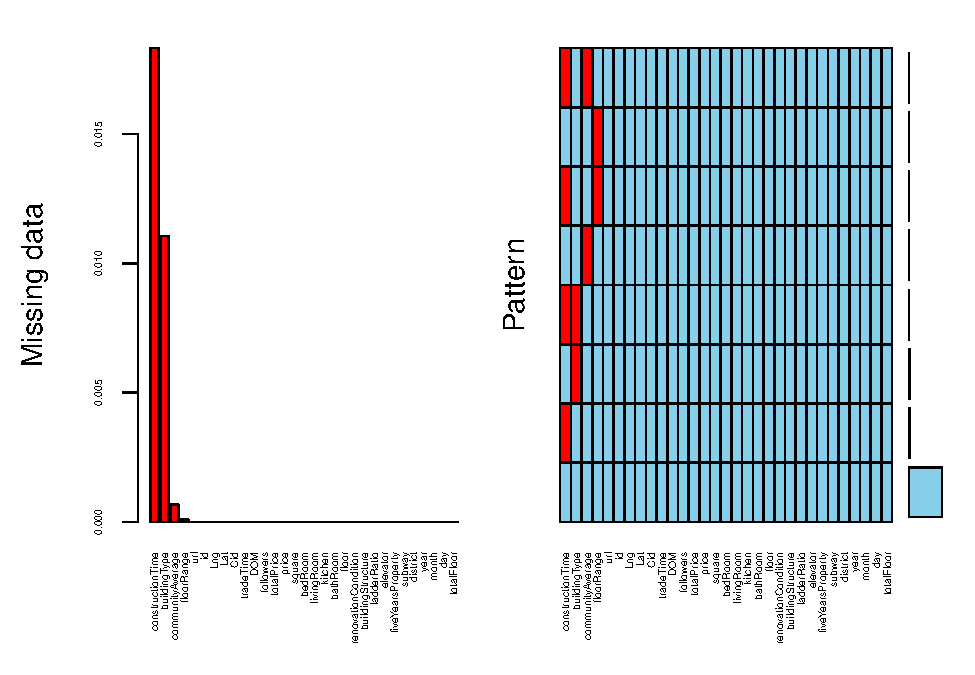
\includegraphics{Project_files/figure-latex/unnamed-chunk-6-1.pdf}

\begin{verbatim}
## 
##  Variables sorted by number of missings: 
##             Variable        Count
##     constructionTime 1.832612e-02
##         buildingType 1.106046e-02
##     communityAverage 6.710322e-04
##           floorRange 9.255617e-05
##                  url 0.000000e+00
##                   id 0.000000e+00
##                  Lng 0.000000e+00
##                  Lat 0.000000e+00
##                  Cid 0.000000e+00
##            tradeTime 0.000000e+00
##                  DOM 0.000000e+00
##            followers 0.000000e+00
##           totalPrice 0.000000e+00
##                price 0.000000e+00
##               square 0.000000e+00
##              bedRoom 0.000000e+00
##           livingRoom 0.000000e+00
##              kitchen 0.000000e+00
##             bathRoom 0.000000e+00
##                floor 0.000000e+00
##  renovationCondition 0.000000e+00
##    buildingStructure 0.000000e+00
##          ladderRatio 0.000000e+00
##             elevator 0.000000e+00
##    fiveYearsProperty 0.000000e+00
##               subway 0.000000e+00
##             district 0.000000e+00
##                 year 0.000000e+00
##                month 0.000000e+00
##                  day 0.000000e+00
##           totalFloor 0.000000e+00
\end{verbatim}

Our data had 1303 missing values. All missing values are in variables
construction time, building type, community average, and floor range.
The above graph shows the proportion of missing values in each variable
with the highest being 0.018 for construction time. \newline We decided
to remove all missing values for two reasons. First, 1303 missing values
is a relatively small amount of data compared to 43217 observations we
have. Second, we did not plan to use the variable buildingType and
community average, which had a large portion of missing values.

\begin{Shaded}
\begin{Highlighting}[]
\NormalTok{data2017 }\OtherTok{\textless{}{-}} \FunctionTok{na.omit}\NormalTok{(data2017)}
\end{Highlighting}
\end{Shaded}

Now we have 42710 observations.

\hypertarget{remove-unnecessary-variables}{%
\subsection{2.5 Remove unnecessary
variables}\label{remove-unnecessary-variables}}

The final step of data cleaning is removing variables that we do not
plan to use.

\begin{Shaded}
\begin{Highlighting}[]
\NormalTok{data2017 }\OtherTok{\textless{}{-}}\NormalTok{ data2017 }\SpecialCharTok{\%\textgreater{}\%}
  \FunctionTok{select}\NormalTok{(}\SpecialCharTok{{-}}\FunctionTok{c}\NormalTok{(url, Lng, Lat, Cid, tradeTime, floor, buildingType, communityAverage, year))}
\end{Highlighting}
\end{Shaded}

\hypertarget{section-3-exploratory-analysis}{%
\section{Section 3: Exploratory
Analysis}\label{section-3-exploratory-analysis}}

\hypertarget{distribution-of-variables-and-outliers}{%
\subsection{3.1 Distribution of variables and
outliers}\label{distribution-of-variables-and-outliers}}

\hypertarget{month}{%
\subsubsection{3.1.1 Month}\label{month}}

\begin{Shaded}
\begin{Highlighting}[]
\FunctionTok{ggplot}\NormalTok{(data2017, }\FunctionTok{aes}\NormalTok{(}\AttributeTok{x =}\NormalTok{ month)) }\SpecialCharTok{+} 
  \FunctionTok{geom\_bar}\NormalTok{(}\AttributeTok{fill =} \StringTok{"light blue"}\NormalTok{) }\SpecialCharTok{+} 
  \FunctionTok{scale\_x\_discrete}\NormalTok{(}\AttributeTok{limits =}\NormalTok{ month.name)}
\end{Highlighting}
\end{Shaded}

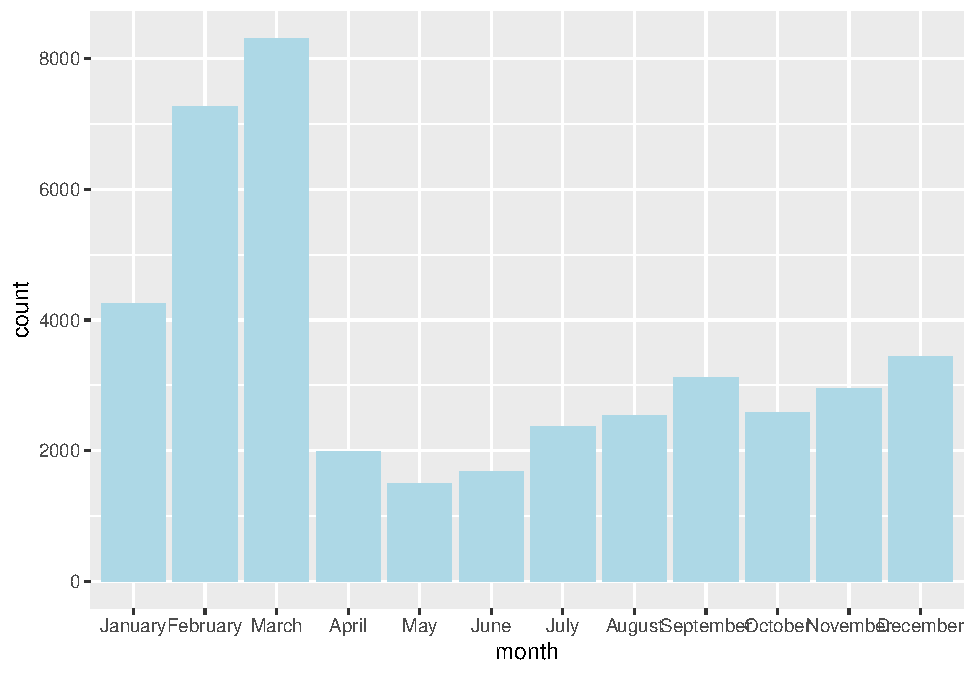
\includegraphics{Project_files/figure-latex/unnamed-chunk-9-1.pdf}

The first three months of year 2017 had the most trading of houses, with
March being the highest number of trading, more than 8000 tradings.
Apirl, May, and June each only had less than 1/4 of the number of
trading compared to March. The amount of transactions for the rest of
the year remained below 4000.

\hypertarget{day}{%
\subsubsection{3.1.2 Day}\label{day}}

\begin{Shaded}
\begin{Highlighting}[]
\FunctionTok{ggplot}\NormalTok{(data2017, }\FunctionTok{aes}\NormalTok{(}\AttributeTok{x =}\NormalTok{ day)) }\SpecialCharTok{+} 
  \FunctionTok{geom\_bar}\NormalTok{(}\AttributeTok{fill =} \StringTok{"light blue"}\NormalTok{, }\AttributeTok{color =} \StringTok{"black"}\NormalTok{)}
\end{Highlighting}
\end{Shaded}

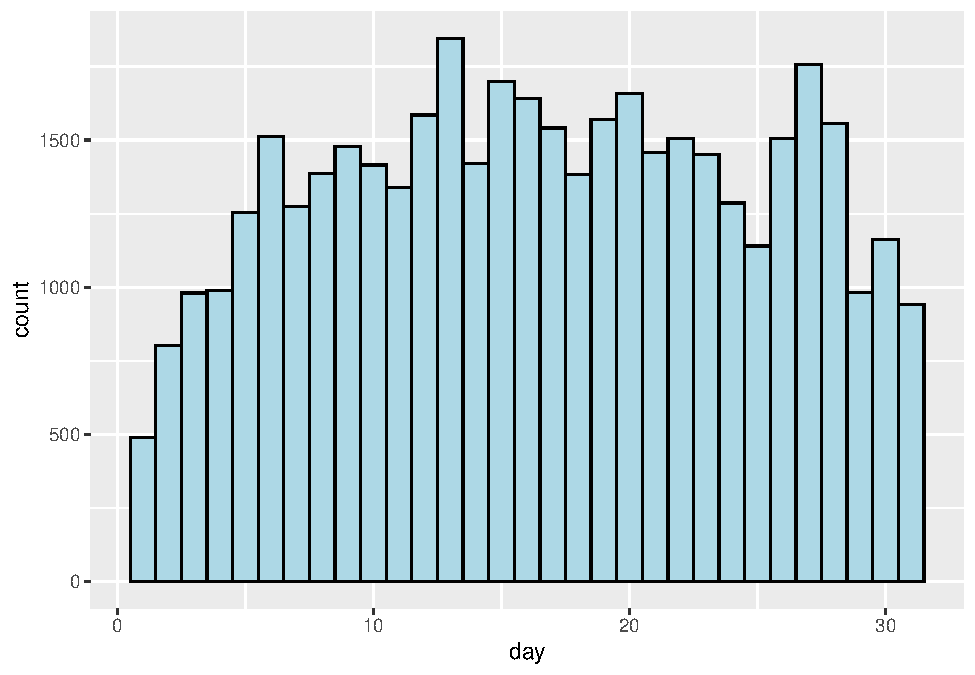
\includegraphics{Project_files/figure-latex/unnamed-chunk-10-1.pdf}
There isn't a unique day of the month that people liked to buy houses,
but people relatively like to buy houses in the middle of the month. Few
trades happened in the beginning of the month.

\hypertarget{total-floor}{%
\subsubsection{3.1.3 Total Floor}\label{total-floor}}

\begin{Shaded}
\begin{Highlighting}[]
\FunctionTok{ggplot}\NormalTok{(data2017, }\FunctionTok{aes}\NormalTok{(}\AttributeTok{x =}\NormalTok{ totalFloor)) }\SpecialCharTok{+} \FunctionTok{geom\_histogram}\NormalTok{(}\AttributeTok{color =} \StringTok{"black"}\NormalTok{, }\AttributeTok{fill =} \StringTok{"blue"}\NormalTok{) }
\end{Highlighting}
\end{Shaded}

\begin{verbatim}
## `stat_bin()` using `bins = 30`. Pick better value with `binwidth`.
\end{verbatim}

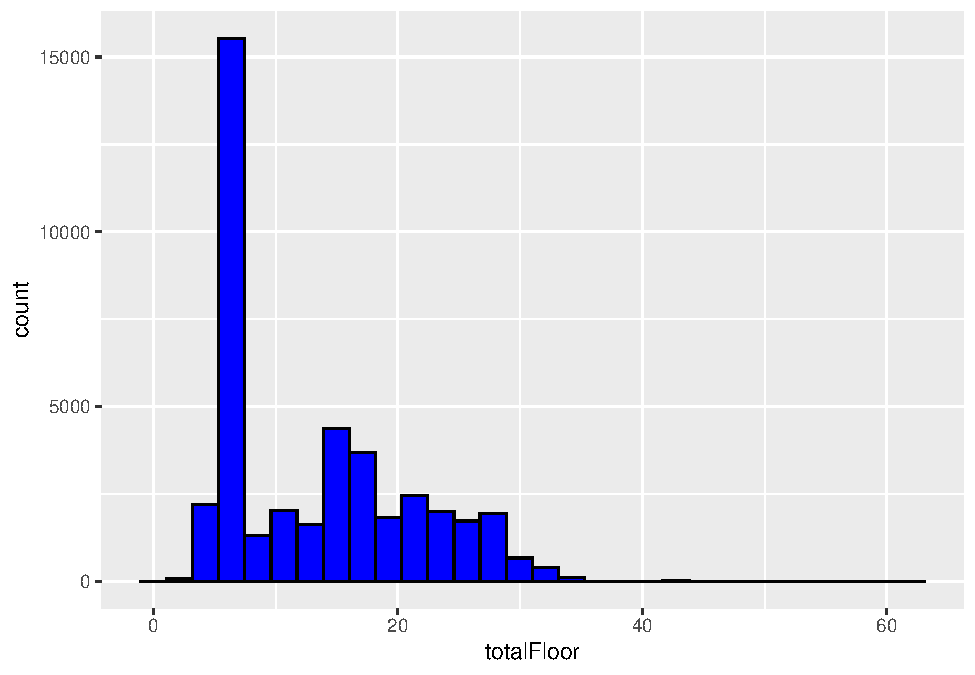
\includegraphics{Project_files/figure-latex/unnamed-chunk-11-1.pdf}

\begin{Shaded}
\begin{Highlighting}[]
\FunctionTok{summary}\NormalTok{(data2017}\SpecialCharTok{$}\NormalTok{totalFloor)}
\end{Highlighting}
\end{Shaded}

\begin{verbatim}
##    Min. 1st Qu.  Median    Mean 3rd Qu.    Max. 
##    1.00    6.00   11.00   13.38   20.00   63.00
\end{verbatim}

\begin{Shaded}
\begin{Highlighting}[]
\NormalTok{data2017 }\SpecialCharTok{\%\textgreater{}\%} \FunctionTok{arrange}\NormalTok{(}\FunctionTok{desc}\NormalTok{(totalFloor)) }\SpecialCharTok{\%\textgreater{}\%} \FunctionTok{select}\NormalTok{(id, totalFloor, floorRange) }\SpecialCharTok{\%\textgreater{}\%} \FunctionTok{head}\NormalTok{()}
\end{Highlighting}
\end{Shaded}

\begin{verbatim}
##             id totalFloor floorRange
## 1 101101127418         63        low
## 2 101101690389         57     midium
## 3 101091696453         42        low
## 4 101100641538         42        low
## 5 101100768834         42       high
## 6 101100791635         42     midium
\end{verbatim}

\begin{Shaded}
\begin{Highlighting}[]
\NormalTok{data2017 }\OtherTok{\textless{}{-}}\NormalTok{ data2017 }\SpecialCharTok{\%\textgreater{}\%}
  \FunctionTok{filter}\NormalTok{(totalFloor }\SpecialCharTok{\textless{}} \DecValTok{60}\NormalTok{)}
\end{Highlighting}
\end{Shaded}

The distribution of total floor is unimodel and skewed to the right.
There are quite a few very tall buildings, but such high numbers could
be an error in data recording. The url for the apartment located in a
building with 63 floors is invalid; however, we checked the apartment
located in the building with 57 floors using url and, surprisingly, the
building does exist and is called Yu Jin Tai. Therefore, we only removed
the trade with total floor of 63.

\hypertarget{floor-range}{%
\subsubsection{3.1.4 Floor Range}\label{floor-range}}

\begin{Shaded}
\begin{Highlighting}[]
\FunctionTok{ggplot}\NormalTok{(data2017, }\FunctionTok{aes}\NormalTok{(}\AttributeTok{x =}\NormalTok{ floorRange)) }\SpecialCharTok{+} 
  \FunctionTok{geom\_bar}\NormalTok{(}\AttributeTok{fill =} \StringTok{"light blue"}\NormalTok{) }\SpecialCharTok{+}
  \FunctionTok{scale\_x\_discrete}\NormalTok{(}\AttributeTok{limits =} \FunctionTok{c}\NormalTok{(}\StringTok{"bottom"}\NormalTok{, }\StringTok{"low"}\NormalTok{, }\StringTok{"midium"}\NormalTok{, }\StringTok{"high"}\NormalTok{, }\StringTok{"top"}\NormalTok{)) }
\end{Highlighting}
\end{Shaded}

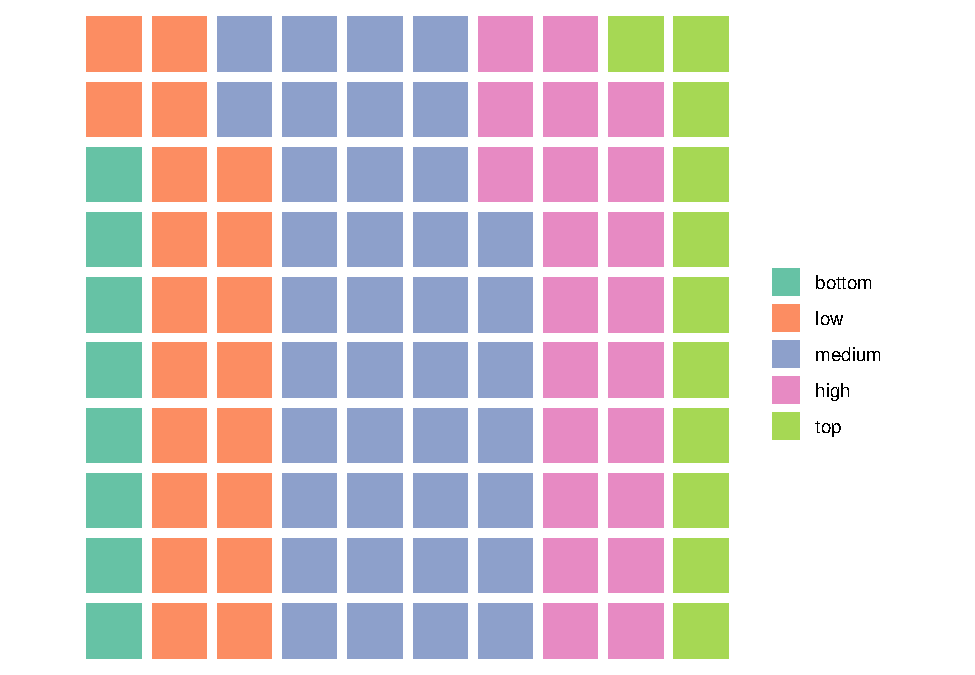
\includegraphics{Project_files/figure-latex/unnamed-chunk-12-1.pdf}
Apartments located in the middle of a building were traded the most in
2017.

\hypertarget{dom}{%
\subsubsection{3.1.5 DOM}\label{dom}}

The graph of number of days on market is unimodal and heavily skewed to
the right. The mean number of days on market is around 51 and the median
is 31 days. Approximately 2.5\% of values are below 2. Approximately
2.5\% of values are above 196. The longest day on market is 721. Whereas
there are total of 474 houses have less or equal to 1 day on market
until sold.

\begin{Shaded}
\begin{Highlighting}[]
\FunctionTok{ggplot}\NormalTok{(data2017, }\FunctionTok{aes}\NormalTok{(}\AttributeTok{x=}\NormalTok{DOM))}\SpecialCharTok{+}
  \FunctionTok{geom\_histogram}\NormalTok{(}\AttributeTok{fill=}\StringTok{\textquotesingle{}lightblue\textquotesingle{}}\NormalTok{, }\AttributeTok{color=}\StringTok{\textquotesingle{}black\textquotesingle{}}\NormalTok{) }\SpecialCharTok{+}
  \FunctionTok{xlab}\NormalTok{(}\StringTok{"DOM"}\NormalTok{)}\SpecialCharTok{+}\FunctionTok{ylab}\NormalTok{(}\StringTok{"Count"}\NormalTok{)}\SpecialCharTok{+}\FunctionTok{ggtitle}\NormalTok{(}\StringTok{"Active Days on Market Histogram"}\NormalTok{)}
\end{Highlighting}
\end{Shaded}

\begin{verbatim}
## `stat_bin()` using `bins = 30`. Pick better value with `binwidth`.
\end{verbatim}

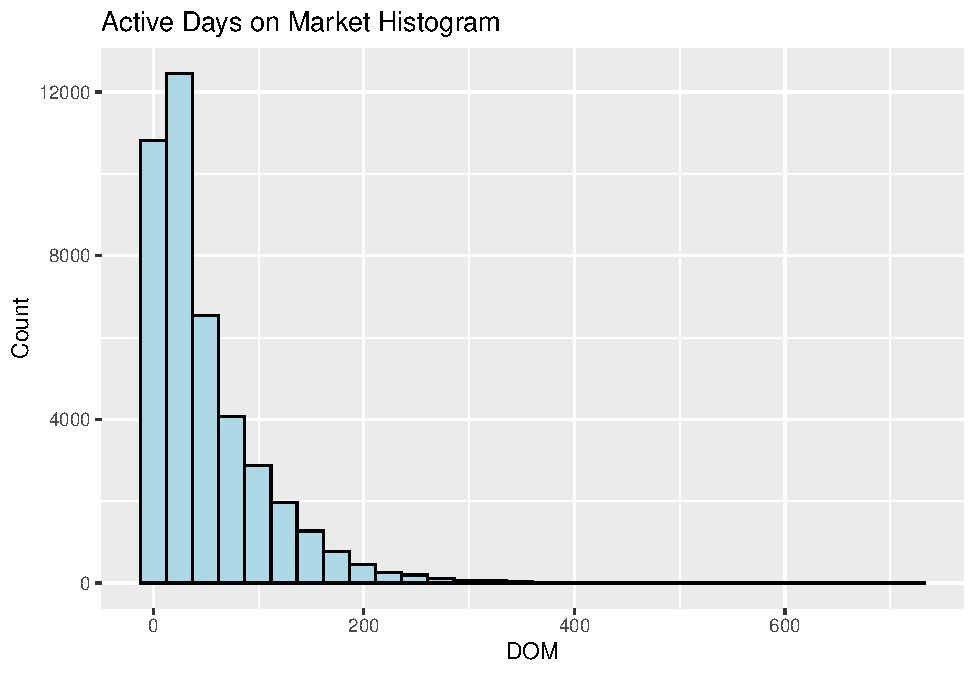
\includegraphics{Project_files/figure-latex/unnamed-chunk-13-1.pdf}

\begin{Shaded}
\begin{Highlighting}[]
\FunctionTok{mean}\NormalTok{(data2017}\SpecialCharTok{$}\NormalTok{DOM)}
\end{Highlighting}
\end{Shaded}

\begin{verbatim}
## [1] 50.858
\end{verbatim}

\begin{Shaded}
\begin{Highlighting}[]
\FunctionTok{quantile}\NormalTok{(data2017}\SpecialCharTok{$}\NormalTok{DOM, }\FunctionTok{c}\NormalTok{(}\DecValTok{0}\NormalTok{, }\FloatTok{0.025}\NormalTok{, }\FloatTok{0.25}\NormalTok{, }\FloatTok{0.5}\NormalTok{, }\FloatTok{0.75}\NormalTok{, }\FloatTok{0.975}\NormalTok{, }\DecValTok{1}\NormalTok{))}
\end{Highlighting}
\end{Shaded}

\begin{verbatim}
##    0%  2.5%   25%   50%   75% 97.5%  100% 
##     1     2    12    31    71   196   721
\end{verbatim}

\begin{Shaded}
\begin{Highlighting}[]
\NormalTok{data2017 }\SpecialCharTok{\%\textgreater{}\%}
  \FunctionTok{filter}\NormalTok{(DOM}\SpecialCharTok{\textless{}=}\DecValTok{1}\NormalTok{) }\SpecialCharTok{\%\textgreater{}\%}
  \FunctionTok{nrow}\NormalTok{()  }\CommentTok{\# number of houses have less than 1 day on market}
\end{Highlighting}
\end{Shaded}

\begin{verbatim}
## [1] 474
\end{verbatim}

\hypertarget{followers}{%
\subsubsection{3.1.6 followers}\label{followers}}

The graph of number of followers is unimodal and heavily skewed to the
right. The mean is around 49 people and the median is around 31 people.
Approximately 2.5\% of values are below or equal to 0. Approximately
2.5\% of values are above 216. However, the highest 2.5\% are jumps from
216 to 1143, which suggests that there are a few significantly popular
houses. There are 5617 houses with 0 follower and also a total of 5
houses with more than 1000 followers. Among these houses with more than
1000 followers, 1 house has significant low total price compare with
other houses. However, it also has relative small area and is located in
the suburb, which makes this reasonable.

\begin{Shaded}
\begin{Highlighting}[]
\FunctionTok{ggplot}\NormalTok{(data2017, }\FunctionTok{aes}\NormalTok{(}\AttributeTok{x=}\NormalTok{followers))}\SpecialCharTok{+}
  \FunctionTok{geom\_histogram}\NormalTok{(}\AttributeTok{fill=}\StringTok{\textquotesingle{}lightblue\textquotesingle{}}\NormalTok{, }\AttributeTok{color=}\StringTok{\textquotesingle{}black\textquotesingle{}}\NormalTok{) }\SpecialCharTok{+}
  \FunctionTok{xlab}\NormalTok{(}\StringTok{"followers"}\NormalTok{)}\SpecialCharTok{+}\FunctionTok{ylab}\NormalTok{(}\StringTok{"Count"}\NormalTok{)}\SpecialCharTok{+}
  \FunctionTok{ggtitle}\NormalTok{(}\StringTok{"followers Histogram"}\NormalTok{)}
\end{Highlighting}
\end{Shaded}

\begin{verbatim}
## `stat_bin()` using `bins = 30`. Pick better value with `binwidth`.
\end{verbatim}

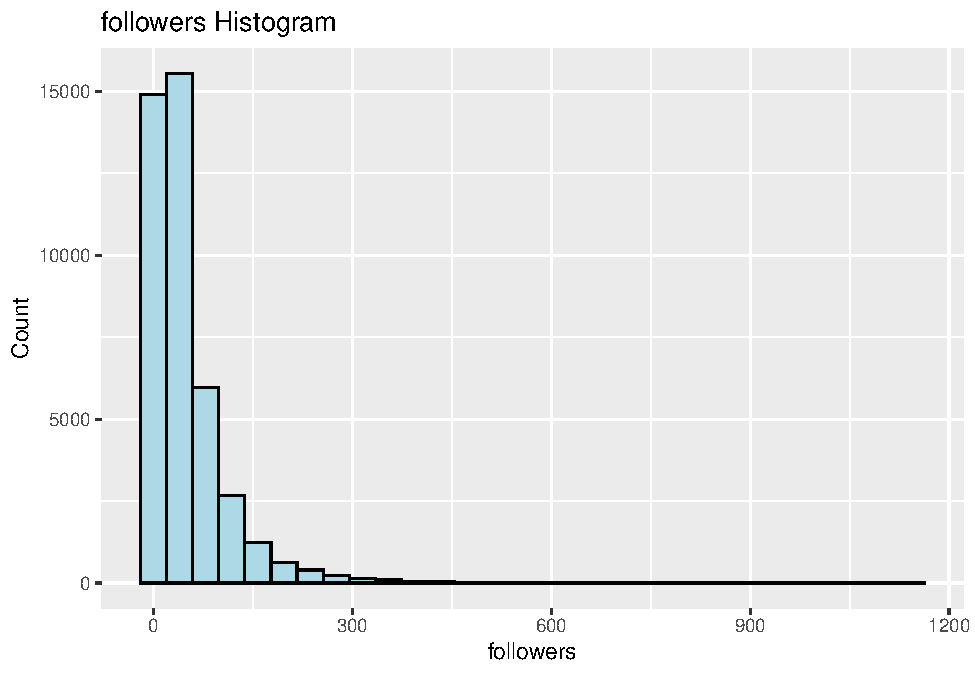
\includegraphics{Project_files/figure-latex/unnamed-chunk-14-1.pdf}

\begin{Shaded}
\begin{Highlighting}[]
\FunctionTok{mean}\NormalTok{(data2017}\SpecialCharTok{$}\NormalTok{followers)}
\end{Highlighting}
\end{Shaded}

\begin{verbatim}
## [1] 49.41241
\end{verbatim}

\begin{Shaded}
\begin{Highlighting}[]
\FunctionTok{quantile}\NormalTok{(data2017}\SpecialCharTok{$}\NormalTok{followers, }\FunctionTok{c}\NormalTok{(}\DecValTok{0}\NormalTok{, }\FloatTok{0.025}\NormalTok{, }\FloatTok{0.25}\NormalTok{, }\FloatTok{0.5}\NormalTok{, }\FloatTok{0.75}\NormalTok{, }\FloatTok{0.975}\NormalTok{, }\DecValTok{1}\NormalTok{))}
\end{Highlighting}
\end{Shaded}

\begin{verbatim}
##    0%  2.5%   25%   50%   75% 97.5%  100% 
##     0     0    11    31    64   216  1143
\end{verbatim}

\begin{Shaded}
\begin{Highlighting}[]
\NormalTok{data2017 }\SpecialCharTok{\%\textgreater{}\%} \FunctionTok{filter}\NormalTok{(followers}\SpecialCharTok{\textgreater{}}\DecValTok{1000}\NormalTok{)}
\end{Highlighting}
\end{Shaded}

\begin{verbatim}
##             id DOM followers totalPrice  price square bedRoom livingRoom
## 1 101100732988 132      1085       48.0  26667  18.00       1          1
## 2 101100746033 141      1015      297.5  78393  37.95       1          0
## 3 101101590746 229      1143      380.0 116780  32.54       1          1
## 4 101102303199  25      1045      514.0  87415  58.80       2          1
##   kitchen bathRoom constructionTime renovationCondition buildingStructure
## 1       1        1             2011                   4                 6
## 2       1        1             2007                   4                 6
## 3       1        2             2005                   3                 6
## 4       1        1             1992                   4                 2
##   ladderRatio elevator fiveYearsProperty subway  district    month day
## 1       0.385        1                 0      0 ChangPing February  24
## 2       0.250        1                 1      1  ChaoYang    March   9
## 3       0.077        1                 1      1   XiCheng December  31
## 4       0.500        0                 1      1   HaiDian December   8
##   totalFloor floorRange
## 1         28     midium
## 2         12       high
## 3         10     midium
## 4          6       high
\end{verbatim}

\hypertarget{totalprice}{%
\subsubsection{3.1.7 totalPrice}\label{totalprice}}

The graph of total price is diamond-shaped, unimodal, and skews right.
The average total price of a house in Beijing in 2017 is 526x10,000 yuan
(around 750\textasciitilde810 thousands dollars depend on inflation) and
the median is 460x10,000 yuan (around 660\textasciitilde710 thousands
dollars). Approximately 2.5\% of values are below 215x10,000 yuan.
Approximately 2.5\% of values are above 1250x10,000 yuan.

\begin{Shaded}
\begin{Highlighting}[]
\FunctionTok{ggplot}\NormalTok{(data2017, }\FunctionTok{aes}\NormalTok{(}\AttributeTok{x=}\NormalTok{totalPrice))}\SpecialCharTok{+}
  \FunctionTok{geom\_histogram}\NormalTok{(}\AttributeTok{fill=}\StringTok{\textquotesingle{}lightblue\textquotesingle{}}\NormalTok{, }\AttributeTok{color=}\StringTok{\textquotesingle{}black\textquotesingle{}}\NormalTok{) }\SpecialCharTok{+}
  \FunctionTok{xlab}\NormalTok{(}\StringTok{"totalPrice"}\NormalTok{)}\SpecialCharTok{+}\FunctionTok{ylab}\NormalTok{(}\StringTok{"Count"}\NormalTok{)}\SpecialCharTok{+}\FunctionTok{ggtitle}\NormalTok{(}\StringTok{"Total price (in 10,000yuan) Histogram"}\NormalTok{)}
\end{Highlighting}
\end{Shaded}

\begin{verbatim}
## `stat_bin()` using `bins = 30`. Pick better value with `binwidth`.
\end{verbatim}

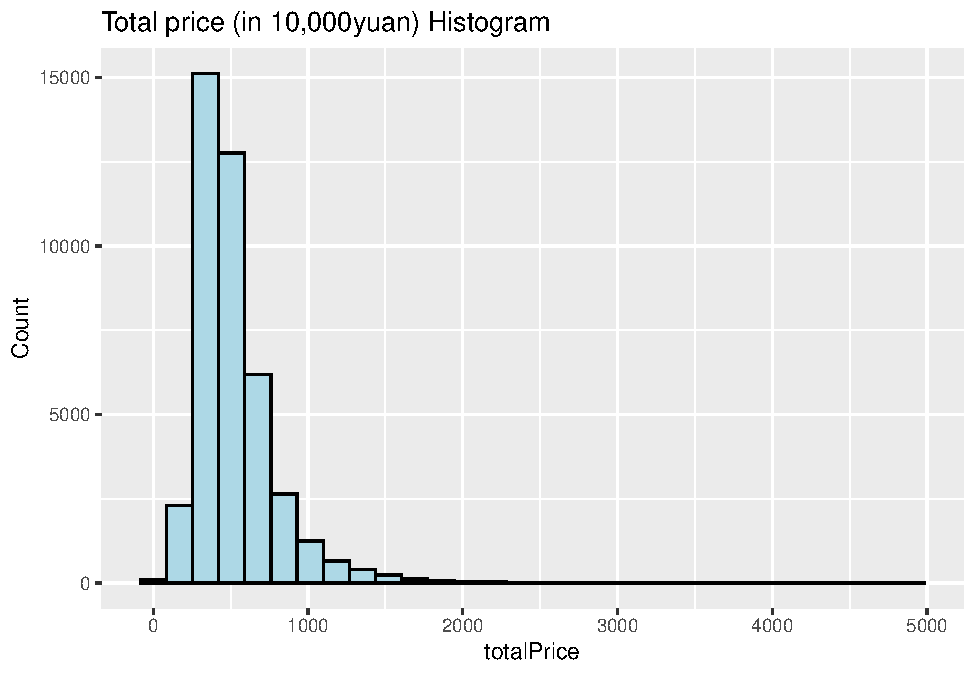
\includegraphics{Project_files/figure-latex/unnamed-chunk-15-1.pdf}

\begin{Shaded}
\begin{Highlighting}[]
\FunctionTok{mean}\NormalTok{(data2017}\SpecialCharTok{$}\NormalTok{totalPrice)}
\end{Highlighting}
\end{Shaded}

\begin{verbatim}
## [1] 526.3465
\end{verbatim}

\begin{Shaded}
\begin{Highlighting}[]
\FunctionTok{quantile}\NormalTok{(data2017}\SpecialCharTok{$}\NormalTok{totalPrice, }\FunctionTok{c}\NormalTok{(}\DecValTok{0}\NormalTok{, }\FloatTok{0.025}\NormalTok{, }\FloatTok{0.25}\NormalTok{, }\FloatTok{0.5}\NormalTok{, }\FloatTok{0.75}\NormalTok{, }\FloatTok{0.975}\NormalTok{, }\DecValTok{1}\NormalTok{))}
\end{Highlighting}
\end{Shaded}

\begin{verbatim}
##     0%   2.5%    25%    50%    75%  97.5%   100% 
##    1.0  215.5  355.0  460.0  616.0 1250.0 4900.0
\end{verbatim}

\begin{Shaded}
\begin{Highlighting}[]
\FunctionTok{ggplot}\NormalTok{(data2017, }\FunctionTok{aes}\NormalTok{(}\AttributeTok{x=}\NormalTok{district,}\AttributeTok{y=}\NormalTok{totalPrice))}\SpecialCharTok{+}
  \FunctionTok{geom\_boxplot}\NormalTok{()}\SpecialCharTok{+}
  \FunctionTok{theme}\NormalTok{(}\AttributeTok{axis.text.x =} \FunctionTok{element\_text}\NormalTok{(}\AttributeTok{angle =} \DecValTok{45}\NormalTok{, }\AttributeTok{vjust =} \FloatTok{0.5}\NormalTok{, }\AttributeTok{hjust=}\DecValTok{1}\NormalTok{))}
\end{Highlighting}
\end{Shaded}

\includegraphics{Project_files/figure-latex/unnamed-chunk-15-2.pdf}

\hypertarget{price}{%
\subsubsection{3.1.8 price}\label{price}}

The graph for price is Diamond-shaped, unimodal, and skewed right. The
average price per square meter is around 67,430 yuan and median is
62,670 yuan, which are close. Approximately 2.5\% of values are above
127,359 yuan. Approximately 2.5\% of values are below 33,035 yuan. The
house that has the lowest value has 136 yuan per square meter, which is
about 20 dollars per square meter. Such low price doesn't make sense in
any part of Beijing. Therefore, we decided to remove this outlier.

\begin{Shaded}
\begin{Highlighting}[]
\FunctionTok{ggplot}\NormalTok{(data2017, }\FunctionTok{aes}\NormalTok{(}\AttributeTok{x=}\NormalTok{price))}\SpecialCharTok{+}
  \FunctionTok{geom\_histogram}\NormalTok{(}\AttributeTok{fill=}\StringTok{\textquotesingle{}lightblue\textquotesingle{}}\NormalTok{, }\AttributeTok{color=}\StringTok{\textquotesingle{}black\textquotesingle{}}\NormalTok{) }\SpecialCharTok{+}
  \FunctionTok{xlab}\NormalTok{(}\StringTok{"price"}\NormalTok{)}\SpecialCharTok{+}\FunctionTok{ylab}\NormalTok{(}\StringTok{"Count"}\NormalTok{)}\SpecialCharTok{+}\FunctionTok{ggtitle}\NormalTok{(}\StringTok{"Average price per square meter (in yuan) Histogram"}\NormalTok{)}
\end{Highlighting}
\end{Shaded}

\begin{verbatim}
## `stat_bin()` using `bins = 30`. Pick better value with `binwidth`.
\end{verbatim}

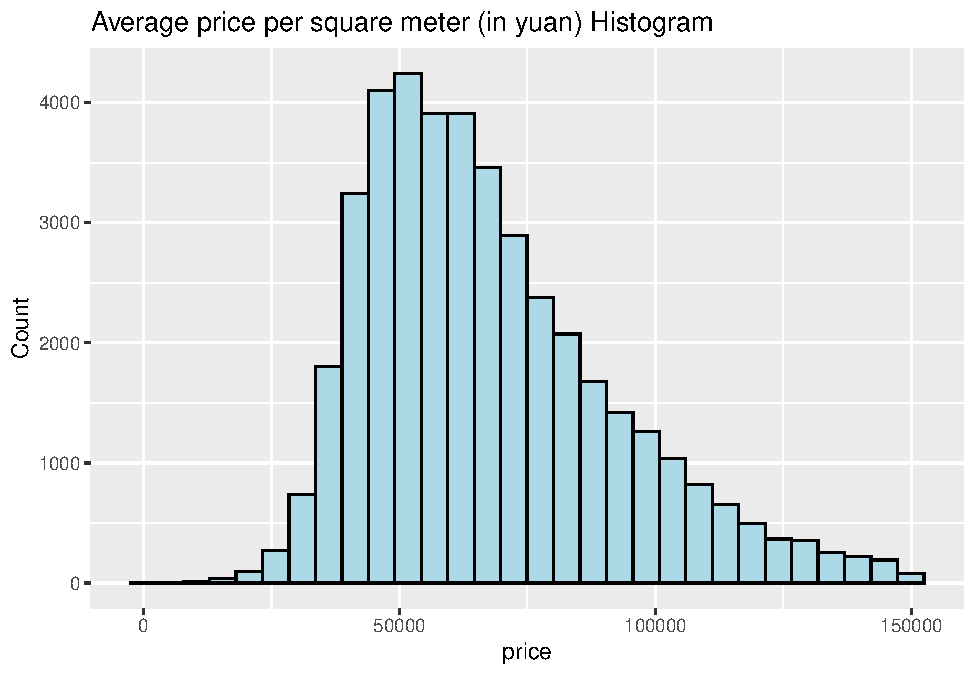
\includegraphics{Project_files/figure-latex/unnamed-chunk-16-1.pdf}

\begin{Shaded}
\begin{Highlighting}[]
\FunctionTok{mean}\NormalTok{(data2017}\SpecialCharTok{$}\NormalTok{price)}
\end{Highlighting}
\end{Shaded}

\begin{verbatim}
## [1] 67428.99
\end{verbatim}

\begin{Shaded}
\begin{Highlighting}[]
\FunctionTok{quantile}\NormalTok{(data2017}\SpecialCharTok{$}\NormalTok{price, }\FunctionTok{c}\NormalTok{(}\DecValTok{0}\NormalTok{, }\FloatTok{0.025}\NormalTok{, }\FloatTok{0.25}\NormalTok{, }\FloatTok{0.5}\NormalTok{, }\FloatTok{0.75}\NormalTok{, }\FloatTok{0.975}\NormalTok{, }\DecValTok{1}\NormalTok{))}
\end{Highlighting}
\end{Shaded}

\begin{verbatim}
##        0%      2.5%       25%       50%       75%     97.5%      100% 
##    136.00  33034.15  49330.00  62669.00  81075.50 127358.70 150000.00
\end{verbatim}

\begin{Shaded}
\begin{Highlighting}[]
\NormalTok{data2017 }\SpecialCharTok{\%\textgreater{}\%}
  \FunctionTok{filter}\NormalTok{(price}\SpecialCharTok{\textless{}=}\DecValTok{1000}\NormalTok{) }
\end{Highlighting}
\end{Shaded}

\begin{verbatim}
##             id DOM followers totalPrice price square bedRoom livingRoom kitchen
## 1 101101646066   2         0          1   136   73.8       2          1       1
##   bathRoom constructionTime renovationCondition buildingStructure ladderRatio
## 1        1             1993                   1                 6         0.2
##   elevator fiveYearsProperty subway district month day totalFloor floorRange
## 1        1                 0      0  HaiDian  June   2         18     bottom
\end{verbatim}

\begin{Shaded}
\begin{Highlighting}[]
\NormalTok{data2017 }\OtherTok{\textless{}{-}}\NormalTok{ data2017 }\SpecialCharTok{\%\textgreater{}\%} 
  \FunctionTok{filter}\NormalTok{(price}\SpecialCharTok{\textgreater{}}\DecValTok{1000}\NormalTok{)}

\FunctionTok{summary}\NormalTok{(data2017}\SpecialCharTok{$}\NormalTok{price)}
\end{Highlighting}
\end{Shaded}

\begin{verbatim}
##    Min. 1st Qu.  Median    Mean 3rd Qu.    Max. 
##    1194   49333   62670   67431   81076  150000
\end{verbatim}

\begin{Shaded}
\begin{Highlighting}[]
\FunctionTok{ggplot}\NormalTok{(data2017, }\FunctionTok{aes}\NormalTok{(}\AttributeTok{x=}\NormalTok{district,}\AttributeTok{y=}\NormalTok{price))}\SpecialCharTok{+}
  \FunctionTok{geom\_boxplot}\NormalTok{()}\SpecialCharTok{+}
  \FunctionTok{theme}\NormalTok{(}\AttributeTok{axis.text.x =} \FunctionTok{element\_text}\NormalTok{(}\AttributeTok{angle =} \DecValTok{45}\NormalTok{, }\AttributeTok{vjust =} \FloatTok{0.5}\NormalTok{, }\AttributeTok{hjust=}\DecValTok{1}\NormalTok{))}
\end{Highlighting}
\end{Shaded}

\includegraphics{Project_files/figure-latex/unnamed-chunk-16-2.pdf}

\hypertarget{square}{%
\subsubsection{3.1.9 square}\label{square}}

The graph of number of squares is diamond-shaped, unimodal, and skews
right. The mean of houses sold in Beijing in 2017 have around 81 square
meters. The median is around 72 square meters. Approximately 2.5\% of
values are below 37 square meters. Approximately 2.5\% of values are
above 167 square meters.

\begin{Shaded}
\begin{Highlighting}[]
\FunctionTok{ggplot}\NormalTok{(data2017, }\FunctionTok{aes}\NormalTok{(}\AttributeTok{x=}\NormalTok{square))}\SpecialCharTok{+}
  \FunctionTok{geom\_histogram}\NormalTok{(}\AttributeTok{fill=}\StringTok{\textquotesingle{}lightblue\textquotesingle{}}\NormalTok{, }\AttributeTok{color=}\StringTok{\textquotesingle{}black\textquotesingle{}}\NormalTok{) }\SpecialCharTok{+}
  \FunctionTok{xlab}\NormalTok{(}\StringTok{"square"}\NormalTok{)}\SpecialCharTok{+}\FunctionTok{ylab}\NormalTok{(}\StringTok{"Count"}\NormalTok{)}\SpecialCharTok{+}\FunctionTok{ggtitle}\NormalTok{(}\StringTok{"square of the House Histogram"}\NormalTok{) }
\end{Highlighting}
\end{Shaded}

\begin{verbatim}
## `stat_bin()` using `bins = 30`. Pick better value with `binwidth`.
\end{verbatim}

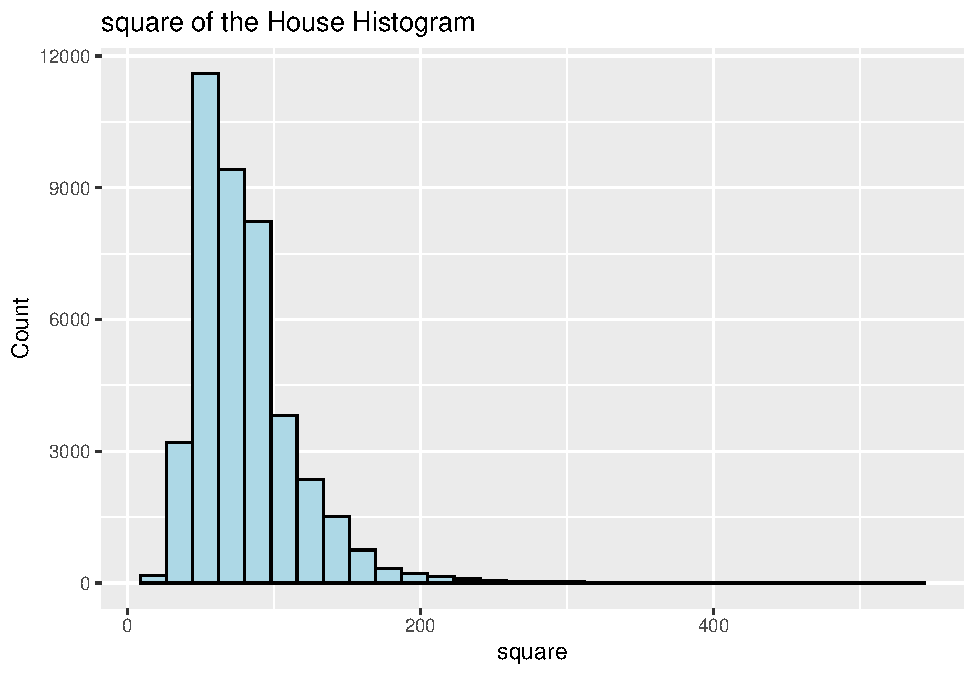
\includegraphics{Project_files/figure-latex/unnamed-chunk-17-1.pdf}

\begin{Shaded}
\begin{Highlighting}[]
\FunctionTok{mean}\NormalTok{(data2017}\SpecialCharTok{$}\NormalTok{square)}
\end{Highlighting}
\end{Shaded}

\begin{verbatim}
## [1] 80.9039
\end{verbatim}

\begin{Shaded}
\begin{Highlighting}[]
\FunctionTok{quantile}\NormalTok{(data2017}\SpecialCharTok{$}\NormalTok{square, }\FunctionTok{c}\NormalTok{(}\DecValTok{0}\NormalTok{, }\FloatTok{0.025}\NormalTok{, }\FloatTok{0.25}\NormalTok{, }\FloatTok{0.5}\NormalTok{, }\FloatTok{0.75}\NormalTok{, }\FloatTok{0.975}\NormalTok{, }\DecValTok{1}\NormalTok{))}
\end{Highlighting}
\end{Shaded}

\begin{verbatim}
##       0%     2.5%      25%      50%      75%    97.5%     100% 
##  15.0000  37.2725  57.3800  72.3600  95.0600 166.5900 532.2500
\end{verbatim}

A house with more 1745.5 square meter seems very unreasonable, so we
decided houses that are less than 1000 square meters are plausible.

\begin{Shaded}
\begin{Highlighting}[]
\NormalTok{data2017 }\OtherTok{\textless{}{-}}\NormalTok{ data2017 }\SpecialCharTok{\%\textgreater{}\%} 
  \FunctionTok{filter}\NormalTok{(square }\SpecialCharTok{\textless{}} \DecValTok{1000}\NormalTok{)}
\end{Highlighting}
\end{Shaded}

\hypertarget{bedroom}{%
\subsubsection{3.1.10 bedRoom}\label{bedroom}}

\hypertarget{might-be-a-report-error-move-the-house-with-0-bedroom-to-0-livingroom}{%
\subsection{might be a report error, move the house with 0 bedroom to 0
livingroom?}\label{might-be-a-report-error-move-the-house-with-0-bedroom-to-0-livingroom}}

One thing need to be noticed is that in this dataset, the variable
`livingRoom' could be understand as `bedroom' in the United States.
Thus, we decided to change the variable name from `livingRoom' to
`bedRoom'. The graph of number of bedrooms is unimodal, diamond-shaped,
and skews right. Most of the houses have 2 bedrooms, and the mean and
median number of bedrooms are both 2. Approximately 25\% of values are
below or equal to 1. Approximately 2.5\% of values are above 3.
(continued)

\begin{Shaded}
\begin{Highlighting}[]
\FunctionTok{ggplot}\NormalTok{(data2017, }\FunctionTok{aes}\NormalTok{(}\AttributeTok{x=}\NormalTok{bedRoom))}\SpecialCharTok{+}
  \FunctionTok{geom\_bar}\NormalTok{(}\AttributeTok{fill=}\StringTok{\textquotesingle{}lightblue\textquotesingle{}}\NormalTok{, }\AttributeTok{color=}\StringTok{\textquotesingle{}black\textquotesingle{}}\NormalTok{) }\SpecialCharTok{+} \CommentTok{\# use geom\_bar() instead of geom\_histogram()}
  \FunctionTok{xlab}\NormalTok{(}\StringTok{"bedRoom"}\NormalTok{)}\SpecialCharTok{+}\FunctionTok{ylab}\NormalTok{(}\StringTok{"Count"}\NormalTok{)}\SpecialCharTok{+}\FunctionTok{ggtitle}\NormalTok{(}\StringTok{"Number of bedroom Histogram"}\NormalTok{)}
\end{Highlighting}
\end{Shaded}

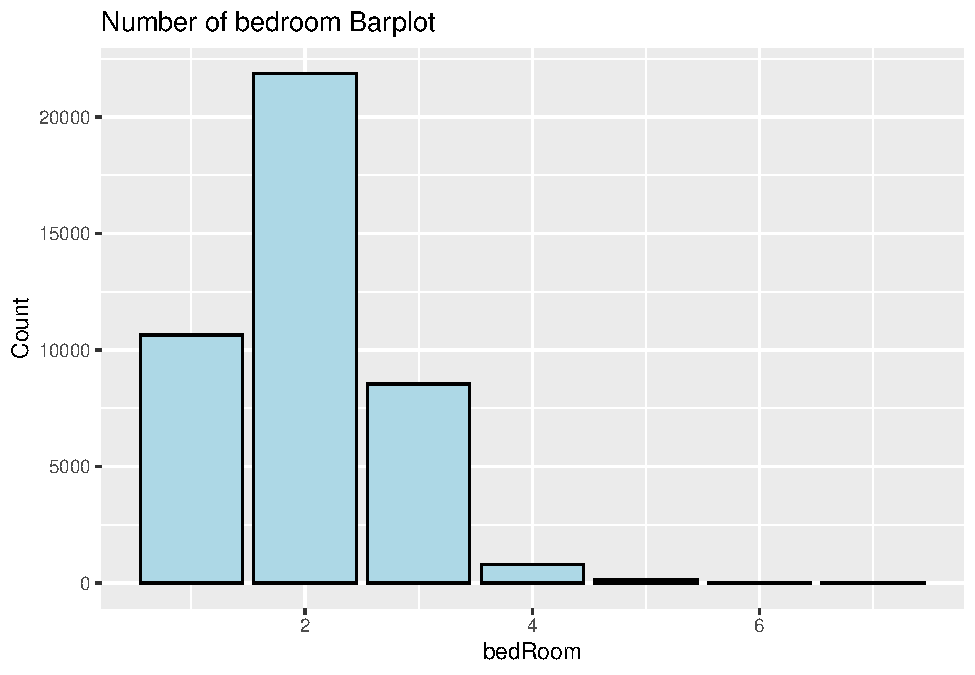
\includegraphics{Project_files/figure-latex/unnamed-chunk-19-1.pdf}

\begin{Shaded}
\begin{Highlighting}[]
\FunctionTok{mean}\NormalTok{(data2017}\SpecialCharTok{$}\NormalTok{bedRoom)}
\end{Highlighting}
\end{Shaded}

\begin{verbatim}
## [1] 2.000881
\end{verbatim}

\begin{Shaded}
\begin{Highlighting}[]
\FunctionTok{quantile}\NormalTok{(data2017}\SpecialCharTok{$}\NormalTok{bedRoom, }\FunctionTok{c}\NormalTok{(}\DecValTok{0}\NormalTok{, }\FloatTok{0.025}\NormalTok{, }\FloatTok{0.25}\NormalTok{, }\FloatTok{0.5}\NormalTok{, }\FloatTok{0.75}\NormalTok{, }\FloatTok{0.975}\NormalTok{, }\DecValTok{1}\NormalTok{))}
\end{Highlighting}
\end{Shaded}

\begin{verbatim}
##    0%  2.5%   25%   50%   75% 97.5%  100% 
##     0     1     1     2     2     3     7
\end{verbatim}

\begin{Shaded}
\begin{Highlighting}[]
\CommentTok{\# 1 house with 0 bed room}
\FunctionTok{table}\NormalTok{(data2017}\SpecialCharTok{$}\NormalTok{bedRoom)}
\end{Highlighting}
\end{Shaded}

\begin{verbatim}
## 
##     0     1     2     3     4     5     6     7 
##     1 10640 21859  8541   792   143    25     5
\end{verbatim}

\begin{Shaded}
\begin{Highlighting}[]
\NormalTok{data2017 }\SpecialCharTok{\%\textgreater{}\%}
  \FunctionTok{slice\_max}\NormalTok{(bedRoom,}\AttributeTok{n=}\DecValTok{1}\NormalTok{) }
\end{Highlighting}
\end{Shaded}

\begin{verbatim}
##             id DOM followers totalPrice price square bedRoom livingRoom kitchen
## 1 101100194821 257        77       2040 50000 408.00       7          3       1
## 2 101100882927 119        31       1690 52065 324.60       7          3       2
## 3 101100928521 251        94        700 20586 340.05       7          1       1
## 4 101101223183  17         5        840 58717 143.06       7          3       1
## 5 101101553400 100       168        678 24056 281.85       7          2       1
##   bathRoom constructionTime renovationCondition buildingStructure ladderRatio
## 1        3             2002                   4                 6       0.125
## 2        4             2001                   4                 6       0.250
## 3        2             2014                   2                 6       1.000
## 4        3             2011                   4                 6       0.500
## 5        3             2000                   4                 2       0.500
##   elevator fiveYearsProperty subway  district    month day totalFloor
## 1        0                 1      0   XiCheng February  28         24
## 2        1                 1      1  ChaoYang    March  24         22
## 3        1                 0      1    DaXing   August  13         24
## 4        1                 0      0 ChangPing    March  11          9
## 5        0                 1      0 ChangPing   August  14          6
##   floorRange
## 1        low
## 2     bottom
## 3     bottom
## 4     bottom
## 5     midium
\end{verbatim}

\begin{Shaded}
\begin{Highlighting}[]
\NormalTok{data2017 }\SpecialCharTok{\%\textgreater{}\%}
  \FunctionTok{slice\_min}\NormalTok{(bedRoom,}\AttributeTok{n=}\DecValTok{1}\NormalTok{)}
\end{Highlighting}
\end{Shaded}

\begin{verbatim}
##             id DOM followers totalPrice  price square bedRoom livingRoom
## 1 101101275312   3         0        450 145162     31       0          1
##   kitchen bathRoom constructionTime renovationCondition buildingStructure
## 1       1        1             2005                   1                 6
##   ladderRatio elevator fiveYearsProperty subway district month day totalFloor
## 1       0.081        1                 0      1  XiCheng March   6         10
##   floorRange
## 1     midium
\end{verbatim}

There is one house has 0 bedroom but sold in 145,612 yuan per square
meter which almost reached the highest square per meter sold among all
observations (150,000 yuan). Pulled out the link of this house, we found
that it is located in XiCheng. According to Lianjia website, this house
belongs to ``RongFeng 2008'' community. After a research on the
community, we found out that this is the average price per square meter
for this community. An investigation conducted by The Beijing News
indicates that ``RongFeng 2008'' has a relative 10,000 yuan higher price
per square meter compared with other communities in that area. But since
the houses in this community have very small areas, the total price is
still acceptable for most people who wanted to move to XiCheng. So this
house is not an outlier.

(\url{https://www.sohu.com/a/479132582_114988})

\begin{Shaded}
\begin{Highlighting}[]
\NormalTok{data }\SpecialCharTok{\%\textgreater{}\%}
  \FunctionTok{filter}\NormalTok{(id}\SpecialCharTok{==}\StringTok{"101101275312"}\NormalTok{)}
\end{Highlighting}
\end{Shaded}

\begin{verbatim}
##                                                  url           id      Lng
## 1 https://bj.lianjia.com/chengjiao/101101275312.html 101101275312 116.3432
##        Lat          Cid  tradeTime DOM followers totalPrice  price square
## 1 39.90053 1.111027e+12 2017-03-06   3         0        450 145162     31
##   livingRoom drawingRoom kitchen bathRoom floor buildingType constructionTime
## 1          0           1       1        1 中 10            1             2005
##   renovationCondition buildingStructure ladderRatio elevator fiveYearsProperty
## 1                   1                 6       0.081        1                 0
##   subway district communityAverage
## 1      1       10            92360
\end{verbatim}

\hypertarget{livingroom}{%
\subsubsection{3.1.11 livingRoom}\label{livingroom}}

The graph of number of living rooms is unimodal, diamond-shaped, and
skews right. The number of living rooms for all houses is between 0 to
4. Both the mean and median number of living rooms is 1. Approximately
2.5\% of values have no living room. Approximately 2.5\% of values have
more than 2 living rooms. Most houses sold in 2017 have 0 to 2 living
rooms and nearly 78\% of houses sold in 2017 have 1 living room. Houses
with 0 living room is the third greatest choice, and it is reasonable
for a house to have no living room, especially in the city.

\begin{Shaded}
\begin{Highlighting}[]
\FunctionTok{ggplot}\NormalTok{(data2017, }\FunctionTok{aes}\NormalTok{(}\AttributeTok{x=}\NormalTok{livingRoom))}\SpecialCharTok{+}
  \FunctionTok{geom\_bar}\NormalTok{(}\AttributeTok{fill=}\StringTok{\textquotesingle{}lightblue\textquotesingle{}}\NormalTok{, }\AttributeTok{color=}\StringTok{\textquotesingle{}black\textquotesingle{}}\NormalTok{) }\SpecialCharTok{+} \CommentTok{\# use geom\_bar() instead of geom\_histogram()}
  \FunctionTok{xlab}\NormalTok{(}\StringTok{"livingRoom"}\NormalTok{)}\SpecialCharTok{+}
  \FunctionTok{ylab}\NormalTok{(}\StringTok{"Count"}\NormalTok{)}\SpecialCharTok{+}
  \FunctionTok{ggtitle}\NormalTok{(}\StringTok{"Number of Living Rooms Histogram"}\NormalTok{)}
\end{Highlighting}
\end{Shaded}

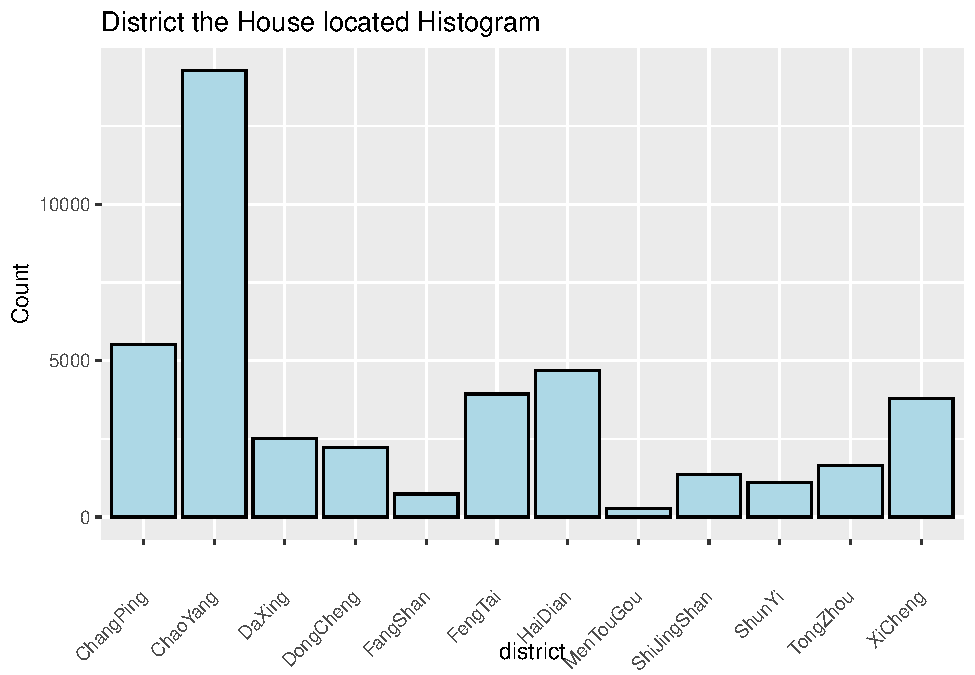
\includegraphics{Project_files/figure-latex/unnamed-chunk-21-1.pdf}

\begin{Shaded}
\begin{Highlighting}[]
\FunctionTok{mean}\NormalTok{(data2017}\SpecialCharTok{$}\NormalTok{livingRoom)}
\end{Highlighting}
\end{Shaded}

\begin{verbatim}
## [1] 1.09232
\end{verbatim}

\begin{Shaded}
\begin{Highlighting}[]
\FunctionTok{quantile}\NormalTok{(data2017}\SpecialCharTok{$}\NormalTok{livingRoom, }\FunctionTok{c}\NormalTok{(}\DecValTok{0}\NormalTok{, }\FloatTok{0.025}\NormalTok{, }\FloatTok{0.25}\NormalTok{, }\FloatTok{0.5}\NormalTok{, }\FloatTok{0.75}\NormalTok{, }\FloatTok{0.975}\NormalTok{, }\DecValTok{1}\NormalTok{))}
\end{Highlighting}
\end{Shaded}

\begin{verbatim}
##    0%  2.5%   25%   50%   75% 97.5%  100% 
##     0     0     1     1     1     2     4
\end{verbatim}

\begin{Shaded}
\begin{Highlighting}[]
\FunctionTok{table}\NormalTok{(data2017}\SpecialCharTok{$}\NormalTok{livingRoom)}\SpecialCharTok{/}\FunctionTok{length}\NormalTok{(data2017}\SpecialCharTok{$}\NormalTok{livingRoom)}
\end{Highlighting}
\end{Shaded}

\begin{verbatim}
## 
##            0            1            2            3            4 
## 0.0608722563 0.7888634957 0.1474789316 0.0026424796 0.0001428367
\end{verbatim}

\hypertarget{district-categorical}{%
\subsubsection{3.1.12 district
(Categorical)}\label{district-categorical}}

\begin{Shaded}
\begin{Highlighting}[]
\FunctionTok{ggplot}\NormalTok{(data2017, }\FunctionTok{aes}\NormalTok{(}\AttributeTok{x=}\NormalTok{district))}\SpecialCharTok{+}
  \FunctionTok{geom\_bar}\NormalTok{(}\AttributeTok{fill=}\StringTok{\textquotesingle{}lightblue\textquotesingle{}}\NormalTok{, }\AttributeTok{color=}\StringTok{\textquotesingle{}black\textquotesingle{}}\NormalTok{) }\SpecialCharTok{+}
  \FunctionTok{theme}\NormalTok{(}\AttributeTok{axis.text.x =} \FunctionTok{element\_text}\NormalTok{(}\AttributeTok{angle =} \DecValTok{90}\NormalTok{, }\AttributeTok{vjust =} \FloatTok{0.5}\NormalTok{, }\AttributeTok{hjust=}\DecValTok{1}\NormalTok{))}\SpecialCharTok{+}
  \FunctionTok{ggtitle}\NormalTok{(}\StringTok{"District the House located Histogram"}\NormalTok{) }
\end{Highlighting}
\end{Shaded}

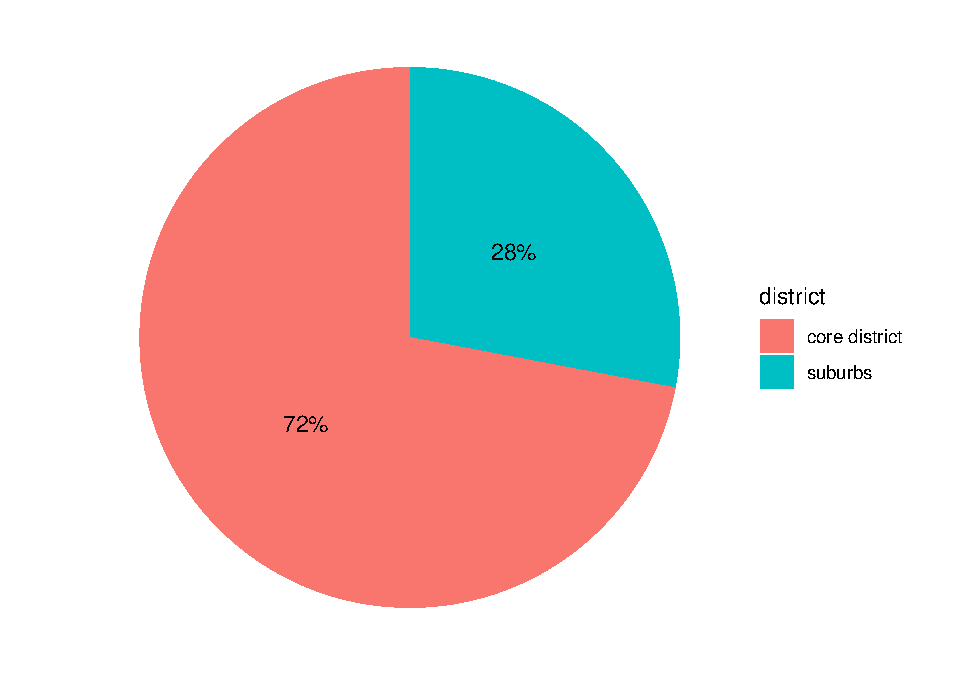
\includegraphics{Project_files/figure-latex/unnamed-chunk-22-1.pdf}

\begin{Shaded}
\begin{Highlighting}[]
\NormalTok{district\_percentage }\OtherTok{\textless{}{-}}\NormalTok{ data2017 }\SpecialCharTok{\%\textgreater{}\%}
  \FunctionTok{group\_by}\NormalTok{(district) }\SpecialCharTok{\%\textgreater{}\%}
  \FunctionTok{count}\NormalTok{(district) }\SpecialCharTok{\%\textgreater{}\%} \CommentTok{\# number of houses sold in each district}
  \FunctionTok{mutate}\NormalTok{(}\AttributeTok{percentage=}\NormalTok{n}\SpecialCharTok{*}\DecValTok{100}\SpecialCharTok{/}\DecValTok{42004}\NormalTok{) }\SpecialCharTok{\%\textgreater{}\%} \CommentTok{\# what percentage of sold houses are in each district}
  \FunctionTok{arrange}\NormalTok{(}\FunctionTok{desc}\NormalTok{(n))}
\NormalTok{district\_percentage}
\end{Highlighting}
\end{Shaded}

\begin{verbatim}
## # A tibble: 13 x 3
## # Groups:   district [13]
##    district        n percentage
##    <chr>       <int>      <dbl>
##  1 ChaoYang    14282     34.0  
##  2 ChangPing    5509     13.1  
##  3 HaiDian      4681     11.1  
##  4 FengTai      3931      9.36 
##  5 XiCheng      3777      8.99 
##  6 DongCheng    2223      5.29 
##  7 DaXing       2162      5.15 
##  8 TongZhou     1652      3.93 
##  9 ShiJingShan  1356      3.23 
## 10 ShunYi       1096      2.61 
## 11 FangShan      730      1.74 
## 12 YiZhuang      348      0.828
## 13 MenTouGou     259      0.617
\end{verbatim}

\hypertarget{kitchen}{%
\subsubsection{3.1.13 kitchen}\label{kitchen}}

\begin{Shaded}
\begin{Highlighting}[]
\NormalTok{data2017 }\SpecialCharTok{\%\textgreater{}\%} 
  \FunctionTok{filter}\NormalTok{(kitchen }\SpecialCharTok{\textgreater{}} \DecValTok{2}\NormalTok{) }
\end{Highlighting}
\end{Shaded}

\begin{verbatim}
##             id DOM followers totalPrice price square bedRoom livingRoom kitchen
## 1 101101782929  69        78        735 26750 274.77       4          2       3
##   bathRoom constructionTime renovationCondition buildingStructure ladderRatio
## 1        2             2001                   4                 6         0.5
##   elevator fiveYearsProperty subway  district     month day totalFloor
## 1        1                 1      1 ChangPing September  13         13
##   floorRange
## 1       high
\end{verbatim}

There are two houses with more than 2 kitchens, which seem odd. Taking a
closer look, both of these houses had less than 300 square meters, which
is impossible to have 3 kitchens in fairly medium house size. Therefore,
we removed these two outliers.

\begin{Shaded}
\begin{Highlighting}[]
\NormalTok{data2017 }\OtherTok{\textless{}{-}}\NormalTok{ data2017 }\SpecialCharTok{\%\textgreater{}\%}
  \FunctionTok{filter}\NormalTok{(kitchen }\SpecialCharTok{\textless{}} \DecValTok{3}\NormalTok{)}
\end{Highlighting}
\end{Shaded}

The distribution for the number of kitchens shows that most listings
have only one kitchen in their property. However, having no kitchen is
evidently more common than having 2 kitchens in a property.

\begin{Shaded}
\begin{Highlighting}[]
\FunctionTok{ggplot}\NormalTok{(data2017, }\FunctionTok{aes}\NormalTok{(}\AttributeTok{x =}\NormalTok{ kitchen)) }\SpecialCharTok{+}
  \FunctionTok{geom\_bar}\NormalTok{(}\AttributeTok{fill =} \StringTok{"lightblue"}\NormalTok{) }\SpecialCharTok{+}
  \FunctionTok{ggtitle}\NormalTok{(}\StringTok{"Kitchen Summary"}\NormalTok{) }\SpecialCharTok{+}
  \FunctionTok{xlab}\NormalTok{(}\StringTok{"Number of Kitchens"}\NormalTok{) }\SpecialCharTok{+}
  \FunctionTok{ylab}\NormalTok{(}\StringTok{"Count"}\NormalTok{)}
\end{Highlighting}
\end{Shaded}

\includegraphics{Project_files/figure-latex/unnamed-chunk-25-1.pdf}

\hypertarget{bathroom}{%
\subsubsection{3.1.14 bathroom}\label{bathroom}}

The distribution for the number of bathrooms shows that most listings
have only one bathroom in their property. This distribution skews
heavily to the right and the count decreases as number of bathrooms
increases.

\begin{Shaded}
\begin{Highlighting}[]
\FunctionTok{ggplot}\NormalTok{(data2017, }\FunctionTok{aes}\NormalTok{(}\AttributeTok{x =}\NormalTok{ bathRoom)) }\SpecialCharTok{+}
  \FunctionTok{geom\_bar}\NormalTok{(}\AttributeTok{fill =} \StringTok{"lightblue"}\NormalTok{) }\SpecialCharTok{+}
  \FunctionTok{ggtitle}\NormalTok{(}\StringTok{"Bathroom Summary"}\NormalTok{) }\SpecialCharTok{+}
  \FunctionTok{xlab}\NormalTok{(}\StringTok{"Number of Bathrooms"}\NormalTok{) }\SpecialCharTok{+}
  \FunctionTok{ylab}\NormalTok{(}\StringTok{"Count"}\NormalTok{)}
\end{Highlighting}
\end{Shaded}

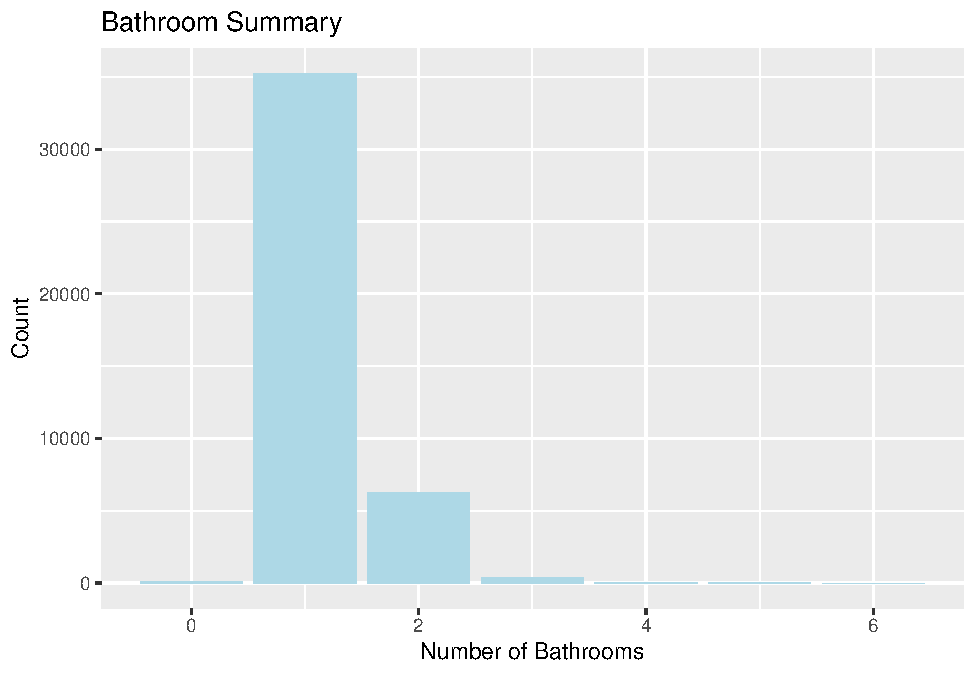
\includegraphics{Project_files/figure-latex/unnamed-chunk-26-1.pdf}

\hypertarget{construction-time}{%
\subsubsection{3.1.15 construction time}\label{construction-time}}

\begin{Shaded}
\begin{Highlighting}[]
\FunctionTok{table}\NormalTok{(data2017}\SpecialCharTok{$}\NormalTok{constructionTime)}
\end{Highlighting}
\end{Shaded}

\begin{verbatim}
## 
## 1950 1952 1953 1954 1955 1956 1957 1958 1959 1960 1961 1962 1963 1964 1965 1966 
##    1    1    2    9    6    9   10   21   13   31    2    5   16   23   35   22 
## 1967 1968 1969 1970 1971 1972 1973 1974 1975 1976 1977 1978 1979 1980 1981 1982 
##    6    2    1   63    2    5   22   30   49   68   66  130  224  547  330  396 
## 1983 1984 1985 1986 1987 1988 1989 1990 1991 1992 1993 1994 1995 1996 1997 1998 
##  424  488  640  679  736  790  778 1151  647 1162  965 1142 1217 1215  911 1371 
## 1999 2000 2001 2002 2003 2004 2005 2006 2007 2008 2009 2010 2011 2012 2013 2014 
## 1276 1801 1351 1497 2284 2525 2425 1888 1780 1740 1798 1430 1000 1043  626  781 
## 2015 2016 
##  259   38
\end{verbatim}

\begin{Shaded}
\begin{Highlighting}[]
\FunctionTok{median}\NormalTok{(data2017}\SpecialCharTok{$}\NormalTok{constructionTime)}
\end{Highlighting}
\end{Shaded}

\begin{verbatim}
## [1] 2002
\end{verbatim}

\begin{Shaded}
\begin{Highlighting}[]
\FunctionTok{mean}\NormalTok{(data2017}\SpecialCharTok{$}\NormalTok{constructionTime)}
\end{Highlighting}
\end{Shaded}

\begin{verbatim}
## [1] 1999.547
\end{verbatim}

The year of construction of the listings that were transacted in 2017
ranges from the year 1950 to the year 2016. Out of all the included
listings, most of the properties were built in the year 2004
accumulating a total of 2525 properties.

The distribution skews to the left as the median of the year 2002 and
mean of the year 1999 both lie to the left of the mode of the year 2004.

\begin{Shaded}
\begin{Highlighting}[]
\FunctionTok{ggplot}\NormalTok{(data2017, }\FunctionTok{aes}\NormalTok{(}\AttributeTok{x =}\NormalTok{ constructionTime)) }\SpecialCharTok{+}
  \FunctionTok{geom\_bar}\NormalTok{(}\AttributeTok{fill =} \StringTok{"lightblue"}\NormalTok{) }\SpecialCharTok{+}
  \FunctionTok{ggtitle}\NormalTok{(}\StringTok{"Time of Construction Summary"}\NormalTok{) }\SpecialCharTok{+}
  \FunctionTok{xlab}\NormalTok{(}\StringTok{"Time of Construction"}\NormalTok{) }\SpecialCharTok{+}
  \FunctionTok{ylab}\NormalTok{(}\StringTok{"Count"}\NormalTok{)}
\end{Highlighting}
\end{Shaded}

\includegraphics{Project_files/figure-latex/unnamed-chunk-29-1.pdf}

\hypertarget{renovation-condition}{%
\subsubsection{3.1.16 renovation condition}\label{renovation-condition}}

The condition of renovation

The distribution for the condition of renovation shows that most
listings have the highest score of 4 in terms of the condition of
renovation for their listing. This distribution skews heavily to the
left.

\begin{Shaded}
\begin{Highlighting}[]
\FunctionTok{ggplot}\NormalTok{(data2017, }\FunctionTok{aes}\NormalTok{(}\AttributeTok{x =}\NormalTok{ renovationCondition)) }\SpecialCharTok{+}
  \FunctionTok{geom\_bar}\NormalTok{(}\AttributeTok{fill =} \StringTok{"lightblue"}\NormalTok{) }\SpecialCharTok{+}
  \FunctionTok{ggtitle}\NormalTok{(}\StringTok{"Condition of Renovation Summary"}\NormalTok{) }\SpecialCharTok{+}
  \FunctionTok{xlab}\NormalTok{(}\StringTok{"Condition of Renovation"}\NormalTok{) }\SpecialCharTok{+}
  \FunctionTok{ylab}\NormalTok{(}\StringTok{"Count"}\NormalTok{)}
\end{Highlighting}
\end{Shaded}

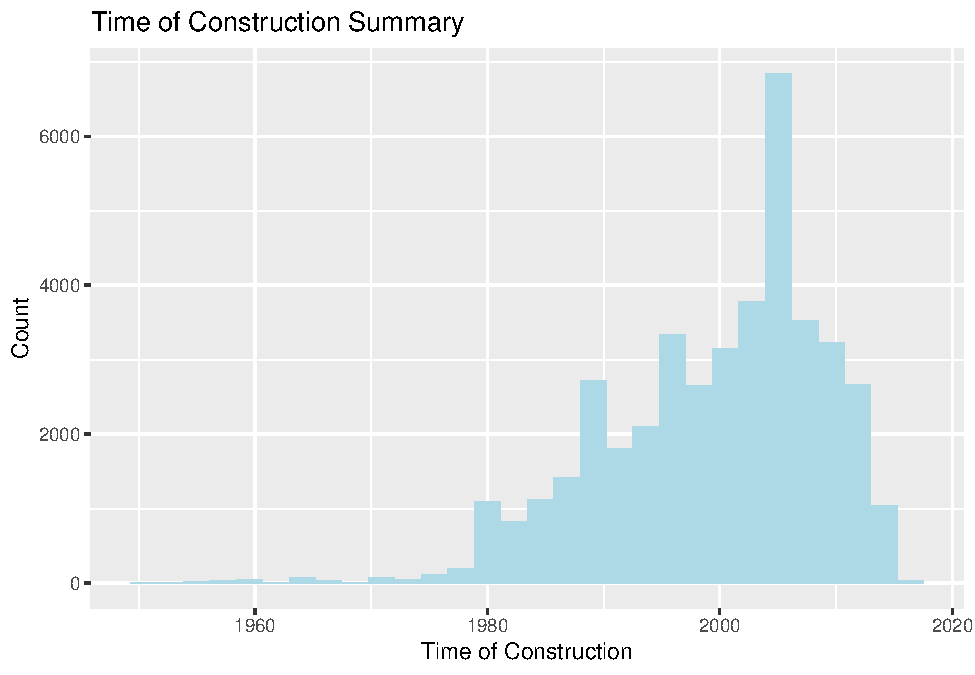
\includegraphics{Project_files/figure-latex/unnamed-chunk-30-1.pdf}

\hypertarget{building-structure}{%
\subsubsection{3.1.17 building structure}\label{building-structure}}

The distribution for the building structure shows that most listings are
made of steel-concrete composite. This distribution skews heavily to the
left.

\begin{Shaded}
\begin{Highlighting}[]
\FunctionTok{ggplot}\NormalTok{(data2017, }\FunctionTok{aes}\NormalTok{(}\AttributeTok{x =}\NormalTok{ buildingStructure)) }\SpecialCharTok{+}
  \FunctionTok{geom\_bar}\NormalTok{(}\AttributeTok{fill =} \StringTok{"lightblue"}\NormalTok{) }\SpecialCharTok{+}
  \FunctionTok{ggtitle}\NormalTok{(}\StringTok{"Structure of Building Summary"}\NormalTok{) }\SpecialCharTok{+}
  \FunctionTok{xlab}\NormalTok{(}\StringTok{"Structure of Building"}\NormalTok{) }\SpecialCharTok{+}
  \FunctionTok{ylab}\NormalTok{(}\StringTok{"Count"}\NormalTok{)}
\end{Highlighting}
\end{Shaded}

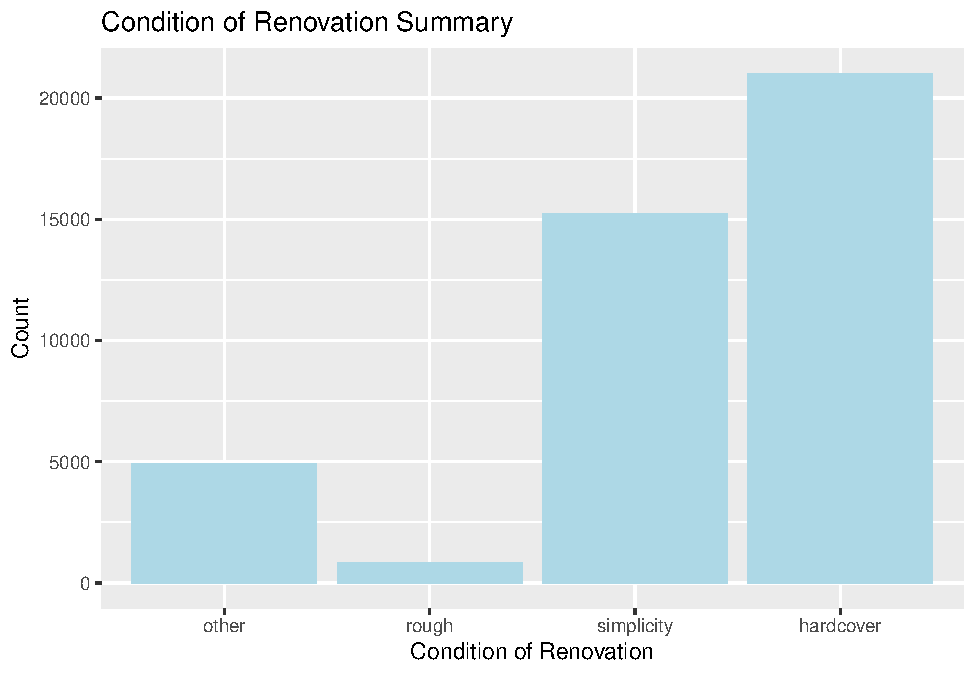
\includegraphics{Project_files/figure-latex/unnamed-chunk-31-1.pdf}

\hypertarget{ladder-ratio}{%
\subsubsection{3.1.18 ladder ratio}\label{ladder-ratio}}

The maximum value for ladderRatio is 10009400, which seems like a typo,
so we decided to remove this observation.

\begin{Shaded}
\begin{Highlighting}[]
\NormalTok{data2017 }\OtherTok{\textless{}{-}}\NormalTok{ data2017 }\SpecialCharTok{\%\textgreater{}\%} 
  \FunctionTok{filter}\NormalTok{(ladderRatio }\SpecialCharTok{\textless{}} \DecValTok{5}\NormalTok{)}
\end{Highlighting}
\end{Shaded}

\begin{Shaded}
\begin{Highlighting}[]
\FunctionTok{table}\NormalTok{(data2017}\SpecialCharTok{$}\NormalTok{ladderRatio)}
\end{Highlighting}
\end{Shaded}

\begin{verbatim}
## 
## 0.014 0.015  0.02 0.022 0.023 0.025 0.026 0.028 0.029  0.03 0.031 0.033 0.034 
##    10     2    18     3     2     1     2     9     3     2     6    12     1 
## 0.035 0.036 0.037 0.038 0.039  0.04 0.041 0.042 0.043 0.045 0.047 0.048  0.05 
##     2     8     1    12     3     6     1    11     4     7     5     8    18 
## 0.053 0.054 0.056 0.057 0.059  0.06 0.061 0.062 0.065 0.067 0.069 0.071 0.074 
##     9     8    11    15    64     1    13    19     6    14     4    24     5 
## 0.075 0.077  0.08 0.081 0.083 0.086 0.087 0.088 0.091 0.095 0.098   0.1 0.103 
##     1    35     9     9    42    20    39     1    46    14    16   109    38 
## 0.105 0.107 0.108 0.111 0.114 0.118  0.12 0.121 0.125 0.129  0.13 0.133 0.136 
##    31    11     6   191     1    42    29    18   406    10    31    37    25 
## 0.138 0.143 0.148  0.15 0.154 0.156 0.158  0.16 0.161 0.162 0.167 0.171 0.174 
##    19   377    16    26   128     1    31     7    12    13   929     5    62 
## 0.176 0.179 0.182 0.185 0.188 0.189  0.19 0.192 0.198   0.2 0.208 0.211 0.214 
##    40     2   204     1    66     1    41    19     3  1842     2    59   182 
## 0.217 0.222 0.227 0.231 0.235 0.238  0.24  0.25 0.255 0.261 0.263 0.267 0.273 
##    11   514    15   124    45     1     2  5735     1    11    21    14   221 
## 0.276 0.278 0.286   0.3 0.304 0.308 0.312 0.318 0.333 0.345 0.346 0.353 0.364 
##     2     9   963   847    13     5     3     2  9242     9     7     1    37 
##  0.37 0.375 0.385   0.4 0.417 0.429 0.438 0.444 0.467   0.5 0.538 0.571 0.583 
##    12   618    16  1009     1    76     2    56     1 14602     2     6     2 
##   0.6 0.625 0.667 0.714  0.75   0.8 0.818 0.833  0.87 0.889     1  1.25 1.333 
##    18     7  1184     1    45     3     1     2     3     3   724     2    21 
##   1.5 1.667     2     3 
##    54     1    21     1
\end{verbatim}

\begin{Shaded}
\begin{Highlighting}[]
\FunctionTok{median}\NormalTok{(data2017}\SpecialCharTok{$}\NormalTok{ladderRatio)}
\end{Highlighting}
\end{Shaded}

\begin{verbatim}
## [1] 0.333
\end{verbatim}

\begin{Shaded}
\begin{Highlighting}[]
\FunctionTok{mean}\NormalTok{(data2017}\SpecialCharTok{$}\NormalTok{ladderRatio)}
\end{Highlighting}
\end{Shaded}

\begin{verbatim}
## [1] 0.3797018
\end{verbatim}

The distribution for the ladder ratio shows that most listings have 2
residents to one elevator per floor. This distribution skews heavily to
the left as the average number of residents sharing an elevator per
floor is 3.

\begin{Shaded}
\begin{Highlighting}[]
\FunctionTok{ggplot}\NormalTok{(data2017, }\FunctionTok{aes}\NormalTok{(}\AttributeTok{x =}\NormalTok{ ladderRatio)) }\SpecialCharTok{+}
  \FunctionTok{geom\_bar}\NormalTok{(}\AttributeTok{fill =} \StringTok{"lightblue"}\NormalTok{, }\AttributeTok{width =} \FloatTok{0.05}\NormalTok{) }\SpecialCharTok{+}
  \FunctionTok{ggtitle}\NormalTok{(}\StringTok{"Ladder Ratio Summary"}\NormalTok{) }\SpecialCharTok{+}
  \FunctionTok{xlab}\NormalTok{(}\StringTok{"Ladder Ratio"}\NormalTok{) }\SpecialCharTok{+}
  \FunctionTok{ylab}\NormalTok{(}\StringTok{"Count"}\NormalTok{)}
\end{Highlighting}
\end{Shaded}

\begin{verbatim}
## Warning: position_stack requires non-overlapping x intervals
\end{verbatim}

\includegraphics{Project_files/figure-latex/unnamed-chunk-35-1.pdf}

\hypertarget{elevator}{%
\subsubsection{3.1.19 elevator}\label{elevator}}

The distribution for the presence of an elevator shows that it is more
common for listings to have at lease one elevator in the building
compared to none at all.

\begin{Shaded}
\begin{Highlighting}[]
\FunctionTok{ggplot}\NormalTok{(data2017, }\FunctionTok{aes}\NormalTok{(}\AttributeTok{x =}\NormalTok{ elevator)) }\SpecialCharTok{+}
  \FunctionTok{geom\_bar}\NormalTok{(}\AttributeTok{fill =} \StringTok{"lightblue"}\NormalTok{) }\SpecialCharTok{+}
  \FunctionTok{ggtitle}\NormalTok{(}\StringTok{"Availability of Elevator"}\NormalTok{) }\SpecialCharTok{+}
  \FunctionTok{xlab}\NormalTok{(}\StringTok{"Elevator"}\NormalTok{) }\SpecialCharTok{+}
  \FunctionTok{ylab}\NormalTok{(}\StringTok{"Count"}\NormalTok{)}
\end{Highlighting}
\end{Shaded}

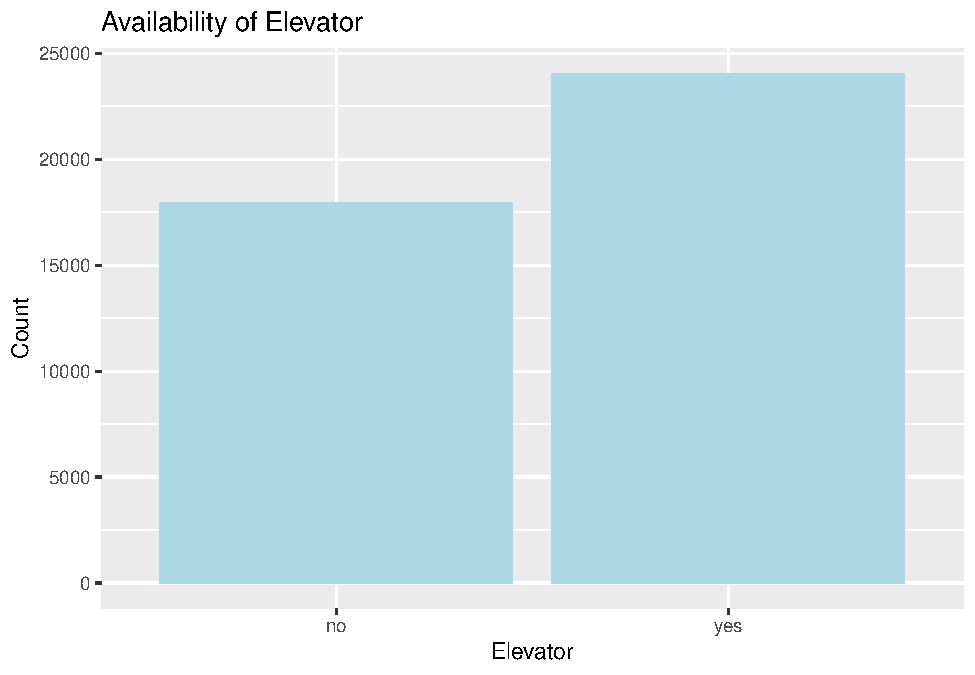
\includegraphics{Project_files/figure-latex/unnamed-chunk-36-1.pdf}

\hypertarget{five-years-property}{%
\subsubsection{3.1.20 five years property}\label{five-years-property}}

The distribution for whether the previous has stayed in the listing for
less than five years shows that most sellers stay in their property for
less than five years.

\begin{Shaded}
\begin{Highlighting}[]
\FunctionTok{ggplot}\NormalTok{(data2017, }\FunctionTok{aes}\NormalTok{(}\AttributeTok{x =}\NormalTok{ fiveYearsProperty)) }\SpecialCharTok{+}
  \FunctionTok{geom\_bar}\NormalTok{(}\AttributeTok{fill =} \StringTok{"lightblue"}\NormalTok{) }\SpecialCharTok{+}
  \FunctionTok{ggtitle}\NormalTok{(}\StringTok{"Five Years Property Summary"}\NormalTok{) }\SpecialCharTok{+}
  \FunctionTok{xlab}\NormalTok{(}\StringTok{"Five Years Property"}\NormalTok{) }\SpecialCharTok{+}
  \FunctionTok{ylab}\NormalTok{(}\StringTok{"Count"}\NormalTok{)}
\end{Highlighting}
\end{Shaded}

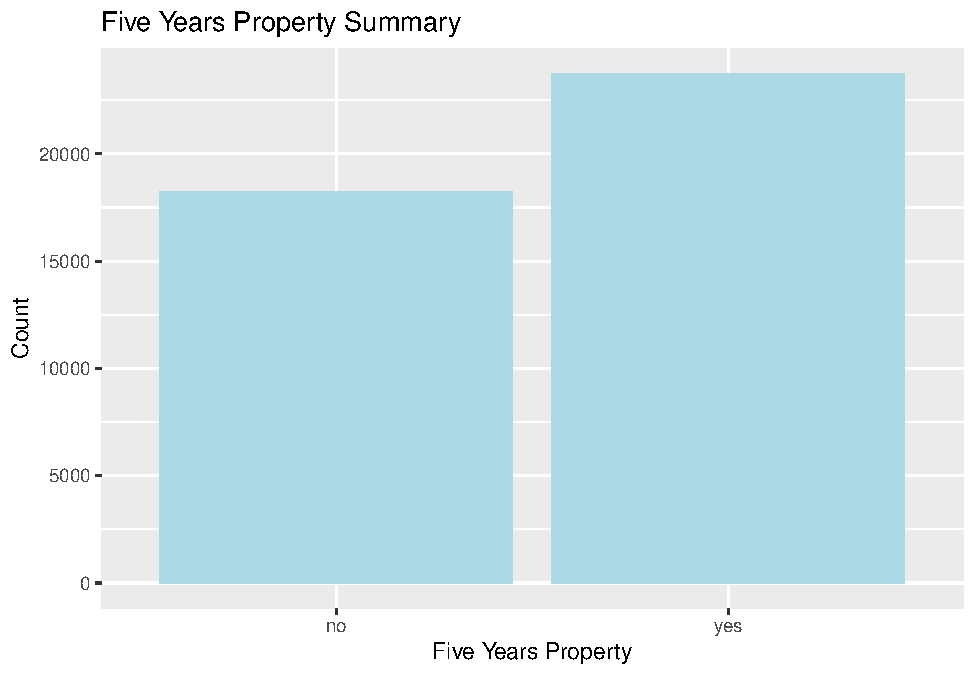
\includegraphics{Project_files/figure-latex/unnamed-chunk-37-1.pdf}

\hypertarget{subway}{%
\subsubsection{3.1.21 subway}\label{subway}}

The distribution for the presence of any nearby subways shows that it is
more common for listings to have at lease one subway nearby the building
compared to none at all.

\begin{Shaded}
\begin{Highlighting}[]
\FunctionTok{ggplot}\NormalTok{(data2017, }\FunctionTok{aes}\NormalTok{(}\AttributeTok{x =}\NormalTok{ subway)) }\SpecialCharTok{+}
  \FunctionTok{geom\_bar}\NormalTok{(}\AttributeTok{fill =} \StringTok{"lightblue"}\NormalTok{) }\SpecialCharTok{+}
  \FunctionTok{ggtitle}\NormalTok{(}\StringTok{"Subway Summary"}\NormalTok{) }\SpecialCharTok{+}
  \FunctionTok{xlab}\NormalTok{(}\StringTok{"Availability of Nearby Subways"}\NormalTok{) }\SpecialCharTok{+}
  \FunctionTok{ylab}\NormalTok{(}\StringTok{"Count"}\NormalTok{)}
\end{Highlighting}
\end{Shaded}

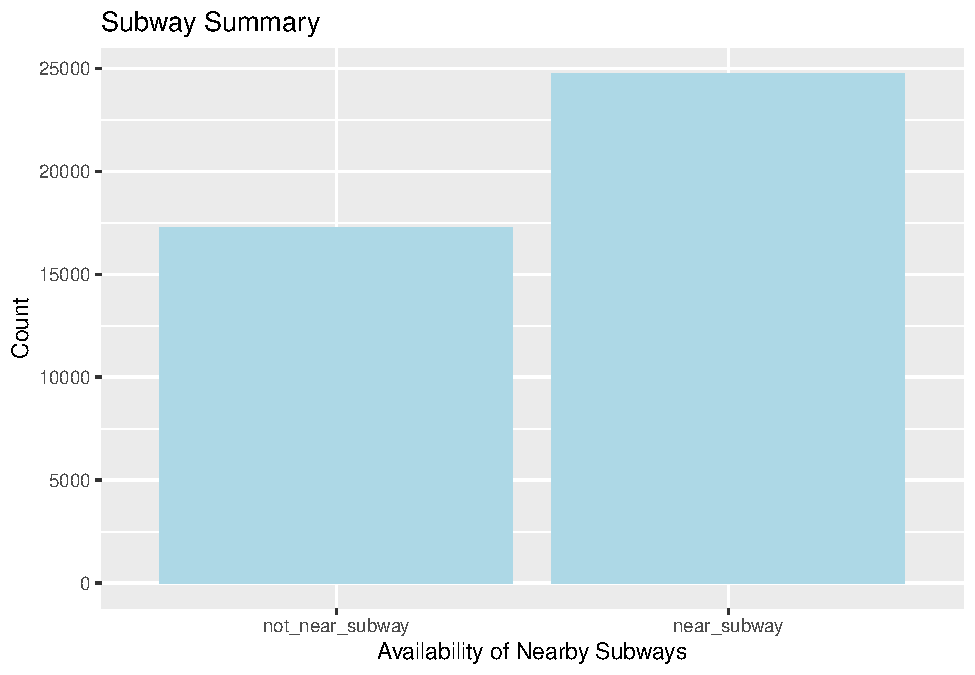
\includegraphics{Project_files/figure-latex/unnamed-chunk-38-1.pdf}

\hypertarget{potential-relationships-between-variables}{%
\subsection{3.2 Potential Relationships between
Variables}\label{potential-relationships-between-variables}}

\hypertarget{dom-vs.-followers}{%
\subsubsection{3.2.1 DOM vs.~followers}\label{dom-vs.-followers}}

\emph{Do houses sold fast have many followers?} Among these 474 houses
that were sold within 1 day, 376 have no follower and the maximum number
of followers is 39, which is not a significant number of followers. But
in general as shown on the graph, the graph is unimodal, diamond-shaped,
and heavily skew right. Which indicates that the number of followers is
decreasing as the number of days on market increase.

\begin{Shaded}
\begin{Highlighting}[]
\FunctionTok{table}\NormalTok{(data2017}\SpecialCharTok{$}\NormalTok{DOM}\SpecialCharTok{\textless{}=}\DecValTok{1}\NormalTok{) }\CommentTok{\# number of 0 or 1 Days in market}
\end{Highlighting}
\end{Shaded}

\begin{verbatim}
## 
## FALSE  TRUE 
## 41530   474
\end{verbatim}

\begin{Shaded}
\begin{Highlighting}[]
\NormalTok{data2017 }\SpecialCharTok{\%\textgreater{}\%}
  \FunctionTok{filter}\NormalTok{(DOM}\SpecialCharTok{\textless{}=}\DecValTok{1}\NormalTok{) }\SpecialCharTok{\%\textgreater{}\%}
  \FunctionTok{count}\NormalTok{(followers) }\CommentTok{\# Do houses sold fast have many followers?}
\end{Highlighting}
\end{Shaded}

\begin{verbatim}
##    followers   n
## 1          0 376
## 2          1  20
## 3          2  13
## 4          3   8
## 5          4  10
## 6          5   6
## 7          6   5
## 8          7   3
## 9          8   3
## 10         9   6
## 11        10   2
## 12        11   1
## 13        12   4
## 14        13   3
## 15        14   4
## 16        16   2
## 17        19   1
## 18        20   2
## 19        21   1
## 20        23   1
## 21        25   1
## 22        32   1
## 23        39   1
\end{verbatim}

\begin{Shaded}
\begin{Highlighting}[]
\FunctionTok{ggplot}\NormalTok{(data2017, }\FunctionTok{aes}\NormalTok{(}\AttributeTok{x=}\NormalTok{DOM,}\AttributeTok{y=}\NormalTok{followers))}\SpecialCharTok{+}
  \FunctionTok{geom\_col}\NormalTok{(}\AttributeTok{fill=}\StringTok{"lightblue"}\NormalTok{)}
\end{Highlighting}
\end{Shaded}

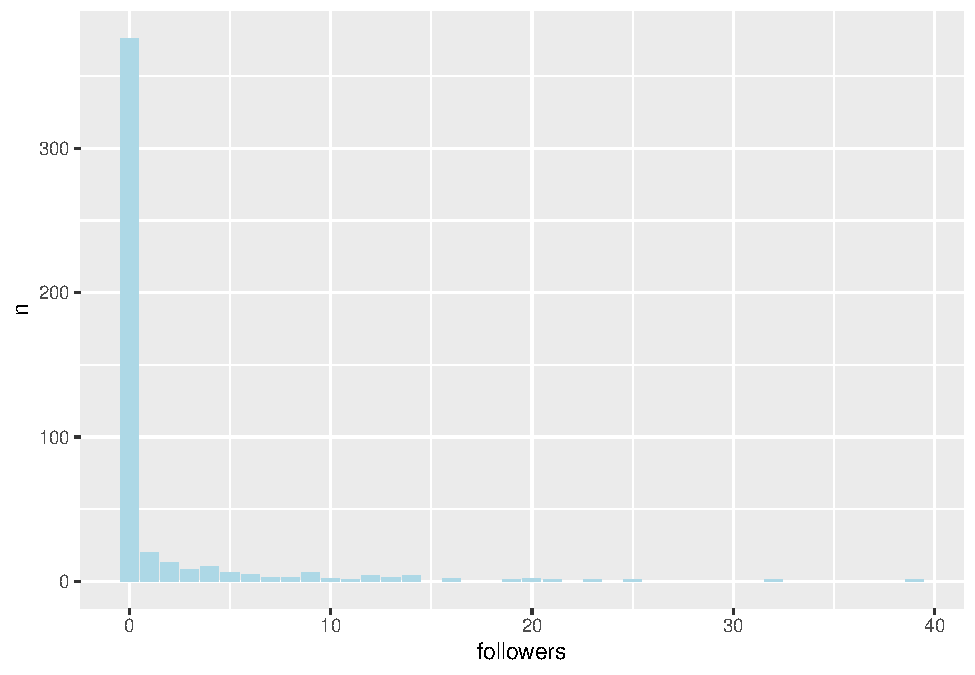
\includegraphics{Project_files/figure-latex/unnamed-chunk-39-1.pdf}

\hypertarget{dom-vs.-price}{%
\subsubsection{3.2.2 DOM vs.~price}\label{dom-vs.-price}}

\hypertarget{price-vs.-construction-time}{%
\subsubsection{3.2.3 price vs.~construction
time}\label{price-vs.-construction-time}}

\hypertarget{construction-time-vs.-renovation-condition}{%
\subsubsection{3.2.4 construction time vs.~renovation
condition}\label{construction-time-vs.-renovation-condition}}

\hypertarget{construction-time-vs.-building-structure}{%
\subsubsection{3.2.5 construction time vs.~building
structure}\label{construction-time-vs.-building-structure}}

\hypertarget{district-vs.-square}{%
\subsubsection{3.2.6 district vs.~square}\label{district-vs.-square}}

\emph{Districts that have most large \& small houses sold}

(ChaoYang(7) has significantly highest amount of these. But one
surprising observation is that ChangPing(6) has the second highest
amounts of houses in the higher 2.5\%. ChangPing indeed has a relative
large area compared with other districts in Beijing but it is relative
far from the core area of the city. Thus, it is reasonable to have great
proportion of houses sold with large square meters with lower than
average square meters price.)

As indicated under the `square' variable, the top 2.5\% of houses sold
have area over 167 square meters. Let's define houses over 167 square
meters as ``large houses''. Then ChaoYang has the significantly highest
amounts of large houses. ChangPing has the second highest amounts.

The bottom 2.5\% of houses sold have less than 37 square meters. Let's
define houses less than 37 square meters as ``small houses''.
Surprisingly, ChangPing also has the greatest amounts of small houses
sold in 2017. And then second one is ChaoYang.

Let's compare the total amounts of houses sold in ChaoYang and
ChangPing. Let's then compare the total areas of ChaoYang and ChangPing.

\begin{Shaded}
\begin{Highlighting}[]
\NormalTok{data2017}\SpecialCharTok{\%\textgreater{}\%}
  \FunctionTok{filter}\NormalTok{(square}\SpecialCharTok{\textgreater{}=}\DecValTok{167}\NormalTok{) }\SpecialCharTok{\%\textgreater{}\%} \CommentTok{\# top 2.5\% large houses}
  \FunctionTok{count}\NormalTok{(district)}
\end{Highlighting}
\end{Shaded}

\begin{verbatim}
##       district   n
## 1    ChangPing 196
## 2     ChaoYang 448
## 3       DaXing  41
## 4    DongCheng  55
## 5     FangShan   4
## 6      FengTai  47
## 7      HaiDian 115
## 8  ShiJingShan  11
## 9       ShunYi  39
## 10    TongZhou  11
## 11     XiCheng  44
## 12    YiZhuang  21
\end{verbatim}

\begin{Shaded}
\begin{Highlighting}[]
\NormalTok{data2017}\SpecialCharTok{\%\textgreater{}\%}
  \FunctionTok{filter}\NormalTok{(square}\SpecialCharTok{\textless{}=}\DecValTok{37}\NormalTok{) }\SpecialCharTok{\%\textgreater{}\%} \CommentTok{\# bottom 2.5\% small houses}
  \FunctionTok{count}\NormalTok{(district)}
\end{Highlighting}
\end{Shaded}

\begin{verbatim}
##       district   n
## 1    ChangPing 204
## 2     ChaoYang 159
## 3       DaXing   5
## 4    DongCheng  75
## 5     FangShan   5
## 6      FengTai 119
## 7      HaiDian  54
## 8  ShiJingShan  14
## 9       ShunYi 108
## 10    TongZhou  25
## 11     XiCheng 225
## 12    YiZhuang  33
\end{verbatim}

\begin{Shaded}
\begin{Highlighting}[]
\NormalTok{data2017}\SpecialCharTok{\%\textgreater{}\%}
  \FunctionTok{filter}\NormalTok{(square}\SpecialCharTok{\textgreater{}=}\DecValTok{167} \SpecialCharTok{\&}\NormalTok{ district}\SpecialCharTok{==}\StringTok{"ChangPing"}\NormalTok{)}
\end{Highlighting}
\end{Shaded}

\begin{verbatim}
##               id DOM followers totalPrice price square bedRoom livingRoom
## 1   101091685461 573       139      507.0 29575 171.43       3          2
## 2   101100304923 220        42      590.0 28841 204.57       4          2
## 3   101100392385 224        52      680.0 27439 247.83       3          2
## 4   101100396818 200       589      500.0 24391 205.00       3          2
## 5   101100576998 116         3      580.0 30397 190.81       5          2
## 6   101100579167 163        66      600.0 26570 225.82       4          3
## 7   101100585549 165       123      669.0 21792 307.00       6          2
## 8   101100599506 194        45      828.0 39420 210.05       3          1
## 9   101100607526 125        13      496.0 29623 167.44       3          2
## 10  101100609403 160        79      635.0 33101 191.84       4          2
## 11  101100630866 147       121      700.0 32293 216.77       4          2
## 12  101100652107 172        23      615.0 29118 211.21       5          2
## 13  101100661881 374       119      535.0 31680 168.88       4          1
## 14  101100681180  95        35      480.0 27907 172.00       3          2
## 15  101100715741 121        34      620.0 33127 187.16       4          1
## 16  101100723317 242       130      640.0 34240 186.92       4          1
## 17  101100742033  91        76      525.0 31058 169.04       3          2
## 18  101100743343 139        58      598.0 25339 236.00       5          2
## 19  101100745452 329       228      645.0 32951 195.75       4          1
## 20  101100749623 108        35      585.0 25289 231.33       4          1
## 21  101100770517  84        49      413.0 21038 196.32       5          2
## 22  101100777546 140        38      590.0 30103 196.00       3          2
## 23  101100791003 108       125      473.0 27272 173.44       3          1
## 24  101100791031 155        53      585.0 34235 170.88       3          1
## 25  101100791492 134        12      472.6 28175 167.74       3          2
## 26  101100791644 118        20      515.0 26892 191.51       3          2
## 27  101100792259 210        71      664.0 35278 188.22       4          2
## 28  101100792375 113        64      870.0 38143 228.09       4          2
## 29  101100793067  71         2      495.0 22416 220.83       3          2
## 30  101100795524  69        16      680.0 32436 209.65       5          2
## 31  101100799243  99        56      532.0 30197 176.18       4          1
## 32  101100808970  70        35      550.0 27915 197.03       3          2
## 33  101100820799 138        15      670.0 37525 178.55       3          1
## 34  101100825242  90        44      690.0 40117 172.00       4          2
## 35  101100827530  59        51      520.7 30795 169.06       3          2
## 36  101100836859  96        60      735.0 36723 200.15       4          2
## 37  101100845302 116        85      570.0 34085 167.23       3          2
## 38  101100848510 105        92      649.0 34706 187.00       4          2
## 39  101100850132 112        42      805.0 44693 180.12       3          3
## 40  101100853694 102        30      843.0 44019 191.51       3          2
## 41  101100855364 109        38      840.0 46458 180.81       4          2
## 42  101100855365 133        53      906.0 50108 180.81       4          2
## 43  101100888227  49        25      660.0 35676 185.00       4          1
## 44  101100894686  91        29      617.0 27423 225.00       4          2
## 45  101100909328  95        33      638.0 32189 198.21       4          2
## 46  101100916465  88        71      800.0 41774 191.51       3          2
## 47  101100930120 100        25      600.0 32259 186.00       3          2
## 48  101100930283  92        50      710.0 40850 173.81       3          2
## 49  101100930711  42        20      620.0 31468 197.03       3          2
## 50  101100932351  27        20      565.0 28392 199.00       3          1
## 51  101100943326  24        20      625.0 33793 184.95       4          2
## 52  101100946260  27        23      520.0 22033 236.02       4          2
## 53  101100947733  93         4      668.0 31781 210.19       5          2
## 54  101100948244 108        25     1000.0 42341 236.18       4          2
## 55  101100948837  93         0     1080.0 34488 313.16       6          3
## 56  101100955246  22         0      716.0 38118 187.84       5          2
## 57  101100956234  23         0      720.0 27714 259.80       5          2
## 58  101100975983  29        15      518.0 28434 182.18       4          2
## 59  101100983980  76        28      650.0 28115 231.20       5          2
## 60  101100998603  66        49      647.0 35893 180.26       5          3
## 61  101100998661  80        52      509.0 24733 205.80       5          2
## 62  101101000554   9        25      765.0 39946 191.51       3          2
## 63  101101001336 154        64      620.0 34895 177.68       4          2
## 64  101101028034  13        29      598.0 33321 179.47       4          2
## 65  101101031536  12        13      524.0 28591 183.28       5          2
## 66  101101033623 160        78      704.0 27408 256.86       4          1
## 67  101101034213  55        39      570.0 33669 169.30       3          2
## 68  101101044696  38        64      510.0 24650 206.90       3          2
## 69  101101047716  10         0      700.0 26563 263.53       5          2
## 70  101101049975  73        36      510.0 27377 186.29       4          2
## 71  101101055182   6        11      526.6 28078 187.55       3          2
## 72  101101055768  80       164      600.0 27756 216.17       4          3
## 73  101101064609  62         0      645.0 30868 208.96       3          2
## 74  101101066874  10         1      490.0 27072 181.00       4          2
## 75  101101068472  57        22      525.0 30968 169.53       3          2
## 76  101101070060  52       119      480.8 26989 178.15       4          1
## 77  101101074090  31         3      660.0 28720 229.81       5          2
## 78  101101080254   3         7      860.0 44907 191.51       3          2
## 79  101101080707 155        41      495.0 21664 228.50       4          2
## 80  101101083971  35        13      676.0 24672 274.00       3          2
## 81  101101085189  72        81      486.0 28974 167.74       3          2
## 82  101101086436  34        20      330.0  9763 338.03       2          1
## 83  101101086464  45        21      218.0  6450 338.03       1          0
## 84  101101086471  33        59      212.0  6272 338.03       1          0
## 85  101101086577   2        11      505.0 26274 192.21       3          2
## 86  101101087680  61        21      939.0 47559 197.44       4          2
## 87  101101088157  56        23      730.0 36171 201.82       5          2
## 88  101101097843  18        33      673.0 34404 195.62       4          2
## 89  101101117296  16         6      780.0 37301 209.11       4          2
## 90  101101128976  18        88      524.0 29112 180.00       3          2
## 91  101101139085 148        84      840.0 45897 183.02       4          2
## 92  101101139363 144        72      630.0 34253 183.93       4          2
## 93  101101140592  18        48      600.0 24724 242.68       5          1
## 94  101101145805   4         0      575.0 23000 250.00       3          1
## 95  101101146113  35        20      603.0 36085 167.11       3          2
## 96  101101147495  17        38      508.0 25248 201.21       4          2
## 97  101101151841  16        58      525.0 29470 178.15       4          1
## 98  101101159408  17         0      548.0 32382 169.23       3          2
## 99  101101173021  38        30      763.0 41667 183.12       4          3
## 100 101101183783   9         4      558.0 31899 174.93       4          1
## 101 101101184637 122        60      560.0 32290 173.43       3          2
## 102 101101195356  26       123      620.0 35719 173.58       3          1
## 103 101101198977  29        20      550.0 31886 172.49       3          2
## 104 101101206483  20         8      800.0 45429 176.10       4          2
## 105 101101224529   4         0      610.0 34640 176.10       3          2
## 106 101101225939   8         5      951.0 52600 180.80       4          2
## 107 101101227637 136       117      759.0 39633 191.51       3          2
## 108 101101234683   7         8      742.0 38792 191.28       4          2
## 109 101101246371  12        41      551.0 30523 180.52       4          3
## 110 101101258830   2         6      225.0  6657 338.03       1          0
## 111 101101258842   2         4      228.0  6745 338.03       1          0
## 112 101101261331  39        46      550.0 27546 199.67       3          1
## 113 101101269292  40        52      730.0 31742 229.98       5          2
## 114 101101271155   5        33      457.0 24383 187.43       5          2
## 115 101101275217   6         7      808.0 42192 191.51       3          2
## 116 101101283898   8        14      473.5 25263 187.43       4          2
## 117 101101297396  91        87      445.0 24053 185.01       4          2
## 118 101101299195   5         9      648.0 37306 173.70       3          1
## 119 101101303639   5         4      580.0 34110 170.04       4          2
## 120 101101303874  25        85      600.0 29879 200.81       3          1
## 121 101101311309 285        48      535.0 23097 231.64       4          2
## 122 101101311695   4        28      580.0 32921 176.18       4          2
## 123 101101319885  16        24      650.0 33846 192.05       4          3
## 124 101101324796   4         2      470.0 27326 172.00       3          2
## 125 101101326132   6        11      660.0 31456 209.82       5          3
## 126 101101329972  19        89      568.0 29017 195.75       3          2
## 127 101101369231 110       425      468.0 21818 214.51       5          3
## 128 101101373922  19        85      609.0 29728 204.86       4          2
## 129 101101381129 187        86      510.0 30085 169.52       3          2
## 130 101101404243  11        14      725.0 42093 172.24       3          2
## 131 101101425535  41        51      775.0 40468 191.51       3          2
## 132 101101463185  88       164      456.0 23281 195.87       3          2
## 133 101101466897  82        71      612.0 29196 209.62       5          2
## 134 101101477423  25        27      640.0 29524 216.78       5          2
## 135 101101497941  66        56      573.0 31375 182.63       4          2
## 136 101101500974 108        65      886.0 28655 309.20       4          2
## 137 101101511754  93        92      556.0 25520 217.87       3          3
## 138 101101523373  72       191      460.0 23485 195.87       3          2
## 139 101101527677   1         0      610.0 35326 172.68       3          1
## 140 101101540423   6        27      900.0 49184 182.99       4          2
## 141 101101548084   7        20      442.0 24768 178.46       4          2
## 142 101101550684 132       126      650.0 33228 195.62       4          2
## 143 101101553400 100       168      678.0 24056 281.85       7          2
## 144 101101559422   6        12      595.0 33700 176.56       3          2
## 145 101101569323 138        51      676.0 35971 187.93       4          1
## 146 101101573210 137        43      600.0 35899 167.14       4          1
## 147 101101642403 139       102      540.0 30625 176.33       3          1
## 148 101101683445  59        67      580.0 27083 214.16       4          2
## 149 101101683804  64       167      435.0 22158 196.32       5          3
## 150 101101691303  69         6      565.0 33684 167.74       3          2
## 151 101101701866  21        22      605.0 34234 176.73       5          1
## 152 101101715462  42       278      710.0 30906 229.73       6          1
## 153 101101748894  41         0      640.0 28129 227.53       5          2
## 154 101101751336   8        23      780.0 41594 187.53       4          2
## 155 101101773038  15        21      625.0 32466 192.51       5          1
## 156 101101816635  44       205      500.0 26609 187.91       3          2
## 157 101101832980  37        24      765.0 39946 191.51       3          2
## 158 101101844096   9        32      828.0 33127 249.95       5          2
## 159 101101844480  86        36      523.0 26045 200.81       4          1
## 160 101101846650  69        49      652.0 35312 184.64       4          1
## 161 101101851177  47        48      789.0 41199 191.51       3          2
## 162 101101855566  35        81      500.0 28984 172.51       3          2
## 163 101101906611  38        56      645.0 33605 191.94       5          2
## 164 101101929403  64        77      525.0 22158 236.94       2          2
## 165 101101940879  32        28      565.0 32043 176.33       3          1
## 166 101101955556  15        65      850.0 38579 220.33       6          3
## 167 101101971107  11        43      608.0 26298 231.20       4          2
## 168 101101989672 116       570      550.0 32478 169.35       3          2
## 169 101102005927  21         0      520.0 26173 198.68       3          2
## 170 101102017700  11        78      518.0 26448 195.86       3          2
## 171 101102019356  49       290      618.0 24621 251.01       6          3
## 172 101102034158  34         4      550.0 31728 173.35       3          1
## 173 101102046908   9         0      608.0 30961 196.38       5          1
## 174 101102066663   1         0      515.0 26940 191.17       3          2
## 175 101102077040  33        91      508.0 25585 198.56       3          1
## 176 101102088226  22        93      550.0 25093 219.19       4          2
## 177 101102089056  29        32      755.0 32315 233.64       5          3
## 178 101102089805  43        30      655.0 38614 169.63       5          3
## 179 101102095935   4         0      548.0 31031 176.60       3          2
## 180 101102100509  23        70      533.5 25329 210.63       4          2
## 181 101102117992  15        51      560.0 27870 200.94       3          2
## 182 101102124629   8        21      490.0 28540 171.69       3          2
## 183 101102141110  13        20      760.0 35671 213.06       3          2
## 184 101102145779  75        36      488.0 27709 176.12       3          2
## 185 101102155051  37       173      550.0 21098 260.70       5          2
## 186 101102162154  73        81      405.0 23218 174.44       3          2
## 187 101102181362  53        35      494.0 29428 167.87       3          2
## 188 101102195289  13        24      510.0 30295 168.35       4          2
## 189 101102198474  35        10      725.5 37884 191.51       3          2
## 190 101102237556  23        31      600.0 27719 216.46       5          2
## 191 101102249075  41        10      575.0 33083 173.81       3          2
## 192 101102304255  19        43      561.0 31540 177.87       4          2
## 193 101102342601  10        22      401.0 22037 181.97       3          3
## 194 101102368593  20        27      560.0 24348 230.00       5          2
## 195 101102380359  19        23      570.0 28352 201.05       4          2
## 196 101102411955  12        34      650.0 38227 170.04       4          1
##     kitchen bathRoom constructionTime renovationCondition buildingStructure
## 1         1        2             2002                   3                 2
## 2         1        3             2010                   2                 6
## 3         1        2             2005                   4                 6
## 4         1        2             2002                   4                 2
## 5         1        3             2000                   4                 2
## 6         1        3             2005                   4                 6
## 7         1        4             1999                   4                 6
## 8         0        2             2005                   4                 6
## 9         1        2             1999                   3                 6
## 10        1        2             2005                   4                 2
## 11        1        3             2003                   4                 2
## 12        1        3             2001                   4                 2
## 13        1        2             2001                   3                 2
## 14        1        2             2002                   1                 2
## 15        1        2             2001                   3                 2
## 16        1        2             2001                   1                 2
## 17        1        3             2000                   4                 2
## 18        2        2             2001                   4                 2
## 19        1        2             2002                   4                 6
## 20        1        3             2001                   4                 6
## 21        1        3             2001                   3                 4
## 22        1        2             1996                   4                 4
## 23        1        2             2003                   3                 6
## 24        1        2             2003                   4                 2
## 25        1        2             2001                   1                 2
## 26        1        2             2003                   4                 2
## 27        1        2             2003                   4                 2
## 28        1        3             2005                   3                 6
## 29        1        2             2003                   3                 2
## 30        1        2             2003                   4                 2
## 31        1        2             2003                   3                 2
## 32        1        2             2003                   4                 6
## 33        0        2             2001                   3                 2
## 34        1        2             2008                   4                 6
## 35        1        3             2005                   3                 2
## 36        1        3             1998                   4                 2
## 37        1        2             2005                   4                 2
## 38        1        2             2001                   3                 2
## 39        1        2             2005                   3                 6
## 40        1        2             1998                   4                 4
## 41        1        2             2007                   4                 6
## 42        1        2             2007                   4                 6
## 43        1        2             2001                   1                 2
## 44        1        2             2005                   4                 6
## 45        1        2             2008                   3                 6
## 46        1        2             1998                   3                 4
## 47        1        2             2003                   4                 6
## 48        1        2             2004                   4                 6
## 49        1        2             2003                   4                 6
## 50        1        2             2003                   4                 2
## 51        1        2             2003                   4                 2
## 52        1        1             2005                   3                 6
## 53        1        3             2001                   4                 4
## 54        1        2             2001                   4                 2
## 55        1        3             2003                   4                 6
## 56        1        2             2013                   4                 6
## 57        1        3             2003                   4                 2
## 58        1        3             1998                   3                 2
## 59        1        2             2001                   4                 2
## 60        1        3             2001                   4                 6
## 61        1        2             2000                   3                 6
## 62        1        2             1998                   4                 4
## 63        1        2             2003                   4                 2
## 64        1        2             1999                   1                 4
## 65        1        2             1998                   3                 2
## 66        1        3             2001                   3                 2
## 67        1        2             2003                   4                 2
## 68        1        3             2001                   4                 2
## 69        1        4             2004                   4                 2
## 70        1        2             1995                   3                 2
## 71        1        3             2001                   4                 2
## 72        1        3             2000                   2                 2
## 73        1        2             2003                   4                 2
## 74        1        2             1998                   2                 2
## 75        1        2             2005                   4                 2
## 76        1        2             2002                   4                 2
## 77        1        3             2003                   3                 4
## 78        1        2             1998                   1                 4
## 79        1        3             1996                   3                 4
## 80        1        2             2008                   3                 6
## 81        1        2             2001                   3                 2
## 82        1        1             2004                   3                 6
## 83        1        1             2004                   1                 6
## 84        0        1             2004                   3                 6
## 85        1        2             2003                   1                 2
## 86        1        3             2008                   4                 6
## 87        1        3             2003                   4                 2
## 88        1        2             2003                   4                 2
## 89        1        3             1999                   4                 2
## 90        1        2             2003                   3                 2
## 91        1        2             2004                   4                 2
## 92        1        3             2000                   3                 2
## 93        1        3             2000                   3                 2
## 94        1        2             2005                   4                 2
## 95        1        2             2002                   3                 2
## 96        1        3             2001                   4                 2
## 97        1        2             2001                   3                 2
## 98        1        2             2007                   3                 2
## 99        1        3             2000                   4                 2
## 100       1        2             2003                   4                 2
## 101       1        3             2004                   4                 2
## 102       1        2             2003                   3                 2
## 103       1        2             2001                   2                 2
## 104       1        3             2007                   1                 6
## 105       1        2             2003                   4                 2
## 106       1        2             2011                   4                 6
## 107       1        2             1997                   3                 6
## 108       1        2             2003                   3                 6
## 109       1        2             1996                   3                 4
## 110       1        1             2004                   2                 6
## 111       1        1             2004                   3                 6
## 112       1        2             2003                   3                 2
## 113       1        3             2003                   2                 2
## 114       1        2             1997                   4                 2
## 115       1        2             1998                   3                 6
## 116       1        2             1996                   3                 4
## 117       1        2             1998                   3                 2
## 118       1        2             2003                   4                 2
## 119       1        2             2001                   1                 2
## 120       1        2             2001                   4                 2
## 121       1        2             2005                   4                 6
## 122       1        2             2003                   4                 2
## 123       1        2             2005                   4                 2
## 124       1        2             1995                   3                 2
## 125       1        2             2000                   3                 2
## 126       1        2             2003                   3                 2
## 127       1        3             1995                   4                 2
## 128       1        3             2003                   4                 2
## 129       1        2             2002                   4                 2
## 130       1        2             2007                   4                 6
## 131       1        2             1997                   4                 2
## 132       1        2             1995                   1                 2
## 133       1        2             2003                   4                 2
## 134       1        2             2003                   4                 6
## 135       1        2             2001                   4                 2
## 136       1        3             2010                   4                 6
## 137       1        4             2001                   4                 2
## 138       1        2             1999                   3                 2
## 139       1        2             2003                   4                 6
## 140       1        2             2003                   4                 2
## 141       1        3             1999                   1                 2
## 142       1        2             2003                   4                 2
## 143       1        3             2000                   4                 2
## 144       1        2             2003                   4                 2
## 145       1        2             2001                   4                 2
## 146       1        2             2005                   4                 2
## 147       1        1             2003                   3                 2
## 148       1        3             2005                   4                 2
## 149       1        3             2009                   3                 2
## 150       1        2             2003                   4                 2
## 151       1        1             2003                   3                 2
## 152       1        3             2003                   4                 2
## 153       1        2             2003                   1                 2
## 154       1        2             2013                   3                 6
## 155       1        2             2000                   1                 2
## 156       1        2             2003                   4                 6
## 157       1        2             1997                   3                 6
## 158       1        3             2000                   4                 2
## 159       1        2             2002                   3                 2
## 160       1        2             2001                   3                 2
## 161       1        2             1997                   4                 6
## 162       1        2             2002                   4                 2
## 163       1        2             2000                   4                 2
## 164       1        2             2005                   1                 6
## 165       1        1             2003                   4                 2
## 166       1        2             2003                   4                 6
## 167       1        2             2002                   4                 2
## 168       1        2             2002                   4                 2
## 169       1        2             2001                   1                 6
## 170       1        2             2001                   4                 2
## 171       1        3             2005                   4                 2
## 172       1        2             2003                   4                 6
## 173       1        2             2003                   1                 6
## 174       1        2             2002                   4                 2
## 175       1        2             2002                   4                 2
## 176       1        3             2001                   4                 2
## 177       1        4             2003                   4                 2
## 178       1        2             2008                   4                 2
## 179       1        2             2001                   4                 2
## 180       1        3             2001                   3                 2
## 181       1        2             2003                   4                 2
## 182       1        2             2000                   4                 2
## 183       1        3             2008                   4                 6
## 184       1        1             2002                   4                 2
## 185       1        3             1995                   3                 2
## 186       1        3             2001                   4                 2
## 187       1        2             2003                   4                 2
## 188       1        2             2003                   3                 2
## 189       1        2             1997                   4                 2
## 190       1        2             2003                   3                 6
## 191       1        2             2003                   4                 2
## 192       1        2             1999                   4                 4
## 193       1        2             1996                   3                 2
## 194       1        4             2003                   4                 2
## 195       1        3             2005                   4                 6
## 196       1        2             2001                   4                 2
##     ladderRatio elevator fiveYearsProperty subway  district     month day
## 1         0.500        0                 0      0 ChangPing September  28
## 2         1.000        1                 0      1 ChangPing  February  17
## 3         0.500        1                 1      0 ChangPing     March  15
## 4         0.500        0                 1      0 ChangPing  February  20
## 5         0.500        0                 0      0 ChangPing   January   7
## 6         0.500        1                 0      0 ChangPing  February  23
## 7         2.000        1                 0      0 ChangPing  February  27
## 8         0.500        0                 0      1 ChangPing     March  31
## 9         0.500        1                 1      1 ChangPing   January  23
## 10        0.500        0                 0      0 ChangPing  February  27
## 11        0.333        1                 1      1 ChangPing  February  18
## 12        0.500        0                 1      0 ChangPing     March  19
## 13        0.500        0                 0      0 ChangPing   October  10
## 14        0.500        0                 1      0 ChangPing   January   8
## 15        0.500        1                 0      1 ChangPing  February  10
## 16        0.500        1                 1      1 ChangPing      June  13
## 17        0.500        0                 1      0 ChangPing   January  17
## 18        0.500        0                 1      0 ChangPing     March   6
## 19        0.500        1                 1      1 ChangPing September  12
## 20        0.500        1                 1      0 ChangPing  February   4
## 21        0.500        0                 1      0 ChangPing   January  17
## 22        0.500        0                 1      0 ChangPing     March  17
## 23        0.500        1                 1      1 ChangPing  February  17
## 24        0.500        0                 0      0 ChangPing     April   5
## 25        0.500        0                 1      0 ChangPing     March  15
## 26        0.500        1                 0      0 ChangPing  February  27
## 27        0.500        1                 1      1 ChangPing       May  30
## 28        0.500        1                 0      0 ChangPing  February  22
## 29        0.500        0                 1      0 ChangPing   January  11
## 30        0.500        0                 1      1 ChangPing   January   9
## 31        0.375        1                 1      1 ChangPing  February   9
## 32        0.500        1                 1      1 ChangPing   January  14
## 33        0.500        1                 1      1 ChangPing     March  25
## 34        0.500        1                 0      0 ChangPing  February   6
## 35        0.500        0                 1      0 ChangPing   January   6
## 36        0.500        0                 1      0 ChangPing  February  15
## 37        0.500        0                 1      0 ChangPing     March   9
## 38        0.250        1                 1      1 ChangPing  February  27
## 39        0.200        1                 1      1 ChangPing     March   7
## 40        0.500        0                 1      0 ChangPing  February  26
## 41        0.500        1                 1      1 ChangPing     March   6
## 42        0.500        1                 1      1 ChangPing     March  30
## 43        0.500        1                 0      1 ChangPing   January  15
## 44        0.500        1                 0      0 ChangPing  February  27
## 45        0.500        1                 0      0 ChangPing     March   6
## 46        0.500        0                 1      0 ChangPing  February  28
## 47        0.500        1                 1      1 ChangPing     March  16
## 48        0.500        1                 0      0 ChangPing     March   7
## 49        0.500        1                 1      1 ChangPing   January  17
## 50        0.375        1                 1      1 ChangPing   January   2
## 51        0.500        1                 0      1 ChangPing   January   2
## 52        0.500        1                 0      0 ChangPing   January   6
## 53        0.500        0                 1      0 ChangPing     March  12
## 54        0.375        1                 1      0 ChangPing     March  28
## 55        0.500        1                 0      1 ChangPing     March  13
## 56        0.500        1                 0      0 ChangPing   January   2
## 57        0.500        1                 0      1 ChangPing   January   4
## 58        0.500        0                 1      0 ChangPing   January  15
## 59        0.500        1                 0      0 ChangPing     March   6
## 60        0.250        1                 1      1 ChangPing  February  28
## 61        0.333        0                 1      0 ChangPing     March  14
## 62        0.500        0                 1      0 ChangPing   January   2
## 63        0.500        1                 1      1 ChangPing       May  27
## 64        0.500        0                 1      0 ChangPing   January  14
## 65        0.500        0                 1      0 ChangPing   January  14
## 66        0.750        1                 0      0 ChangPing      June  12
## 67        0.500        1                 1      1 ChangPing  February  27
## 68        0.500        0                 1      0 ChangPing  February  12
## 69        0.500        0                 0      1 ChangPing   January  16
## 70        0.500        0                 1      0 ChangPing     March  21
## 71        0.500        0                 0      0 ChangPing   January  14
## 72        0.500        0                 1      0 ChangPing     March  29
## 73        0.500        0                 0      0 ChangPing     March  14
## 74        0.500        0                 1      0 ChangPing   January  21
## 75        0.500        0                 1      0 ChangPing     March  10
## 76        0.375        1                 1      0 ChangPing     March   6
## 77        0.500        0                 1      1 ChangPing  February  14
## 78        0.500        0                 1      0 ChangPing   January  18
## 79        0.500        0                 0      0 ChangPing      June  20
## 80        0.500        1                 1      0 ChangPing  February  21
## 81        0.500        0                 1      0 ChangPing     March  29
## 82        0.200        1                 0      1 ChangPing  February  21
## 83        0.200        1                 0      1 ChangPing     March   3
## 84        0.200        1                 0      1 ChangPing  February  19
## 85        0.500        1                 0      0 ChangPing   January  19
## 86        0.500        1                 1      0 ChangPing     March  20
## 87        0.500        0                 0      1 ChangPing     March  15
## 88        0.500        1                 0      1 ChangPing  February  20
## 89        0.500        0                 0      0 ChangPing  February  21
## 90        0.500        0                 0      0 ChangPing  February  24
## 91        0.500        1                 1      1 ChangPing      July   6
## 92        0.500        0                 1      0 ChangPing      July   2
## 93        0.500        0                 1      0 ChangPing  February  27
## 94        0.500        0                 0      0 ChangPing  February  14
## 95        0.500        1                 1      1 ChangPing     March  16
## 96        0.500        0                 0      0 ChangPing  February  27
## 97        0.375        1                 0      0 ChangPing  February  27
## 98        0.500        0                 1      0 ChangPing  February  28
## 99        0.500        0                 1      0 ChangPing     March  24
## 100       0.375        1                 1      1 ChangPing  February  25
## 101       0.333        0                 1      0 ChangPing      June  18
## 102       0.500        1                 1      1 ChangPing     March  16
## 103       0.500        0                 1      0 ChangPing     March  19
## 104       0.500        1                 0      0 ChangPing     March  11
## 105       0.500        1                 1      1 ChangPing  February  27
## 106       0.500        1                 0      0 ChangPing     March   3
## 107       0.500        0                 1      0 ChangPing      July   9
## 108       0.500        1                 0      1 ChangPing     March   4
## 109       0.500        0                 1      0 ChangPing     March  10
## 110       0.200        1                 0      1 ChangPing     March   3
## 111       0.200        1                 0      1 ChangPing     March   3
## 112       0.375        1                 0      1 ChangPing     April   9
## 113       0.500        0                 1      1 ChangPing     April  11
## 114       0.500        0                 1      0 ChangPing     March   8
## 115       0.500        0                 1      0 ChangPing     March  10
## 116       0.500        0                 1      0 ChangPing     March  12
## 117       0.125        0                 1      0 ChangPing      June   6
## 118       0.500        1                 0      1 ChangPing     March  13
## 119       0.500        0                 1      0 ChangPing     March  14
## 120       0.375        1                 1      0 ChangPing     April   3
## 121       0.333        1                 0      0 ChangPing  December  20
## 122       0.375        1                 1      1 ChangPing     March  14
## 123       0.500        0                 0      0 ChangPing     March  28
## 124       0.500        0                 1      0 ChangPing     March  16
## 125       0.500        0                 1      0 ChangPing     March  19
## 126       0.750        1                 1      0 ChangPing     April   1
## 127       0.500        0                 0      0 ChangPing      July   9
## 128       0.500        0                 1      0 ChangPing     April  10
## 129       0.500        0                 1      0 ChangPing September  26
## 130       0.500        1                 1      0 ChangPing     April   9
## 131       0.500        0                 0      0 ChangPing       May  13
## 132       0.500        0                 1      0 ChangPing      July   8
## 133       0.500        0                 1      1 ChangPing      July   3
## 134       0.500        0                 1      1 ChangPing       May  10
## 135       0.500        0                 1      0 ChangPing      June  25
## 136       0.500        1                 1      0 ChangPing    August   8
## 137       0.500        0                 1      0 ChangPing      July  26
## 138       0.500        0                 0      0 ChangPing      July   8
## 139       0.500        1                 0      1 ChangPing     April  30
## 140       0.500        1                 0      1 ChangPing       May   9
## 141       0.500        0                 0      0 ChangPing       May  11
## 142       0.500        1                 1      1 ChangPing September  14
## 143       0.500        0                 1      0 ChangPing    August  14
## 144       0.375        1                 1      1 ChangPing       May  13
## 145       0.500        1                 1      1 ChangPing September  25
## 146       0.500        0                 0      0 ChangPing September  25
## 147       0.500        1                 1      1 ChangPing   October  16
## 148       0.500        0                 0      0 ChangPing    August   8
## 149       0.500        0                 0      0 ChangPing    August  12
## 150       0.500        1                 1      1 ChangPing    August  19
## 151       0.500        0                 0      1 ChangPing      July   5
## 152       0.500        0                 1      1 ChangPing      July  30
## 153       0.500        0                 1      1 ChangPing    August   8
## 154       0.500        1                 0      0 ChangPing      July   6
## 155       0.500        0                 1      0 ChangPing      July  18
## 156       0.500        1                 1      1 ChangPing    August  27
## 157       0.500        0                 1      0 ChangPing    August  24
## 158       0.500        0                 1      0 ChangPing      July  30
## 159       0.375        1                 0      0 ChangPing   October  15
## 160       0.500        1                 1      1 ChangPing September  29
## 161       0.500        0                 0      0 ChangPing September   8
## 162       0.500        0                 0      0 ChangPing    August  28
## 163       0.500        0                 1      0 ChangPing September  11
## 164       0.500        1                 0      1 ChangPing   October  12
## 165       0.500        1                 1      1 ChangPing September  13
## 166       0.500        1                 1      0 ChangPing    August  31
## 167       0.500        1                 0      0 ChangPing    August  30
## 168       0.500        0                 1      0 ChangPing  December  18
## 169       0.500        1                 1      0 ChangPing September  17
## 170       0.500        1                 1      0 ChangPing September  10
## 171       0.500        0                 1      0 ChangPing   October  19
## 172       0.500        1                 1      1 ChangPing   October   7
## 173       0.500        1                 1      0 ChangPing September  15
## 174       0.500        1                 0      0 ChangPing September  12
## 175       0.500        1                 1      0 ChangPing   October  16
## 176       0.500        0                 0      0 ChangPing   October   8
## 177       0.500        0                 0      0 ChangPing   October  15
## 178       0.500        0                 0      0 ChangPing   October  29
## 179       0.500        0                 0      1 ChangPing September  21
## 180       0.500        0                 1      0 ChangPing   October  12
## 181       0.375        1                 0      1 ChangPing   October   8
## 182       0.250        0                 0      0 ChangPing   October   3
## 183       0.500        1                 0      0 ChangPing   October  12
## 184       0.500        1                 1      0 ChangPing  December  15
## 185       0.500        0                 1      0 ChangPing  November  10
## 186       0.500        0                 1      0 ChangPing  December  19
## 187       0.500        0                 1      0 ChangPing  December   4
## 188       0.500        0                 1      1 ChangPing   October  27
## 189       0.500        0                 1      0 ChangPing  November  19
## 190       0.500        0                 1      1 ChangPing  November  18
## 191       0.500        1                 1      1 ChangPing  December   9
## 192       0.500        0                 1      0 ChangPing  December   3
## 193       0.500        0                 1      0 ChangPing  December   6
## 194       0.500        0                 1      1 ChangPing  December  23
## 195       0.333        1                 0      0 ChangPing  December  27
## 196       0.500        0                 1      0 ChangPing  December  29
##     totalFloor floorRange
## 1            7       high
## 2           28     midium
## 3           12     bottom
## 4            7       high
## 5            7       high
## 6           12     bottom
## 7           23        low
## 8            6        top
## 9           23     midium
## 10           7       high
## 11          18        top
## 12           6        top
## 13           6     midium
## 14           6        top
## 15          13        low
## 16          13        low
## 17           7       high
## 18           6        top
## 19          13        low
## 20          32     midium
## 21           7       high
## 22           5     midium
## 23          13        low
## 24           6        top
## 25           6        top
## 26          32     midium
## 27          13       high
## 28          12        top
## 29           7       high
## 30           5        top
## 31          32       high
## 32          32       high
## 33          13     bottom
## 34          10       high
## 35           7       high
## 36           6     bottom
## 37           6        top
## 38          15       high
## 39          11        top
## 40           4     midium
## 41          12        top
## 42          12       high
## 43          13     bottom
## 44          12     bottom
## 45          12     bottom
## 46           4        top
## 47          32     midium
## 48          18       high
## 49          32       high
## 50          32     midium
## 51          14        top
## 52          12     bottom
## 53           7       high
## 54          32        top
## 55          13       high
## 56           9        low
## 57          13       high
## 58           7     bottom
## 59          32        low
## 60          13       high
## 61           7       high
## 62           4     midium
## 63          17     midium
## 64           6     bottom
## 65           6     midium
## 66          32       high
## 67          13       high
## 68           6        top
## 69           6       high
## 70           6     midium
## 71           7       high
## 72           6     midium
## 73           7       high
## 74           6     bottom
## 75           7       high
## 76          32        low
## 77           6       high
## 78           4     midium
## 79           6       high
## 80          16     bottom
## 81           6        top
## 82          30     midium
## 83          30     midium
## 84          30     midium
## 85          32     midium
## 86          10        top
## 87           5        top
## 88          14     midium
## 89           6     bottom
## 90           6        top
## 91           6     midium
## 92           6       high
## 93           6       high
## 94           6     bottom
## 95          14     midium
## 96           7       high
## 97          32        low
## 98           6        top
## 99           4     bottom
## 100         32        low
## 101          6        top
## 102         13     midium
## 103          6        top
## 104         10     bottom
## 105         19       high
## 106          6       high
## 107          4     midium
## 108         20        top
## 109          6     midium
## 110         30     midium
## 111         30     midium
## 112         32       high
## 113          6       high
## 114          7       high
## 115          4     midium
## 116          7       high
## 117          7       high
## 118         13        low
## 119          7       high
## 120         32     midium
## 121         17     bottom
## 122         32       high
## 123          7       high
## 124          5     midium
## 125          7       high
## 126         32     bottom
## 127          6        top
## 128          6        top
## 129          6        top
## 130          9     bottom
## 131          4     midium
## 132          5     midium
## 133          5        top
## 134          6        top
## 135          7       high
## 136          7     bottom
## 137          7       high
## 138          5        top
## 139         13     midium
## 140          6     midium
## 141          6       high
## 142         14     midium
## 143          6     midium
## 144         32       high
## 145         13        low
## 146          5     midium
## 147         19     midium
## 148          6     bottom
## 149          7       high
## 150         13     midium
## 151          6       high
## 152          6       high
## 153          5        top
## 154          8     midium
## 155          7       high
## 156         32     midium
## 157          4     midium
## 158          6     midium
## 159         32       high
## 160         13        low
## 161          4        top
## 162          6        top
## 163          7       high
## 164         12     bottom
## 165         19       high
## 166         11        top
## 167         32     midium
## 168          6        top
## 169         32     midium
## 170         32       high
## 171          7       high
## 172         13       high
## 173          9     bottom
## 174         32       high
## 175         32        low
## 176          6        top
## 177          6       high
## 178          6        top
## 179          6        low
## 180          7       high
## 181         32     midium
## 182          7     bottom
## 183         10       high
## 184         32     midium
## 185          4     midium
## 186          5        top
## 187          7       high
## 188          5        top
## 189          4     midium
## 190          7       high
## 191         14     midium
## 192          6     bottom
## 193          6        top
## 194          6       high
## 195         12     bottom
## 196          7     midium
\end{verbatim}

\begin{Shaded}
\begin{Highlighting}[]
\NormalTok{data2017}\SpecialCharTok{\%\textgreater{}\%}
  \FunctionTok{filter}\NormalTok{(square}\SpecialCharTok{\textless{}=}\DecValTok{37} \SpecialCharTok{\&}\NormalTok{ district}\SpecialCharTok{==}\StringTok{"ChangPing"}\NormalTok{)}
\end{Highlighting}
\end{Shaded}

\begin{verbatim}
##               id DOM followers totalPrice price square bedRoom livingRoom
## 1   101092156716 302         1       48.8 24647  19.80       1          1
## 2   101100381185 192       111       50.0 26625  18.78       1          0
## 3   101100449945 157        86      185.0 54316  34.06       1          0
## 4   101100523428 122       158       27.9 16393  17.02       1          0
## 5   101100610376 179       174      230.0 62671  36.70       1          0
## 6   101100732988 132      1085       48.0 26667  18.00       1          1
## 7   101100766518 131        48       52.0 28889  18.00       1          0
## 8   101100766520 127        15       49.8 27667  18.00       1          0
## 9   101100775402 133         0       48.0 26667  18.00       1          0
## 10  101100845125 115       108       48.0 25560  18.78       1          0
## 11  101100857020  65        44       42.5 23612  18.00       1          0
## 12  101100871038  58       355       90.0 57953  15.53       1          0
## 13  101100917225  67       153      181.5 51858  35.00       1          0
## 14  101100928307  69        56      185.0 52246  35.41       1          0
## 15  101100928854  72        43      188.0 51115  36.78       1          0
## 16  101100939031  67       277      158.0 61840  25.55       1          0
## 17  101100941044  64        13       46.7 25859  18.06       1          0
## 18  101100949771  39        20       42.0 23256  18.06       1          0
## 19  101100964349  22        51       35.0 18548  18.87       1          0
## 20  101100964755  33        80      180.0 52755  34.12       1          0
## 21  101100965510  40        77      151.0 57966  26.05       1          0
## 22  101100974002  24         4       44.0 24445  18.00       1          0
## 23  101100982918  23        40      148.0 58177  25.44       1          0
## 24  101100988390  19         0       43.8 23224  18.86       1          0
## 25  101100996068  22         9       33.0 20110  16.41       1          0
## 26  101100998537  25         0       18.5 11247  16.45       1          0
## 27  101101007727  10        36      175.0 47298  37.00       1          0
## 28  101101011720  25        56       50.0 23924  20.90       1          0
## 29  101101017425  52        51      187.0 50857  36.77       1          0
## 30  101101021074  22         0      148.0 56924  26.00       1          0
## 31  101101022408   5         0      135.0 53743  25.12       1          0
## 32  101101024705  18        49      179.0 52555  34.06       1          0
## 33  101101032469  11         0       43.0 23810  18.06       1          0
## 34  101101033528   4         0      178.0 50858  35.00       1          0
## 35  101101040258   9         0      132.0 50770  26.00       1          1
## 36  101101049723  15        35       47.8 23877  20.02       1          0
## 37  101101051840   2         0       50.0 26330  18.99       1          0
## 38  101101054317  14         1       47.0 26112  18.00       1          0
## 39  101101054335  33         0      152.0 58462  26.00       1          0
## 40  101101056372  31        58       36.2 22625  16.00       1          0
## 41  101101060507   3         0       40.5 21566  18.78       1          0
## 42  101101064692  31         0      179.0 51143  35.00       1          0
## 43  101101074620  30        31      185.0 51967  35.60       1          0
## 44  101101078649  32       145      175.5 51437  34.12       1          0
## 45  101101079101  51        67      191.8 54800  35.00       1          0
## 46  101101079611  30        60      153.9 58876  26.14       1          0
## 47  101101079644  44         0      198.0 57575  34.39       1          0
## 48  101101080694   7        22      180.0 50834  35.41       1          0
## 49  101101093016  33        24      183.0 51391  35.61       1          0
## 50  101101113626  12         8      196.0 58040  33.77       1          0
## 51  101101119406   6         0      148.4 41733  35.56       1          0
## 52  101101131238  27         0       40.0 22223  18.00       1          0
## 53  101101132085  25         0       45.0 25000  18.00       1          0
## 54  101101134435   5         4      155.0 43577  35.57       1          0
## 55  101101137426   4         0       43.0 22873  18.80       1          0
## 56  101101140944  13         0       46.5 24761  18.78       1          0
## 57  101101142727  17       129      209.0 57465  36.37       1          1
## 58  101101145585   6         0       49.7 27612  18.00       1          1
## 59  101101147113  51        48      230.0 71407  32.21       1          1
## 60  101101151026  12        49       50.0 26625  18.78       1          0
## 61  101101152325  13        12       55.0 28963  18.99       1          0
## 62  101101153582  11        53      164.0 55500  29.55       1          0
## 63  101101159604  10        11       47.5 26302  18.06       1          0
## 64  101101160998   7        22      169.7 57663  29.43       1          0
## 65  101101169177   9        85      150.5 57531  26.16       1          0
## 66  101101170282   9        24      153.0 59883  25.55       1          0
## 67  101101172737  13        36       48.0 25560  18.78       1          0
## 68  101101178781  10         7       47.9 25506  18.78       1          0
## 69  101101179701   7         5       45.7 25277  18.06       1          0
## 70  101101180144   8        58      168.0 64492  26.05       1          0
## 71  101101180562   4         9      155.0 60928  25.44       1          0
## 72  101101193257   4         1       52.0 28889  18.00       1          0
## 73  101101193408  21       114      189.0 55393  34.12       1          0
## 74  101101196859   3         0       50.0 27778  18.00       1          1
## 75  101101197318   2         0      263.0 81652  32.21       1          0
## 76  101101197322   4         0      110.0 46532  23.64       1          1
## 77  101101202607  17         0      175.0 87500  20.00       2          0
## 78  101101204692   4        29      165.0 56066  29.43       1          0
## 79  101101213786   1         0      196.0 57648  34.00       1          0
## 80  101101216779   8         0       51.2 27235  18.80       1          0
## 81  101101224649  14         0       53.4 24942  21.41       1          0
## 82  101101225581  13        35      204.0 57611  35.41       1          0
## 83  101101232123  11        38       50.0 26625  18.78       1          0
## 84  101101232514  12       132      194.0 56859  34.12       1          0
## 85  101101236251   1         0      206.0 55676  37.00       1          0
## 86  101101239820   1         0       52.5 27956  18.78       1          0
## 87  101101243271  12         0      180.0 69098  26.05       1          0
## 88  101101249269   9         0       53.8 24736  21.75       1          0
## 89  101101249438   7        50      210.0 60976  34.44       1          0
## 90  101101272601   3        19      178.0 60237  29.55       1          0
## 91  101101280108   2         0       41.5 27667  15.00       1          0
## 92  101101284044   9         0       44.9 23909  18.78       1          0
## 93  101101295753   3         0      169.0 65000  26.00       1          0
## 94  101101297543   5        27      225.0 68390  32.90       1          0
## 95  101101306147   1         0       55.5 30834  18.00       1          0
## 96  101101306652   6        21      189.6 53772  35.26       1          0
## 97  101101309619   9         0       45.0 23962  18.78       1          1
## 98  101101315340   8         0       58.0 30884  18.78       1          0
## 99  101101321395  16        48      227.0 63765  35.60       1          0
## 100 101101327342   1         0      205.0 62122  33.00       1          0
## 101 101101336419   4        46      229.0 64308  35.61       1          0
## 102 101101336924   2         0      180.0 69098  26.05       1          0
## 103 101101342455  19        42      217.0 60938  35.61       1          0
## 104 101101355904   6       135      181.0 69616  26.00       1          0
## 105 101101364627   8         1      204.0 59789  34.12       1          0
## 106 101101370921  13         0      185.0 62862  29.43       1          0
## 107 101101374086   2         0      205.0 68608  29.88       1          1
## 108 101101387622  13        81      214.5 62102  34.54       1          0
## 109 101101393604  77       112      175.0 53192  32.90       1          0
## 110 101101430455  91       192      190.0 53658  35.41       1          0
## 111 101101434725  42       106      180.0 52341  34.39       1          0
## 112 101101456964  14        38      188.0 51977  36.17       1          1
## 113 101101499108  63        51      183.0 52891  34.60       1          0
## 114 101101501215   3        22      206.5 58153  35.51       1          0
## 115 101101505691  11        44      269.0 83515  32.21       1          0
## 116 101101534911  30       139      177.0 51876  34.12       1          0
## 117 101101539604  13         2      193.8 54423  35.61       1          0
## 118 101101563755   8         0      185.0 53795  34.39       1          0
## 119 101101579294 128       314      172.0 52376  32.84       1          0
## 120 101101585940   9        28      180.0 52341  34.39       1          0
## 121 101101592193  20        20      185.0 54799  33.76       1          0
## 122 101101606594   7        45      189.0 54958  34.39       1          0
## 123 101101637195 117       117      180.0 50834  35.41       1          0
## 124 101101654090  54        85      190.0 55686  34.12       1          0
## 125 101101656326  30        72      164.5 55669  29.55       1          0
## 126 101101658007  50        26      188.0 57143  32.90       1          0
## 127 101101668460  29        36      267.0 74623  35.78       1          0
## 128 101101684396  10        45      161.0 54484  29.55       1          0
## 129 101101692023   7        64      154.0 60535  25.44       1          0
## 130 101101692082  10         0      141.0 39386  35.80       1          1
## 131 101101704116   3         0      151.0 59100  25.55       1          1
## 132 101101711169   2         0      183.9 52543  35.00       1          0
## 133 101101714602   4        16      154.0 58869  26.16       1          0
## 134 101101716305  34       103      132.0 36821  35.85       1          1
## 135 101101718568   7        53      152.0 58350  26.05       1          0
## 136 101101720426   2         0      181.0 51044  35.46       1          0
## 137 101101720770  15       104      120.0 33473  35.85       1          1
## 138 101101722116  15       162      143.0 54895  26.05       1          0
## 139 101101722881  35        70      185.0 54221  34.12       1          1
## 140 101101730673  41         0      124.0 55063  22.52       1          1
## 141 101101761833   3        26      153.0 58734  26.05       1          0
## 142 101101769894  64       195      172.0 52280  32.90       1          0
## 143 101101776681  10        72      168.0 56853  29.55       1          0
## 144 101101777821  10        11      172.0 58444  29.43       1          0
## 145 101101787777   6        44      188.0 57248  32.84       1          0
## 146 101101792477  11       121      181.0 53049  34.12       1          1
## 147 101101795674   2         0      153.9 59185  26.00       1          0
## 148 101101796610   3         0      174.2 58654  29.70       1          0
## 149 101101822314   5         0      144.5 56556  25.55       1          0
## 150 101101833051   2         0      155.0 59616  26.00       1          0
## 151 101101842844  24         1      167.0 56515  29.55       1          0
## 152 101101850390  82       272      175.0 49310  35.49       1          1
## 153 101101875766  30        77      175.0 50259  34.82       1          0
## 154 101101894434  25        41      183.0 53729  34.06       1          0
## 155 101101919033   3         0      158.5 60381  26.25       1          0
## 156 101101919870   6        35      181.0 51893  34.88       1          0
## 157 101101929217   9        23       43.6 23217  18.78       1          0
## 158 101101931625   4        29      183.0 55624  32.90       1          0
## 159 101101953878  66       102      182.0 55320  32.90       1          0
## 160 101101956769  20        63      173.0 50689  34.13       1          0
## 161 101101957193  61        61      179.0 50466  35.47       1          0
## 162 101101958800  19        33      184.0 53928  34.12       1          0
## 163 101101976009  21        46      162.5 55216  29.43       1          0
## 164 101101978338   4         0      230.0 64972  35.40       1          1
## 165 101102017908  80        21       35.0 17527  19.97       1          0
## 166 101102045364  14        57      176.0 52133  33.76       1          0
## 167 101102054216   2         0      152.0 42793  35.52       1          0
## 168 101102054551   4         5      165.0 56066  29.43       1          0
## 169 101102058927  12        91      180.0 50690  35.51       1          1
## 170 101102079042  45        27      182.8 51479  35.51       1          0
## 171 101102089813  27        70      228.0 64280  35.47       1          0
## 172 101102090975  48        41      229.0 71096  32.21       1          1
## 173 101102105941  30       115      226.0 63716  35.47       1          1
## 174 101102109457   1         0      178.0 51760  34.39       1          0
## 175 101102133123  24        48      156.5 61253  25.55       1          0
## 176 101102136043  21         0      173.9 59966  29.00       1          0
## 177 101102136062   8         0      155.5 60862  25.55       1          0
## 178 101102147981   5        26      160.0 54367  29.43       1          0
## 179 101102148730  15         0      174.8 59154  29.55       1          0
## 180 101102165575  13        82      157.0 53131  29.55       1          0
## 181 101102192623  14         0       34.0 18349  18.53       1          0
## 182 101102193623  77        55      177.5 53952  32.90       1          0
## 183 101102236812  62       225      170.0 50356  33.76       1          0
## 184 101102247021   9        41      178.0 51121  34.82       1          0
## 185 101102258731  11        89      152.0 58104  26.16       1          0
## 186 101102269103  17        33       35.0 19380  18.06       1          1
## 187 101102269249   8         0       36.9 19649  18.78       1          0
## 188 101102277616   2         0      170.0 65260  26.05       1          0
## 189 101102278149  14         0       36.0 19170  18.78       1          0
## 190 101102290960  23        36      172.5 48716  35.41       1          0
## 191 101102291899  16        63      175.5 49563  35.41       1          0
## 192 101102295160   1         0      165.0 63340  26.05       1          0
## 193 101102304594  47       100      148.0 69517  21.29       1          1
## 194 101102311748   5        28      190.0 55686  34.12       1          0
## 195 101102317613  10        26       35.0 18588  18.83       2          0
## 196 101102333310  38       204      183.0 53635  34.12       1          0
## 197 101102338259   3         0       41.3 21965  18.78       1          0
## 198 101102341375   3         0      170.0 57530  29.55       1          0
## 199 101102353455   3        25      160.0 54367  29.43       1          0
## 200 101102356202  11        47      174.0 50922  34.17       1          0
## 201 101102395195   8        22      185.0 52246  35.41       1          0
## 202 101102400572  10        50      177.0 51394  34.44       1          0
## 203 101102407840   2         0      160.0 61163  26.16       1          0
## 204 101102415053   3         6      174.0 51358  33.88       1          0
##     kitchen bathRoom constructionTime renovationCondition buildingStructure
## 1         1        1             2011                   3                 6
## 2         0        1             2011                   4                 6
## 3         1        1             2010                   4                 6
## 4         0        1             2011                   3                 6
## 5         1        1             2010                   1                 6
## 6         1        1             2011                   4                 6
## 7         0        1             2011                   1                 6
## 8         0        1             2011                   1                 6
## 9         0        1             2011                   3                 6
## 10        0        1             2011                   3                 6
## 11        0        1             2011                   4                 6
## 12        1        1             2005                   3                 6
## 13        1        1             2010                   4                 6
## 14        1        1             2010                   3                 6
## 15        1        1             2010                   1                 6
## 16        1        1             2009                   4                 6
## 17        0        1             2011                   4                 6
## 18        0        1             2011                   4                 6
## 19        0        1             2011                   4                 6
## 20        1        1             2003                   3                 6
## 21        1        1             2009                   4                 6
## 22        0        1             2011                   1                 6
## 23        1        1             2009                   4                 6
## 24        0        1             2011                   1                 6
## 25        1        1             2011                   3                 6
## 26        0        0             2011                   4                 6
## 27        1        1             2010                   4                 6
## 28        0        1             2011                   4                 6
## 29        1        1             2010                   4                 6
## 30        1        1             2009                   4                 6
## 31        1        1             2009                   4                 6
## 32        1        1             2010                   4                 6
## 33        0        1             2011                   4                 6
## 34        1        1             2010                   4                 6
## 35        1        1             2005                   3                 6
## 36        0        1             2011                   1                 6
## 37        0        1             2011                   4                 6
## 38        0        1             2011                   1                 6
## 39        1        1             2009                   4                 6
## 40        0        1             2011                   4                 6
## 41        0        1             2011                   3                 6
## 42        1        1             2010                   4                 6
## 43        1        1             2010                   4                 6
## 44        1        1             2003                   4                 6
## 45        1        1             2003                   1                 2
## 46        1        1             2009                   4                 6
## 47        1        1             2010                   4                 6
## 48        1        1             2010                   4                 6
## 49        1        1             2010                   3                 6
## 50        1        1             2010                   4                 6
## 51        0        1             2007                   1                 6
## 52        0        1             2011                   3                 6
## 53        0        1             2011                   3                 6
## 54        1        1             2007                   1                 6
## 55        0        0             2011                   1                 6
## 56        0        1             2011                   1                 6
## 57        1        1             1979                   4                 2
## 58        0        1             2011                   4                 6
## 59        1        1             2004                   3                 6
## 60        0        1             2011                   4                 6
## 61        0        1             2011                   4                 6
## 62        1        1             2010                   1                 6
## 63        0        1             2011                   4                 6
## 64        1        1             2009                   3                 6
## 65        0        1             2009                   3                 6
## 66        1        1             2010                   1                 6
## 67        0        1             2011                   4                 6
## 68        0        1             2011                   4                 6
## 69        0        1             2011                   4                 6
## 70        0        0             2009                   4                 6
## 71        0        0             2010                   4                 6
## 72        0        1             2011                   1                 6
## 73        1        1             2003                   1                 6
## 74        1        1             2011                   1                 6
## 75        1        1             2004                   4                 6
## 76        1        1             2005                   4                 6
## 77        2        2             2010                   4                 6
## 78        1        1             2010                   4                 6
## 79        1        1             2010                   1                 6
## 80        0        1             2011                   1                 6
## 81        0        0             2011                   3                 6
## 82        1        1             2010                   3                 6
## 83        0        1             2011                   4                 6
## 84        1        1             2003                   3                 6
## 85        0        1             2010                   1                 6
## 86        0        1             2011                   1                 6
## 87        1        1             2009                   4                 6
## 88        0        1             2011                   3                 6
## 89        1        1             2010                   4                 6
## 90        1        1             2010                   3                 6
## 91        0        0             2011                   1                 6
## 92        0        1             2011                   1                 6
## 93        1        1             2009                   4                 6
## 94        1        1             2010                   4                 6
## 95        1        1             2011                   3                 6
## 96        0        1             2004                   4                 6
## 97        1        1             2011                   4                 6
## 98        0        1             2011                   4                 6
## 99        1        1             2011                   1                 6
## 100       1        1             2010                   4                 6
## 101       1        1             2010                   3                 6
## 102       1        1             2010                   4                 6
## 103       1        1             2011                   4                 6
## 104       1        1             2010                   4                 6
## 105       1        1             2003                   1                 6
## 106       1        1             2009                   4                 6
## 107       1        1             1981                   4                 2
## 108       1        1             2003                   4                 2
## 109       1        1             2010                   4                 6
## 110       1        1             2010                   3                 6
## 111       1        1             2011                   4                 6
## 112       1        1             1984                   4                 2
## 113       1        1             2011                   4                 6
## 114       1        1             2010                   3                 6
## 115       1        1             2002                   3                 6
## 116       1        1             2003                   3                 6
## 117       1        1             2010                   4                 6
## 118       1        1             2011                   4                 6
## 119       1        1             2010                   3                 6
## 120       1        1             2011                   1                 6
## 121       1        1             2010                   3                 6
## 122       1        1             2011                   4                 6
## 123       1        1             2010                   4                 6
## 124       1        1             2003                   1                 6
## 125       1        1             2009                   3                 6
## 126       1        1             2010                   4                 6
## 127       1        1             2007                   4                 6
## 128       1        1             2010                   1                 6
## 129       1        1             2009                   3                 6
## 130       1        1             1984                   3                 2
## 131       1        1             2009                   4                 6
## 132       1        1             2010                   4                 6
## 133       1        1             2009                   4                 6
## 134       1        1             1984                   1                 2
## 135       1        1             2010                   4                 6
## 136       1        1             2010                   4                 6
## 137       1        1             1984                   4                 2
## 138       1        1             2009                   4                 6
## 139       1        1             2003                   4                 6
## 140       1        1             2005                   3                 6
## 141       1        1             2009                   3                 6
## 142       1        1             2011                   4                 6
## 143       1        1             2009                   4                 6
## 144       1        1             2009                   4                 6
## 145       1        1             2010                   4                 6
## 146       1        1             2003                   4                 6
## 147       1        1             2009                   4                 6
## 148       1        1             2009                   4                 6
## 149       1        1             2010                   4                 6
## 150       1        1             2009                   4                 6
## 151       1        1             2009                   4                 6
## 152       1        1             2010                   4                 6
## 153       1        1             2004                   3                 6
## 154       1        1             2010                   1                 6
## 155       1        1             2009                   4                 6
## 156       0        1             2004                   3                 6
## 157       0        1             2011                   3                 6
## 158       1        1             2010                   4                 6
## 159       1        1             2010                   4                 6
## 160       1        1             2003                   4                 6
## 161       1        1             2010                   4                 6
## 162       1        1             2003                   3                 6
## 163       1        1             2010                   4                 6
## 164       1        1             1997                   3                 2
## 165       0        1             2011                   3                 6
## 166       1        1             2010                   3                 6
## 167       1        1             2003                   1                 6
## 168       1        1             2009                   4                 6
## 169       1        1             2010                   4                 6
## 170       1        1             2011                   4                 6
## 171       1        1             1997                   3                 2
## 172       1        1             2002                   1                 6
## 173       1        1             1997                   4                 2
## 174       1        1             2010                   4                 6
## 175       1        1             2010                   3                 6
## 176       1        1             2009                   4                 6
## 177       1        1             2009                   4                 6
## 178       1        1             2009                   4                 6
## 179       1        1             2009                   4                 6
## 180       1        1             2009                   4                 6
## 181       0        1             2011                   1                 6
## 182       1        1             2011                   4                 6
## 183       1        1             2010                   1                 6
## 184       0        1             2004                   3                 6
## 185       0        0             2009                   4                 6
## 186       1        1             2011                   4                 6
## 187       0        1             2011                   1                 6
## 188       1        1             2009                   4                 6
## 189       0        1             2011                   1                 6
## 190       1        1             2011                   1                 6
## 191       1        1             2010                   1                 6
## 192       1        1             2009                   4                 6
## 193       1        1             2010                   4                 6
## 194       1        1             2003                   4                 6
## 195       0        2             2011                   1                 6
## 196       1        1             2003                   4                 6
## 197       0        1             2011                   1                 6
## 198       1        1             2009                   1                 6
## 199       1        1             2010                   1                 6
## 200       1        1             2010                   4                 6
## 201       1        1             2011                   1                 6
## 202       1        1             2011                   4                 6
## 203       1        1             2009                   4                 6
## 204       1        1             2011                   4                 6
##     ladderRatio elevator fiveYearsProperty subway  district     month day
## 1         0.625        1                 0      0 ChangPing     March   6
## 2         0.385        1                 0      0 ChangPing  February   9
## 3         0.167        1                 0      0 ChangPing   January  20
## 4         0.385        1                 1      0 ChangPing   January   2
## 5         0.167        1                 0      0 ChangPing     March  18
## 6         0.385        1                 0      0 ChangPing  February  24
## 7         0.870        1                 0      0 ChangPing     March   3
## 8         0.870        1                 0      0 ChangPing  February  28
## 9         0.370        1                 0      0 ChangPing     March   9
## 10        0.198        1                 0      0 ChangPing     March   8
## 11        0.190        1                 0      0 ChangPing   January  21
## 12        0.125        0                 0      1 ChangPing   January  18
## 13        0.167        1                 0      0 ChangPing  February   8
## 14        0.167        1                 0      0 ChangPing  February  12
## 15        0.167        1                 0      0 ChangPing  February  15
## 16        0.125        1                 0      0 ChangPing  February  13
## 17        0.370        1                 0      0 ChangPing  February  10
## 18        0.385        1                 1      0 ChangPing   January  19
## 19        0.190        1                 1      0 ChangPing   January   6
## 20        0.057        1                 1      1 ChangPing   January  17
## 21        0.143        1                 0      0 ChangPing   January  23
## 22        0.625        1                 0      0 ChangPing   January  10
## 23        0.125        1                 0      0 ChangPing   January  11
## 24        0.625        1                 0      0 ChangPing   January   8
## 25        0.190        1                 0      0 ChangPing   January  14
## 26        0.198        1                 1      0 ChangPing   January  18
## 27        0.222        1                 0      0 ChangPing   January   5
## 28        0.833        1                 0      0 ChangPing   January  22
## 29        0.167        1                 0      0 ChangPing  February  19
## 30        0.125        1                 0      0 ChangPing   January  21
## 31        0.125        1                 0      0 ChangPing   January   4
## 32        0.167        1                 0      0 ChangPing   January  18
## 33        0.833        1                 1      0 ChangPing   January  13
## 34        0.222        1                 0      0 ChangPing   January   7
## 35        0.167        0                 0      0 ChangPing   January  13
## 36        0.190        1                 1      0 ChangPing   January  22
## 37        0.625        1                 0      0 ChangPing   January   9
## 38        0.190        1                 0      0 ChangPing   January  22
## 39        0.125        1                 0      0 ChangPing  February  10
## 40        0.385        1                 0      0 ChangPing  February   8
## 41        0.370        1                 0      0 ChangPing   January  12
## 42        0.167        1                 0      0 ChangPing  February  10
## 43        0.154        1                 0      0 ChangPing  February  13
## 44        0.057        1                 0      1 ChangPing  February  16
## 45        0.167        0                 0      0 ChangPing     March   7
## 46        0.125        1                 0      0 ChangPing  February  14
## 47        0.167        1                 0      0 ChangPing  February  28
## 48        0.167        1                 0      0 ChangPing   January  22
## 49        0.154        1                 0      0 ChangPing  February  22
## 50        0.182        1                 0      0 ChangPing  February  16
## 51        0.042        0                 0      0 ChangPing  February  12
## 52        0.190        1                 0      0 ChangPing     March   6
## 53        0.190        1                 0      0 ChangPing     March   4
## 54        0.042        0                 0      0 ChangPing  February  13
## 55        0.385        1                 0      0 ChangPing  February  12
## 56        0.625        1                 0      0 ChangPing  February  22
## 57        0.333        0                 0      0 ChangPing  February  26
## 58        0.370        1                 0      0 ChangPing  February  15
## 59        0.250        1                 0      1 ChangPing     April   2
## 60        0.385        1                 0      0 ChangPing  February  22
## 61        0.625        1                 0      0 ChangPing  February  24
## 62        0.125        1                 0      0 ChangPing  February  22
## 63        0.370        1                 0      0 ChangPing  February  21
## 64        0.125        1                 0      0 ChangPing  February  18
## 65        0.143        1                 0      0 ChangPing  February  22
## 66        0.125        1                 0      0 ChangPing  February  22
## 67        0.870        1                 1      0 ChangPing  February  27
## 68        0.370        1                 0      0 ChangPing  February  25
## 69        0.190        1                 0      0 ChangPing  February  22
## 70        0.125        1                 0      0 ChangPing  February  23
## 71        0.125        1                 0      0 ChangPing  February  20
## 72        0.385        1                 0      0 ChangPing  February  21
## 73        0.057        1                 0      1 ChangPing     March  10
## 74        0.385        1                 0      0 ChangPing  February  21
## 75        0.250        1                 1      1 ChangPing  February  20
## 76        0.167        0                 0      0 ChangPing  February  22
## 77        0.286        1                 0      0 ChangPing     March   8
## 78        0.143        1                 0      0 ChangPing  February  23
## 79        0.182        1                 0      0 ChangPing  February  22
## 80        0.385        1                 0      0 ChangPing     March   1
## 81        0.625        1                 0      0 ChangPing     March   8
## 82        0.222        1                 0      0 ChangPing     March   8
## 83        0.385        1                 1      0 ChangPing     March   7
## 84        0.057        1                 0      1 ChangPing     March   8
## 85        0.167        1                 0      0 ChangPing  February  26
## 86        0.370        1                 0      0 ChangPing  February  26
## 87        0.143        1                 0      0 ChangPing     March  10
## 88        0.385        1                 0      0 ChangPing     March   8
## 89        0.167        1                 0      0 ChangPing     March   6
## 90        0.167        1                 0      0 ChangPing     March   6
## 91        0.385        1                 0      0 ChangPing     March   6
## 92        0.190        1                 0      0 ChangPing     March  14
## 93        0.143        1                 0      0 ChangPing     March  10
## 94        0.182        1                 0      0 ChangPing     March  12
## 95        0.370        1                 0      0 ChangPing     March  10
## 96        0.087        1                 0      0 ChangPing     March  15
## 97        0.385        1                 0      0 ChangPing     March  18
## 98        0.370        1                 0      0 ChangPing     March  18
## 99        0.154        1                 0      0 ChangPing     March  28
## 100       0.182        1                 0      0 ChangPing     March  14
## 101       0.200        1                 0      0 ChangPing     March  18
## 102       0.143        1                 0      0 ChangPing     March  16
## 103       0.154        1                 0      0 ChangPing     April   3
## 104       0.111        1                 0      0 ChangPing     March  25
## 105       0.057        1                 0      1 ChangPing     March  28
## 106       0.143        1                 0      0 ChangPing     April   3
## 107       0.250        0                 0      0 ChangPing     March  24
## 108       0.167        0                 1      0 ChangPing     April   7
## 109       0.182        1                 0      0 ChangPing      June  10
## 110       0.167        1                 0      0 ChangPing      July   4
## 111       0.167        1                 0      0 ChangPing       May  16
## 112       0.333        0                 1      0 ChangPing     April  23
## 113       0.222        1                 0      0 ChangPing      June  23
## 114       0.154        1                 0      0 ChangPing     April  24
## 115       0.250        1                 1      1 ChangPing       May   3
## 116       0.057        1                 0      1 ChangPing       May  31
## 117       0.154        1                 0      0 ChangPing       May  15
## 118       0.167        1                 0      0 ChangPing       May  16
## 119       0.154        1                 1      0 ChangPing September  18
## 120       0.167        1                 0      0 ChangPing       May  23
## 121       0.200        1                 0      0 ChangPing      June   5
## 122       0.222        1                 0      0 ChangPing       May  27
## 123       0.167        1                 0      0 ChangPing September  23
## 124       0.057        1                 1      1 ChangPing      July  26
## 125       0.143        1                 0      0 ChangPing      July   3
## 126       0.182        1                 0      0 ChangPing      July  23
## 127       0.167        0                 1      0 ChangPing      July   4
## 128       0.167        1                 0      0 ChangPing      June  19
## 129       0.143        1                 0      0 ChangPing      June  18
## 130       0.333        0                 0      0 ChangPing      June  22
## 131       0.167        1                 0      0 ChangPing      June  18
## 132       0.182        1                 0      0 ChangPing      June  19
## 133       0.143        1                 0      0 ChangPing      June  22
## 134       0.333        0                 1      0 ChangPing      July  22
## 135       0.143        1                 0      0 ChangPing      June  26
## 136       0.222        1                 0      0 ChangPing      June  22
## 137       0.333        0                 0      0 ChangPing      July   5
## 138       0.125        1                 0      0 ChangPing      July   5
## 139       0.057        1                 0      1 ChangPing      July  25
## 140       0.167        0                 0      0 ChangPing    August   3
## 141       0.143        1                 0      0 ChangPing      July   3
## 142       0.182        1                 0      0 ChangPing September   5
## 143       0.125        1                 0      0 ChangPing      July  15
## 144       0.143        1                 0      0 ChangPing      July  15
## 145       0.154        1                 1      0 ChangPing      July  13
## 146       0.057        1                 0      1 ChangPing      July  19
## 147       0.143        1                 0      0 ChangPing      July  10
## 148       0.143        1                 0      0 ChangPing      July  12
## 149       0.125        1                 0      0 ChangPing      July  20
## 150       0.143        1                 0      0 ChangPing      July  20
## 151       0.167        1                 0      0 ChangPing    August  14
## 152       0.154        1                 0      0 ChangPing   October  13
## 153       0.091        1                 0      0 ChangPing    August  27
## 154       0.167        1                 0      0 ChangPing    August  27
## 155       0.125        1                 0      0 ChangPing    August   9
## 156       0.091        1                 1      0 ChangPing    August  13
## 157       0.370        1                 0      0 ChangPing    August  18
## 158       0.182        1                 0      0 ChangPing    August  14
## 159       0.182        1                 0      0 ChangPing   October  20
## 160       0.057        1                 1      1 ChangPing September   5
## 161       0.167        1                 0      0 ChangPing   October  16
## 162       0.057        1                 1      1 ChangPing September   4
## 163       0.143        1                 0      0 ChangPing September  10
## 164       0.333        0                 0      1 ChangPing    August  25
## 165       0.198        1                 0      0 ChangPing  November  18
## 166       0.200        1                 1      0 ChangPing September  20
## 167       0.286        1                 0      1 ChangPing September  10
## 168       0.143        1                 0      0 ChangPing September  12
## 169       0.200        1                 0      0 ChangPing September  21
## 170       0.182        1                 0      0 ChangPing   October  29
## 171       0.333        0                 0      1 ChangPing   October  13
## 172       0.250        1                 1      1 ChangPing  November   3
## 173       0.333        0                 0      1 ChangPing   October  20
## 174       0.167        1                 0      0 ChangPing September  22
## 175       0.167        1                 0      0 ChangPing   October  21
## 176       0.143        1                 0      0 ChangPing   October  19
## 177       0.125        1                 0      0 ChangPing   October   5
## 178       0.143        1                 0      0 ChangPing   October   6
## 179       0.167        1                 0      0 ChangPing   October  17
## 180       0.143        1                 0      0 ChangPing   October  20
## 181       0.190        1                 0      0 ChangPing   October  28
## 182       0.182        1                 0      0 ChangPing  December  30
## 183       0.200        1                 1      0 ChangPing  December  27
## 184       0.091        1                 1      0 ChangPing  November   7
## 185       0.167        1                 0      0 ChangPing  November  12
## 186       0.370        1                 1      0 ChangPing  November  20
## 187       0.385        1                 0      0 ChangPing  November  12
## 188       0.143        1                 0      0 ChangPing  November   8
## 189       0.189        1                 0      0 ChangPing  November  20
## 190       0.222        1                 0      0 ChangPing  December   3
## 191       0.167        1                 0      0 ChangPing  November  26
## 192       0.125        1                 0      0 ChangPing  November  12
## 193       0.286        1                 0      0 ChangPing  December  31
## 194       0.057        1                 1      1 ChangPing  November  21
## 195       0.385        1                 0      0 ChangPing  November  27
## 196       0.057        1                 0      1 ChangPing  December  31
## 197       0.370        1                 0      0 ChangPing  November  27
## 198       0.125        1                 0      0 ChangPing  November  28
## 199       0.125        1                 0      0 ChangPing  December   2
## 200       0.167        1                 0      0 ChangPing  December  11
## 201       0.222        1                 0      0 ChangPing  December  20
## 202       0.222        1                 0      0 ChangPing  December  24
## 203       0.125        1                 0      0 ChangPing  December  18
## 204       0.182        1                 0      0 ChangPing  December  22
##     totalFloor floorRange
## 1           28     bottom
## 2           28        low
## 3           17       high
## 4           28        low
## 5           17       high
## 6           28     midium
## 7           28     midium
## 8           28     midium
## 9           28     midium
## 10          28        low
## 11          28        low
## 12           5        top
## 13          17     midium
## 14          17       high
## 15          17       high
## 16          18        low
## 17          28     midium
## 18          28     midium
## 19          28        low
## 20           7     midium
## 21          18     bottom
## 22          28        low
## 23          18        low
## 24          28     midium
## 25          28        low
## 26          28        low
## 27          17     bottom
## 28          28     midium
## 29          17     midium
## 30          18     midium
## 31          18        low
## 32          17        top
## 33          28     midium
## 34          17       high
## 35           6        top
## 36          28     midium
## 37          28        low
## 38          28        low
## 39          18        low
## 40          28        low
## 41          28        low
## 42          17       high
## 43          18        top
## 44           7     midium
## 45           6       high
## 46          18        low
## 47          17     midium
## 48          17     midium
## 49          18     midium
## 50          18     midium
## 51          10     midium
## 52          28        low
## 53          28        low
## 54          10     midium
## 55          28        low
## 56          28        low
## 57           5        top
## 58          28     midium
## 59           6       high
## 60          28        low
## 61          28        low
## 62          18     bottom
## 63          28     midium
## 64          18     midium
## 65          18       high
## 66          18     bottom
## 67          28     midium
## 68          28        low
## 69          28        low
## 70          18       high
## 71          18       high
## 72          28     midium
## 73           7       high
## 74          28     midium
## 75           6        low
## 76           6        top
## 77          17       high
## 78          18        top
## 79          18       high
## 80          28        low
## 81          28        low
## 82          17     midium
## 83          28        low
## 84           7     midium
## 85          17     midium
## 86          28     midium
## 87          18     bottom
## 88          28     midium
## 89          17        low
## 90          18     midium
## 91          28     midium
## 92          28        low
## 93          18     midium
## 94          18        low
## 95          28        low
## 96          10        low
## 97          28     midium
## 98          28        low
## 99          18     midium
## 100         18     midium
## 101         18        low
## 102         18     midium
## 103         18     midium
## 104         18        low
## 105          7     midium
## 106         18        low
## 107          6     midium
## 108          6        low
## 109         18     midium
## 110         17     midium
## 111         17     midium
## 112          5        top
## 113         17       high
## 114         18     midium
## 115          6        low
## 116          7     midium
## 117         18       high
## 118         17       high
## 119         18     bottom
## 120         17        low
## 121         18       high
## 122         17     midium
## 123         17        low
## 124          7     midium
## 125         18     midium
## 126         18     midium
## 127          6     bottom
## 128         18       high
## 129         18        low
## 130          5     midium
## 131         18       high
## 132         18     midium
## 133         18     midium
## 134          5     midium
## 135         18       high
## 136         17        low
## 137          5     midium
## 138         18     bottom
## 139          7     midium
## 140          6        top
## 141         18        low
## 142         18        low
## 143         18     midium
## 144         18       high
## 145         18     midium
## 146          7        top
## 147         18       high
## 148         18     midium
## 149         18        low
## 150         18     midium
## 151         18        low
## 152         18       high
## 153         10       high
## 154         17     midium
## 155         18        low
## 156         10       high
## 157         28     midium
## 158         18       high
## 159         18       high
## 160          7     midium
## 161         17     midium
## 162          7     midium
## 163         18     midium
## 164          6     midium
## 165         28     bottom
## 166         18     midium
## 167         19        top
## 168         18       high
## 169         18        low
## 170         18     midium
## 171          6     midium
## 172          6       high
## 173          6        top
## 174         17       high
## 175         18       high
## 176         18     midium
## 177         18        low
## 178         18     midium
## 179         18     bottom
## 180         18        low
## 181         28     midium
## 182         18        low
## 183         18       high
## 184         10       high
## 185         18     midium
## 186         28        low
## 187         28        low
## 188         18       high
## 189         28        low
## 190         17     midium
## 191         17     midium
## 192         18       high
## 193         17     bottom
## 194          7     midium
## 195         28     midium
## 196          7       high
## 197         28     midium
## 198         18        low
## 199         18     midium
## 200         17     midium
## 201         17     midium
## 202         17        low
## 203         18       high
## 204         18        low
\end{verbatim}

\begin{Shaded}
\begin{Highlighting}[]
\FunctionTok{table}\NormalTok{(data2017}\SpecialCharTok{$}\NormalTok{square}\SpecialCharTok{\textgreater{}=}\DecValTok{167}\NormalTok{,data2017}\SpecialCharTok{$}\NormalTok{district}\SpecialCharTok{==}\StringTok{"ChangPing"}\NormalTok{) }\CommentTok{\#}
\end{Highlighting}
\end{Shaded}

\begin{verbatim}
##        
##         FALSE  TRUE
##   FALSE 35660  5312
##   TRUE    836   196
\end{verbatim}

\begin{Shaded}
\begin{Highlighting}[]
\CommentTok{\# proportion of large houses in ChaoYang}
\end{Highlighting}
\end{Shaded}

\hypertarget{district-vs.-price}{%
\subsubsection{3.2.7 district vs.~price}\label{district-vs.-price}}

\hypertarget{price-square}{%
\subsubsection{3.2.8 price \& square}\label{price-square}}

*Within the same district and conditions, do houses with larger square
meters have higher price per square meter?

\hypertarget{work-cited}{%
\subsubsection{\texorpdfstring{\textbf{Work
Cited}}{Work Cited}}\label{work-cited}}

\hypertarget{some-online-resources-that-i-think-might-be-helpful}{%
\subsection{some online resources that I think might be
helpful}\label{some-online-resources-that-i-think-might-be-helpful}}

\begin{enumerate}
\def\labelenumi{\arabic{enumi}.}
\tightlist
\item
  It mentions the price drop on beijing houses in 2017 because of some
  regulations
  \url{http://www.xinhuanet.com/english/2018-01/29/c_136933533.htm}
\end{enumerate}

\hypertarget{model}{%
\section{4 Model}\label{model}}

\hypertarget{split-data-into-train-and-test}{%
\subsection{4.1 Split data into train and
test}\label{split-data-into-train-and-test}}

\begin{Shaded}
\begin{Highlighting}[]
\FunctionTok{set.seed}\NormalTok{(}\DecValTok{428}\NormalTok{)}
\NormalTok{index }\OtherTok{\textless{}{-}} \FunctionTok{sample}\NormalTok{(}\FunctionTok{nrow}\NormalTok{(data2017),}\DecValTok{21002}\NormalTok{,}\AttributeTok{replace =} \ConstantTok{FALSE}\NormalTok{)}
\NormalTok{train }\OtherTok{\textless{}{-}}\NormalTok{ data2017[index,}\FunctionTok{c}\NormalTok{(}\DecValTok{2}\NormalTok{,}\DecValTok{3}\NormalTok{,}\DecValTok{5}\SpecialCharTok{:}\DecValTok{22}\NormalTok{)] }\CommentTok{\# exclude total price }
\NormalTok{test }\OtherTok{\textless{}{-}}\NormalTok{ data2017[}\SpecialCharTok{{-}}\NormalTok{index,}\FunctionTok{c}\NormalTok{(}\DecValTok{2}\NormalTok{,}\DecValTok{3}\NormalTok{,}\DecValTok{5}\SpecialCharTok{:}\DecValTok{22}\NormalTok{)] }\CommentTok{\# exclude total price}
\end{Highlighting}
\end{Shaded}

I splited the data in half, into train and test data. Train data is used
to train the model, while test data is used to test the accuracy of
prediction from the model.

\hypertarget{linear-model}{%
\subsection{4.2 Linear Model}\label{linear-model}}

\begin{Shaded}
\begin{Highlighting}[]
\NormalTok{linear\_model }\OtherTok{\textless{}{-}} \FunctionTok{lm}\NormalTok{(price}\SpecialCharTok{\textasciitilde{}}\NormalTok{., }\AttributeTok{data =}\NormalTok{ train)}
\FunctionTok{summary}\NormalTok{(linear\_model)}
\end{Highlighting}
\end{Shaded}

\begin{verbatim}
## 
## Call:
## lm(formula = price ~ ., data = train)
## 
## Residuals:
##    Min     1Q Median     3Q    Max 
## -90243  -8035   -728   7114  77498 
## 
## Coefficients:
##                       Estimate Std. Error t value Pr(>|t|)    
## (Intercept)         319394.764  29876.587  10.690  < 2e-16 ***
## DOM                     13.529      1.889   7.161 8.30e-13 ***
## followers              -39.908      1.705 -23.407  < 2e-16 ***
## square                -178.423      5.671 -31.463  < 2e-16 ***
## bedRoom               1291.276    194.308   6.645 3.10e-11 ***
## livingRoom            1742.334    254.948   6.834 8.48e-12 ***
## kitchen              10231.539   1026.962   9.963  < 2e-16 ***
## bathRoom              6004.744    329.839  18.205  < 2e-16 ***
## constructionTime      -141.801     14.975  -9.469  < 2e-16 ***
## renovationCondition   1014.437     98.944  10.253  < 2e-16 ***
## buildingStructure      395.000     91.385   4.322 1.55e-05 ***
## ladderRatio          11872.746    636.657  18.649  < 2e-16 ***
## elevator1             5187.584    382.891  13.548  < 2e-16 ***
## fiveYearsProperty1    -210.859    196.589  -1.073 0.283468    
## subway1               5321.838    206.239  25.804  < 2e-16 ***
## districtChaoYang     17042.019    335.527  50.792  < 2e-16 ***
## districtDaXing         352.731    493.000   0.715 0.474321    
## districtDongCheng    46435.489    522.019  88.954  < 2e-16 ***
## districtFangShan     -9717.909    793.713 -12.244  < 2e-16 ***
## districtFengTai       9927.710    420.564  23.606  < 2e-16 ***
## districtHaiDian      35387.219    399.079  88.672  < 2e-16 ***
## districtMenTouGou    -2678.271   1184.017  -2.262 0.023706 *  
## districtShiJingShan   7886.015    600.493  13.133  < 2e-16 ***
## districtShunYi       -4983.484    638.082  -7.810 5.98e-15 ***
## districtTongZhou      1576.939    539.824   2.921 0.003490 ** 
## districtXiCheng      55756.138    440.600 126.546  < 2e-16 ***
## districtYiZhuang     -2420.212   1035.994  -2.336 0.019494 *  
## monthAugust          -8000.127    571.492 -13.999  < 2e-16 ***
## monthDecember       -10608.009    533.145 -19.897  < 2e-16 ***
## monthFebruary        -5435.901    482.284 -11.271  < 2e-16 ***
## monthJanuary         -8174.648    516.729 -15.820  < 2e-16 ***
## monthJuly            -6399.466    580.502 -11.024  < 2e-16 ***
## monthJune            -5247.642    633.098  -8.289  < 2e-16 ***
## monthMarch           -1135.593    472.512  -2.403 0.016256 *  
## monthMay             -1642.461    652.030  -2.519 0.011776 *  
## monthNovember        -9879.886    552.689 -17.876  < 2e-16 ***
## monthOctober        -10153.341    566.487 -17.923  < 2e-16 ***
## monthSeptember       -8204.059    544.111 -15.078  < 2e-16 ***
## day                      4.974     11.819   0.421 0.673870    
## totalFloor             -94.303     19.403  -4.860 1.18e-06 ***
## floorRangehigh       -1128.214    394.266  -2.862 0.004220 ** 
## floorRangelow        -1427.983    398.370  -3.585 0.000338 ***
## floorRangemidium      -527.733    366.660  -1.439 0.150080    
## floorRangetop        -2930.316    436.780  -6.709 2.01e-11 ***
## ---
## Signif. codes:  0 '***' 0.001 '**' 0.01 '*' 0.05 '.' 0.1 ' ' 1
## 
## Residual standard error: 13490 on 20958 degrees of freedom
## Multiple R-squared:  0.6886, Adjusted R-squared:  0.6879 
## F-statistic:  1078 on 43 and 20958 DF,  p-value: < 2.2e-16
\end{verbatim}

Based on the results of linear model, all the variables are important
except for five year property and the day of month being sold.

\begin{Shaded}
\begin{Highlighting}[]
\CommentTok{\# training MSE}
\NormalTok{pred\_train\_lm }\OtherTok{\textless{}{-}} \FunctionTok{predict}\NormalTok{(linear\_model, train, }\AttributeTok{type=}\StringTok{"response"}\NormalTok{)}
\FunctionTok{mean}\NormalTok{((pred\_train\_lm}\SpecialCharTok{{-}}\NormalTok{train}\SpecialCharTok{$}\NormalTok{price)}\SpecialCharTok{\^{}}\DecValTok{2}\NormalTok{)}
\end{Highlighting}
\end{Shaded}

\begin{verbatim}
## [1] 181660789
\end{verbatim}

\begin{Shaded}
\begin{Highlighting}[]
\CommentTok{\# testing MSE}
\NormalTok{pred\_test\_lm }\OtherTok{\textless{}{-}} \FunctionTok{predict}\NormalTok{(linear\_model, test, }\AttributeTok{type=}\StringTok{"response"}\NormalTok{)}
\FunctionTok{mean}\NormalTok{((pred\_test\_lm}\SpecialCharTok{{-}}\NormalTok{test}\SpecialCharTok{$}\NormalTok{price)}\SpecialCharTok{\^{}}\DecValTok{2}\NormalTok{)}
\end{Highlighting}
\end{Shaded}

\begin{verbatim}
## [1] 178229364
\end{verbatim}

For now, the MSE looks pretty big. Let's take a look at other models.

\hypertarget{random-forest}{%
\subsection{4.2 Random Forest}\label{random-forest}}

\end{document}
